% small.tex
\documentclass{beamer}
\usetheme{Boadilla}
\usepackage{graphicx}
\usepackage{wrapfig}
%algorithms and pseudo code
\usepackage{algorithm}
\usepackage[noend]{algpseudocode}
\usepackage{numprint}
\usepackage{subcaption}
\usepackage{media9}
\usepackage{bibentry}
\nobibliography*

\setbeamertemplate{bibliography item}[text]
\setbeamertemplate{author in head/foot}{\insertshortauthor}
\setbeamertemplate{navigation symbols}{}

\newcommand{\lenitem}[2][.6\linewidth]{\parbox[t]{#1}{\strut #2\strut}}
\newcommand{\outline}{
  \begin{frame}<beamer>
    \frametitle{Outline}
    \tableofcontents[currentsection]
  \end{frame}
}

\begin{document}

\title[Unstructured Mesh Workflows]
{
Improving Scalability of Parallel Unstructured Mesh-based Adaptive Workflows
}
\author[smithc11@rpi.edu]{Cameron W. Smith\\
  \smallskip
  Committee:\\
  Mark Shephard\\
  Max Bloomfield, Christopher Carothers, Barbara Cutler, Onkar Sahni
}
\institute[SCOREC]{
Scientific Computation Research Center \\
Rensselaer Polytechnic Institute
}

\date{April 6, 2017}

%----------- titlepage ----------------------------------------------%
\begin{frame}[plain]
  \titlepage
\end{frame}

%----------- outline ----------------------------------------------%
\begin{frame}
  \frametitle{Outline}
  \tableofcontents
\end{frame}

%----------------------------------------------------------------------%
%----------- Section --------------------------------------------------%
%----------------------------------------------------------------------%
\section{Parallel Unstructured Mesh-Based Adaptive Workflows}
\begin{frame}
  \frametitle{Adaptive Workflows}
  {\centering
    \smallskip
    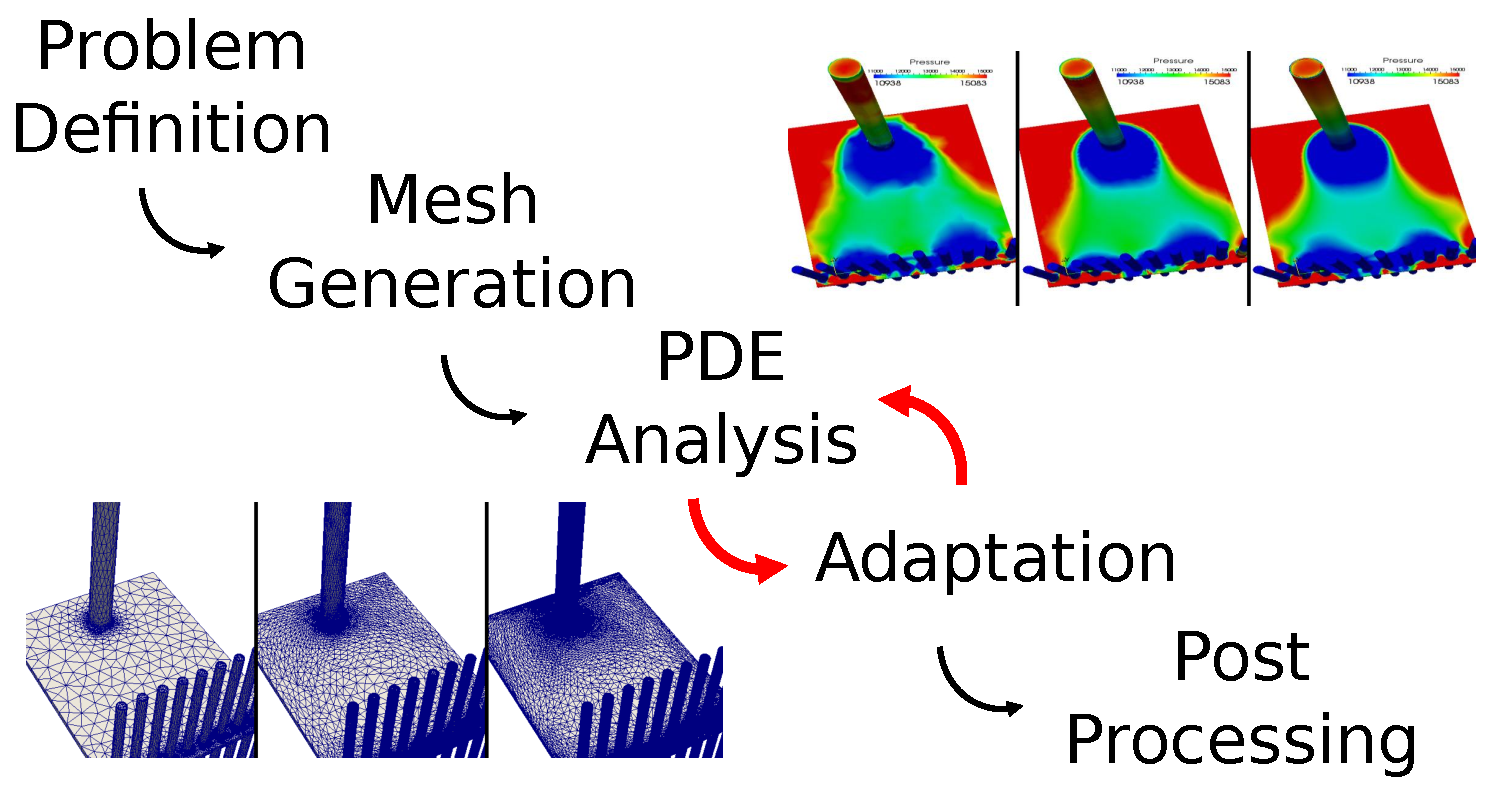
\includegraphics[width=.6\textwidth]{figs/SimulationBasedEngineeringWorkflow2.eps}\\
  }
  \smallskip
  Adaptive methods are critical to efficient parallel unstructured mesh-based analysis
  \begin{itemize}
    \item Anisotropic mesh adaptation can reduce the mesh size by over 10x
    \item Adaptive control of equation discretization and model application can
      yield further savings
  \end{itemize}
  Given the complexity, these analysis are often supported by multiple
  interacting components - workflows
  \begin{itemize}
    \item Components have specific requirements for their efficient execution
  \end{itemize}
\end{frame}

%----------- slide --------------------------------------------------%
\begin{frame}
  \frametitle{Adaptive Workflows}
  At scale performance bottlenecks exist during the data transformation
  within components and during the data transfer between components\\
  \begin{itemize}
    \item Load balancing graph and geometric based methods either consume too
      much memory and fail, or produce such low quality partitions that they are
      ineffective for analysis
    \item File-based inter-component transfers relying on the (s)lowest level of the
      memory hierarchy do not scale at the same rate as the compute nodes
  \end{itemize}
  This thesis addresses these limitations via
  \begin{itemize}
    \item Efficient multi-criteria partition improvement, and
    \item In-memory inter-component data transfer
  \end{itemize}
  And demonstrates their use in three in-memory adaptive workflows 
\end{frame}

%----------------------------------------------------------------------%
%----------- Section --------------------------------------------------%
%----------------------------------------------------------------------%
\section{Unstructured Mesh Partition Control}
\outline
\begin{frame}
  \frametitle{Unstructured Mesh Partition Control}
  Goals
  \begin{itemize}
    \item Improve application strong scaling on leadership systems
    \item Compliment existing partitioning methods
    \item Use a minimal amount of memory
    \item Execute in a fraction of the application's execution time
  \end{itemize}
  Approach
  \begin{itemize}
    \item Operate directly on unstructured mesh using diffusive method
    \item Use mesh adjacencies to support multiple criteria
    \item Improve scaling of applications by reducing peak imbalances
      \begin{itemize}
        \item Quickly select then migrate elements between neighboring parts
        \item Fix entity imbalances in order of applications defined priority
      \end{itemize}
  \end{itemize}
  \bigskip
  Applied to a computational fluid dynamics simulation running on 524,288
  processes with 1.24 billion elements these methods reduce the time of the
  dominant computational step by up to 28\% versus the best existing methods.
\end{frame}

%----------- slide --------------------------------------------------%
\begin{frame}
  \frametitle{Parallel Unstructured Mesh Infrastructure (PUMI)}
  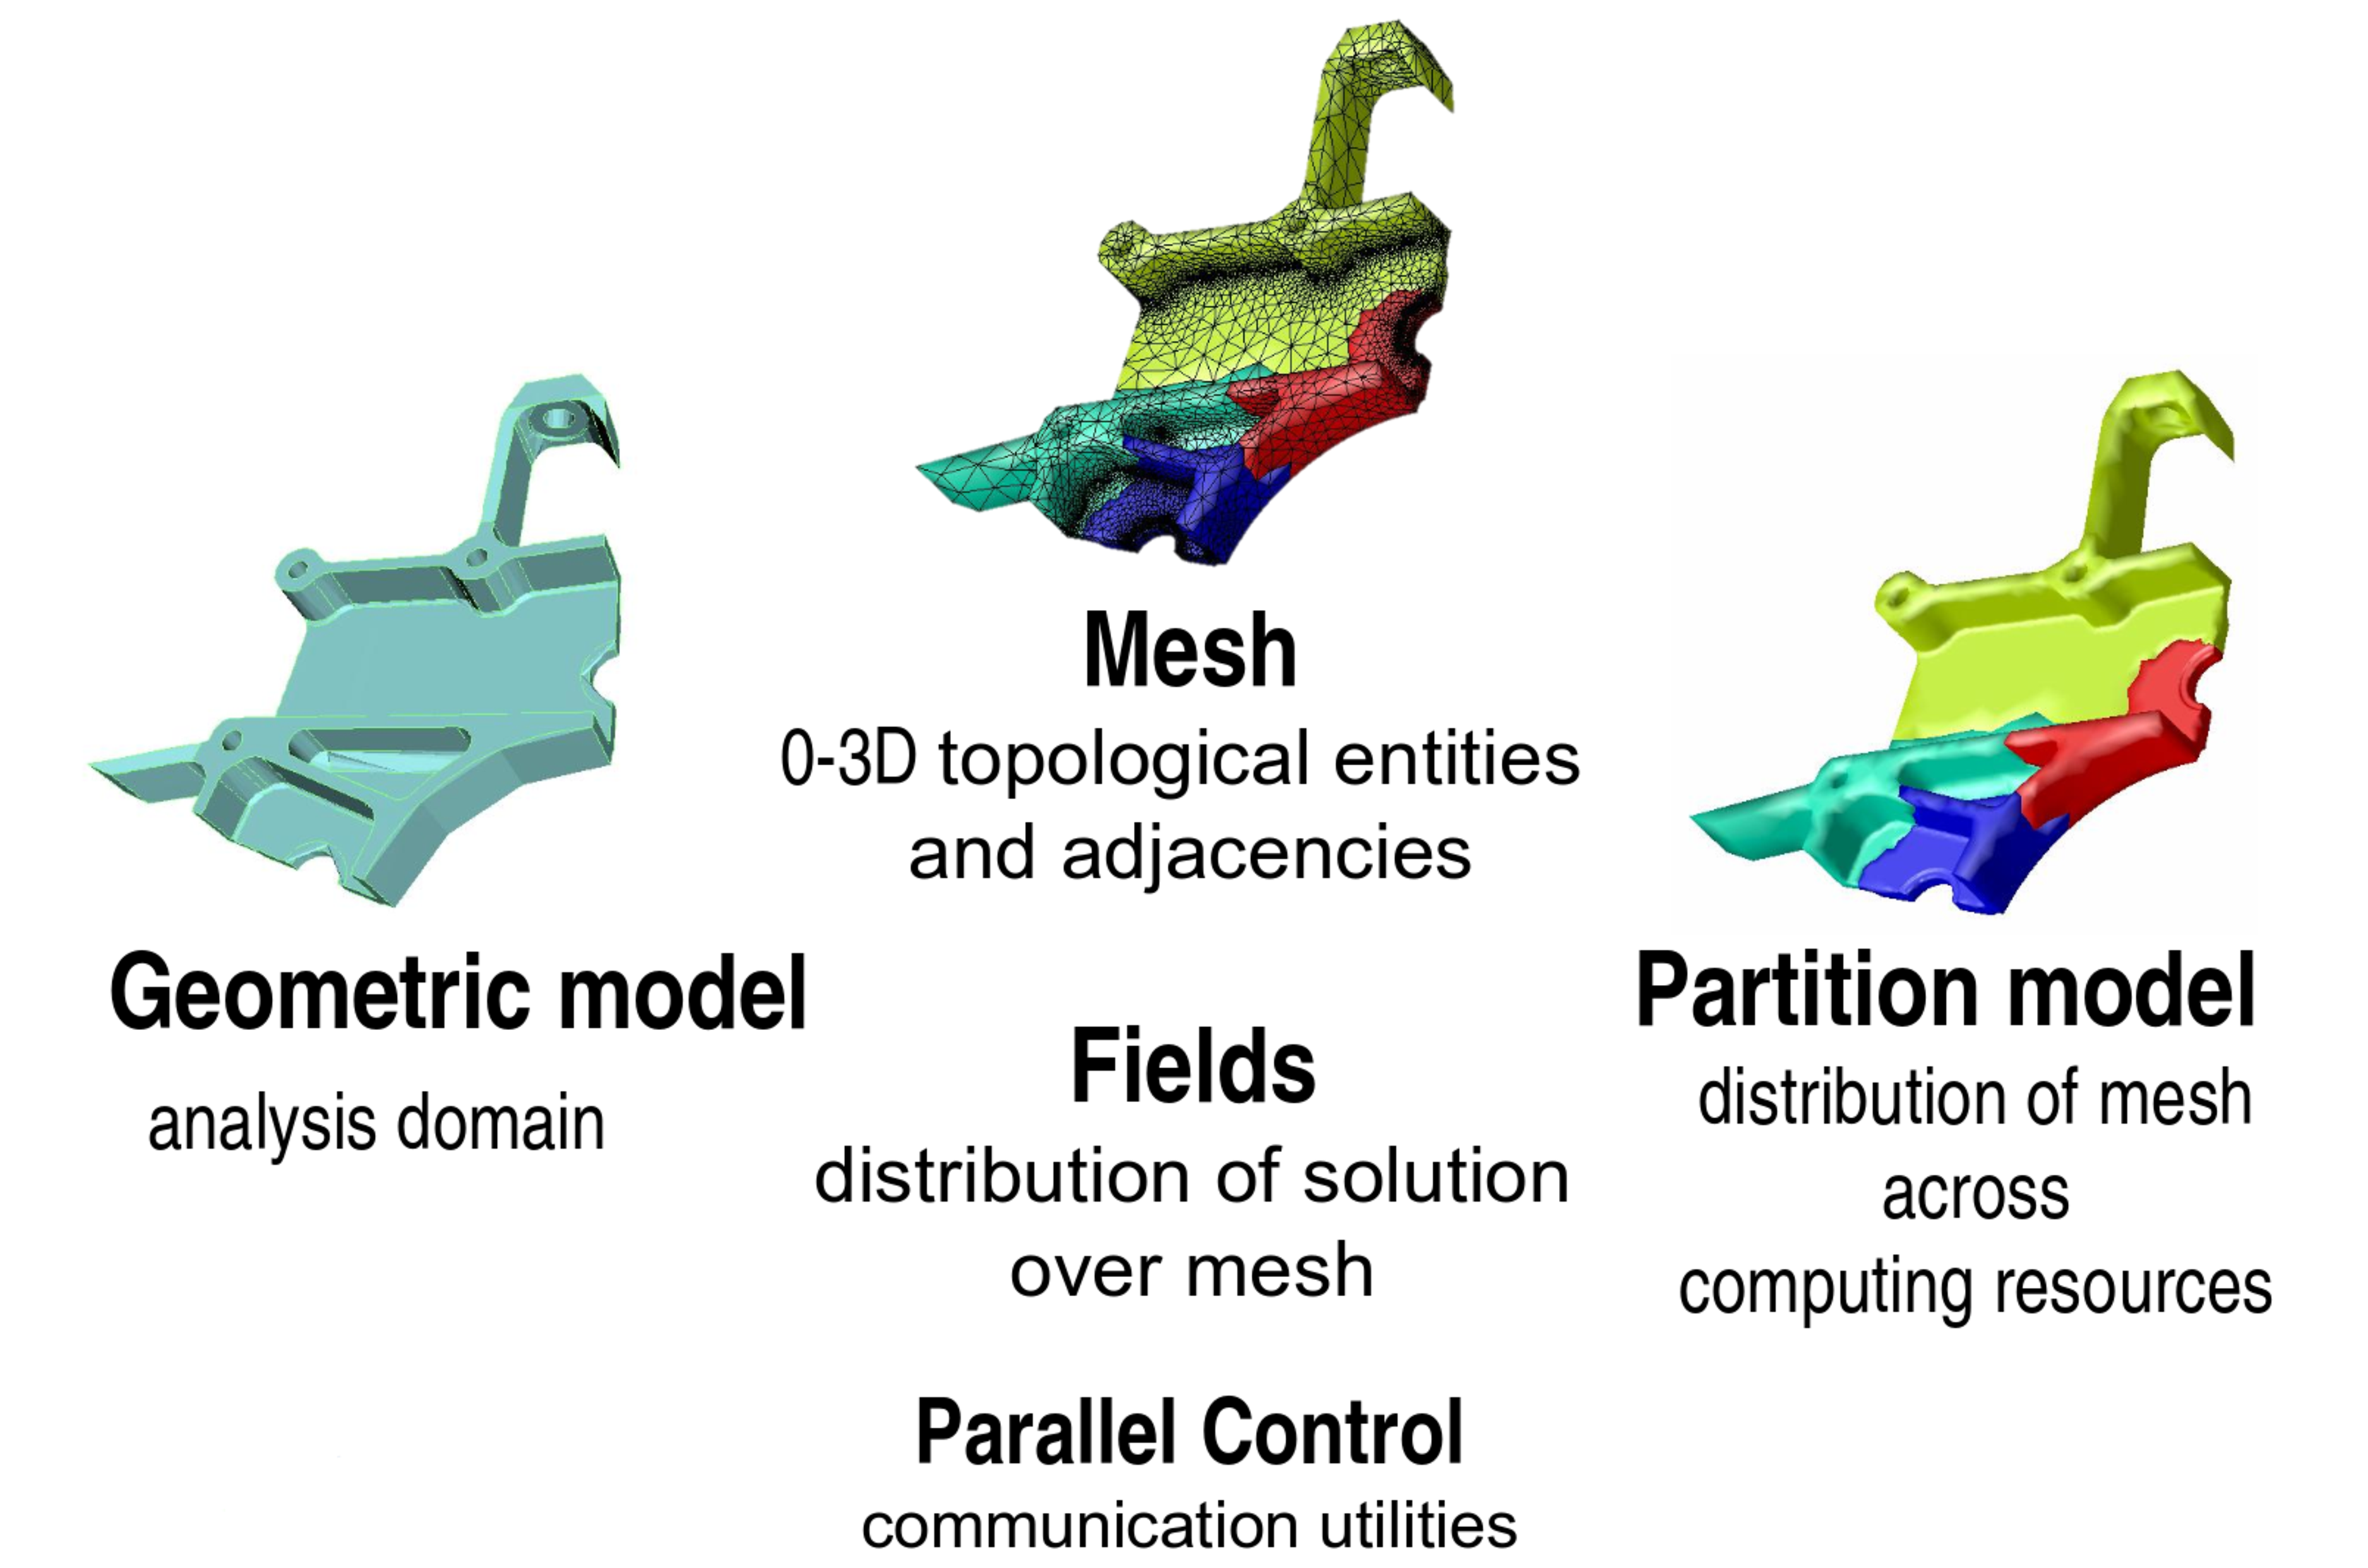
\includegraphics[width=0.95\textwidth]{figs/pumi.eps}
\end{frame}

%----------- slide --------------------------------------------------%
\begin{frame}
  \frametitle{PUMI Mesh Representation}
  Mesh entities
  \begin{itemize}
    \item vertex (0D), edge (1D), face (2D), or region (3D)
  \end{itemize}
  Adjacencies
  \begin{itemize}
    \item How the mesh entities connect to each other
    \item Complete representation: store sufficient entities and adjacencies to get any adjacency in O(1) time
  \end{itemize}
  Partition model
  \begin{itemize}
    \item Topological partition information
    \item Relationship to mesh entities – classification
  \end{itemize}
  \begin{columns}
    \begin{column}{0.1\textwidth}
      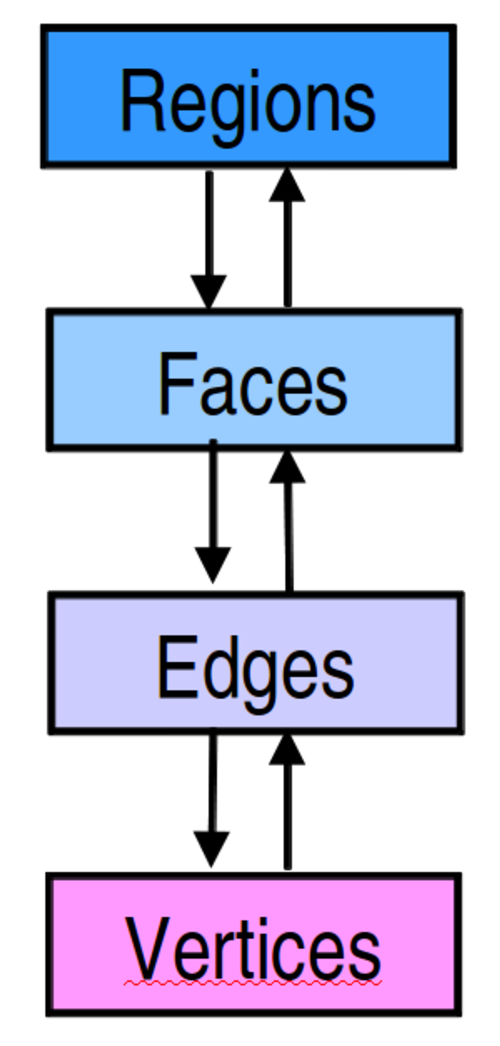
\includegraphics[width=\textwidth]{figs/meshAdj.eps}
    \end{column}
    \begin{column}{0.25\textwidth}
      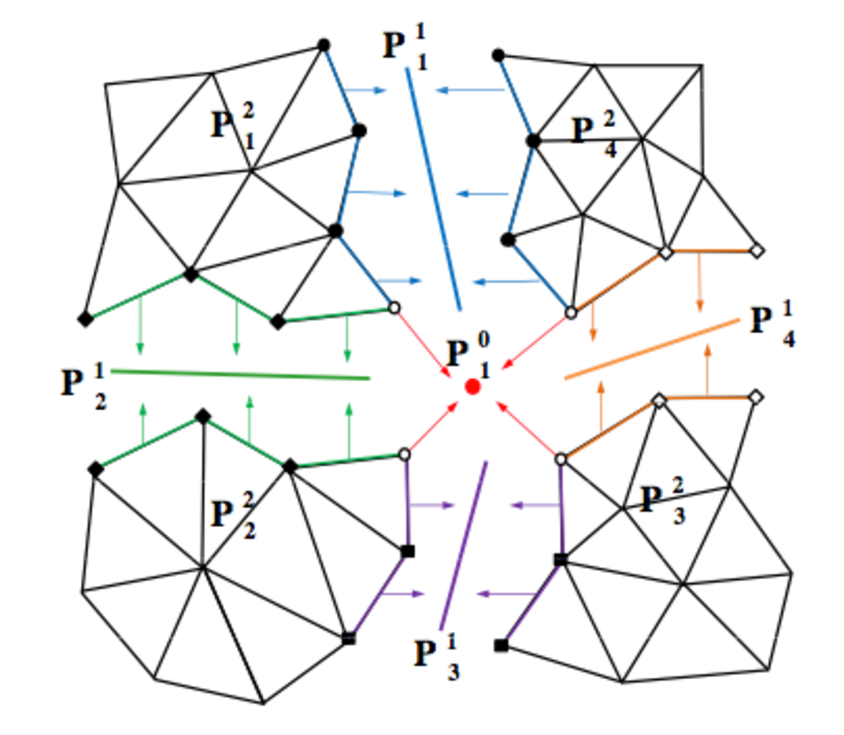
\includegraphics[width=\textwidth]{figs/sharedEnts.eps}
    \end{column}
    \begin{column}{0.25\textwidth}
      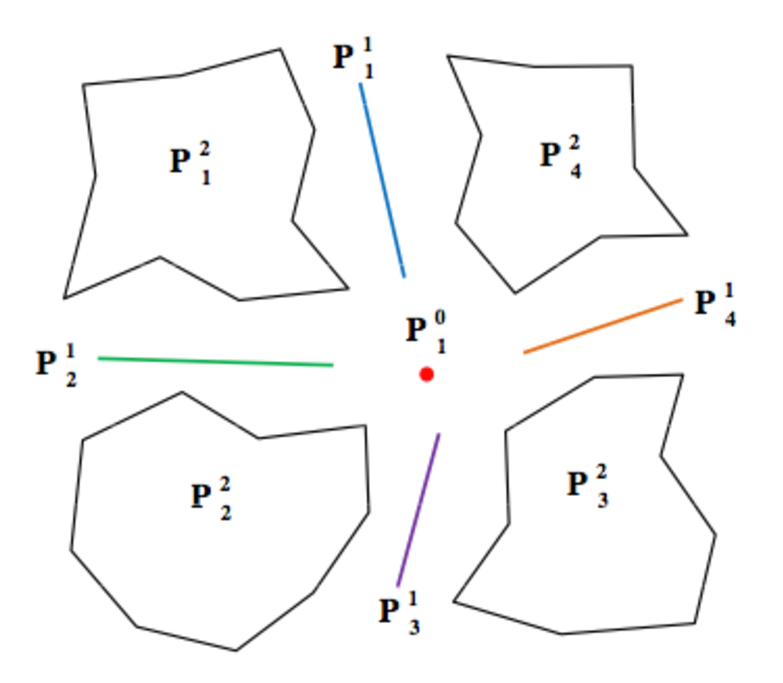
\includegraphics[width=\textwidth]{figs/partitionModelEnts.eps}
    \end{column}
    \begin{column}{0.2\textwidth}
      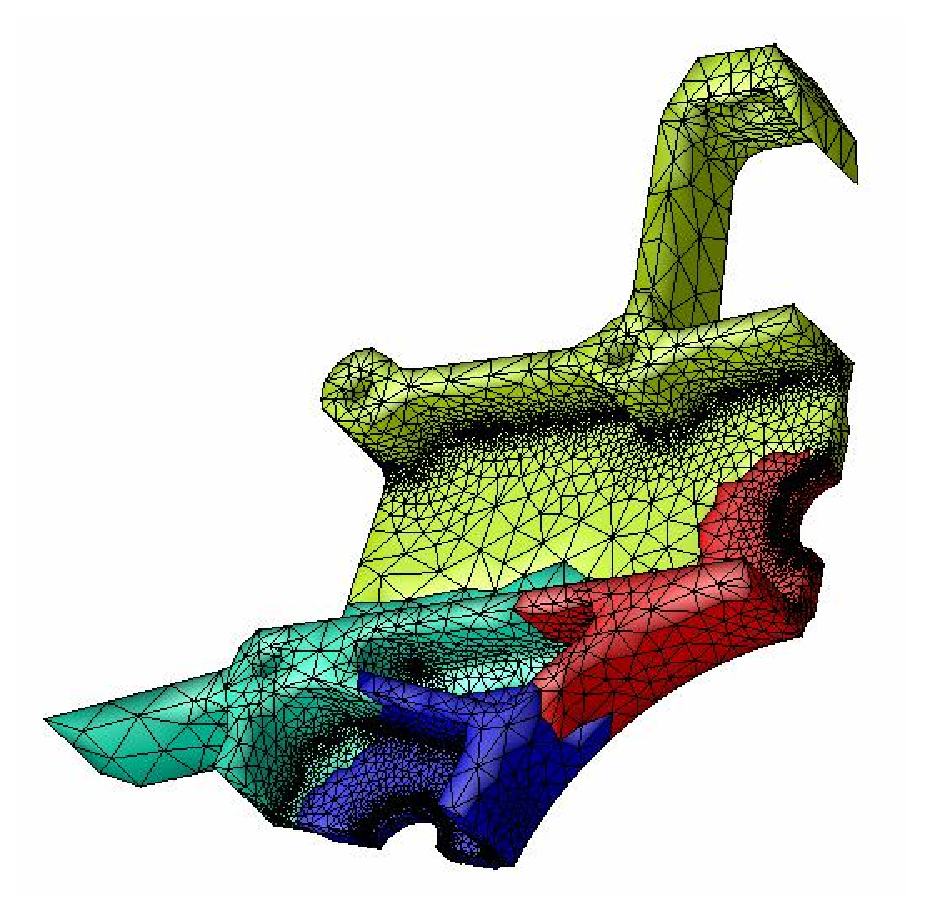
\includegraphics[width=\textwidth]{figs/partitionedMesh.eps}
    \end{column}
  \end{columns}
\end{frame}

%----------- slide --------------------------------------------------%
\begin{frame}
  \frametitle{Partitioning Methods}
  Parallel simulation requires that the mesh be distributed with equal
  work-load and minimum inter-part communications \\
  \bigskip
  Graph and hypergraph based partitioners
  \begin{itemize}
    \item Parallel construction and balancing of graph with small cuts
      takes reasonable time and has limited scalability
    \item Graph/hyper-graph partitions are powerful for unstructured
      meshes, however they use one dimension (as in 0,1,2,3) of mesh entity
      as the graph nodes, hence the balance of other mesh entities may
      not be optimal
  \end{itemize}
  % the following is a hack to avoid mis-aligned bullets when only using columns
  % for half the frame
  \vskip-10pt
  \mbox{}\hfill\raisebox{-\height}[0pt][0pt]{
    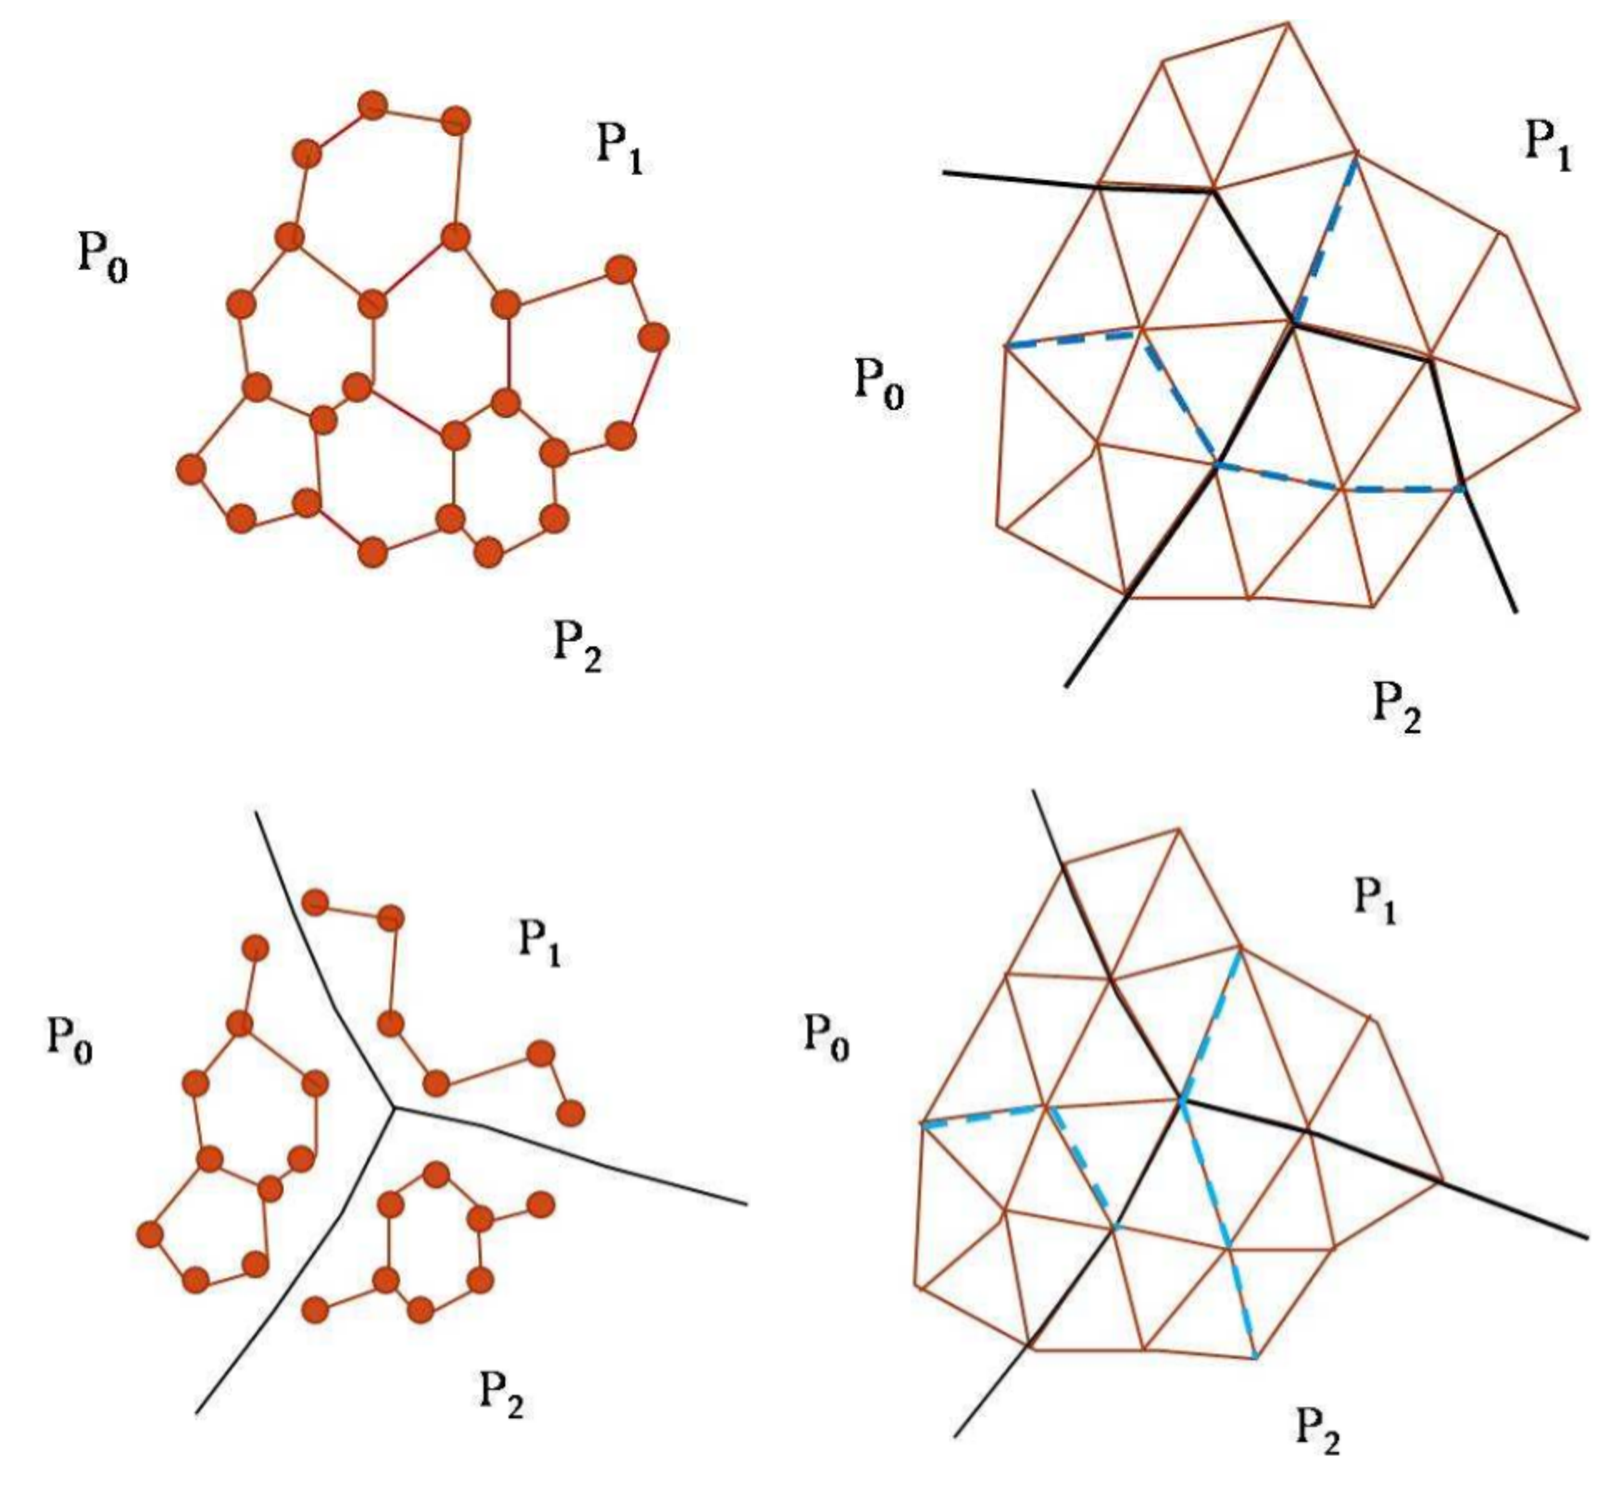
\includegraphics[width=.30\textwidth]{../parmaimprovement/figs/localVsGlobalZhou.eps}
  }\\
  Geometric partitioners
  \begin{itemize}
    \item \lenitem{Inexpensive and scalable vs (hyper)graph at cost of larger
      (jagged) cuts}
  \end{itemize}
  Diffusive partitioners
  \begin{itemize}
    \item \lenitem{Quickly reduce small imbalances}
  \end{itemize}
  Local partitioners
  \begin{itemize}
    \item \lenitem{Quickly increase part count if balanced}
  \end{itemize}
\end{frame}

%----------- slide --------------------------------------------------%
\begin{frame}
  \frametitle{Partitioning using Mesh Adjacencies (ParMA)}
  Mesh and partition model adjacencies represent application data more
  completely than standard (hyper)graph-partitioning models.\\
  \medskip
  Advantages
  \begin{itemize}
    \item Avoid graph construction (assuming you have complete representation)
    \item Directly account for multiple entity types - e.g., dof holders for the solve
      process - typically the most computationally expensive step
    \item Easy to use with diffusive procedures
  \end{itemize}
  Disadvantage
  \begin{itemize}
    \item Lack of well developed algorithms for global parallel
      partitioning operations directly from mesh adjacencies
  \end{itemize}
\end{frame}

%----------- slide --------------------------------------------------%
\begin{frame}
  \frametitle{ParMA - Observations}
  \begin{columns}
    \begin{column}{.48\textwidth}
      \begin{itemize}
        \item Imbalance is often limited to a small number of heavily loaded
          parts, referred to as spikes, which limit application scalability
        \item Parts can have any shape - cannot assume they are nice and spherical
        \item Parts often have disconnected components - pairs of elements
          that don't have a face-adjacent path between them
      \end{itemize}
    \end{column}
    \begin{column}{.5\textwidth}
      \centering
      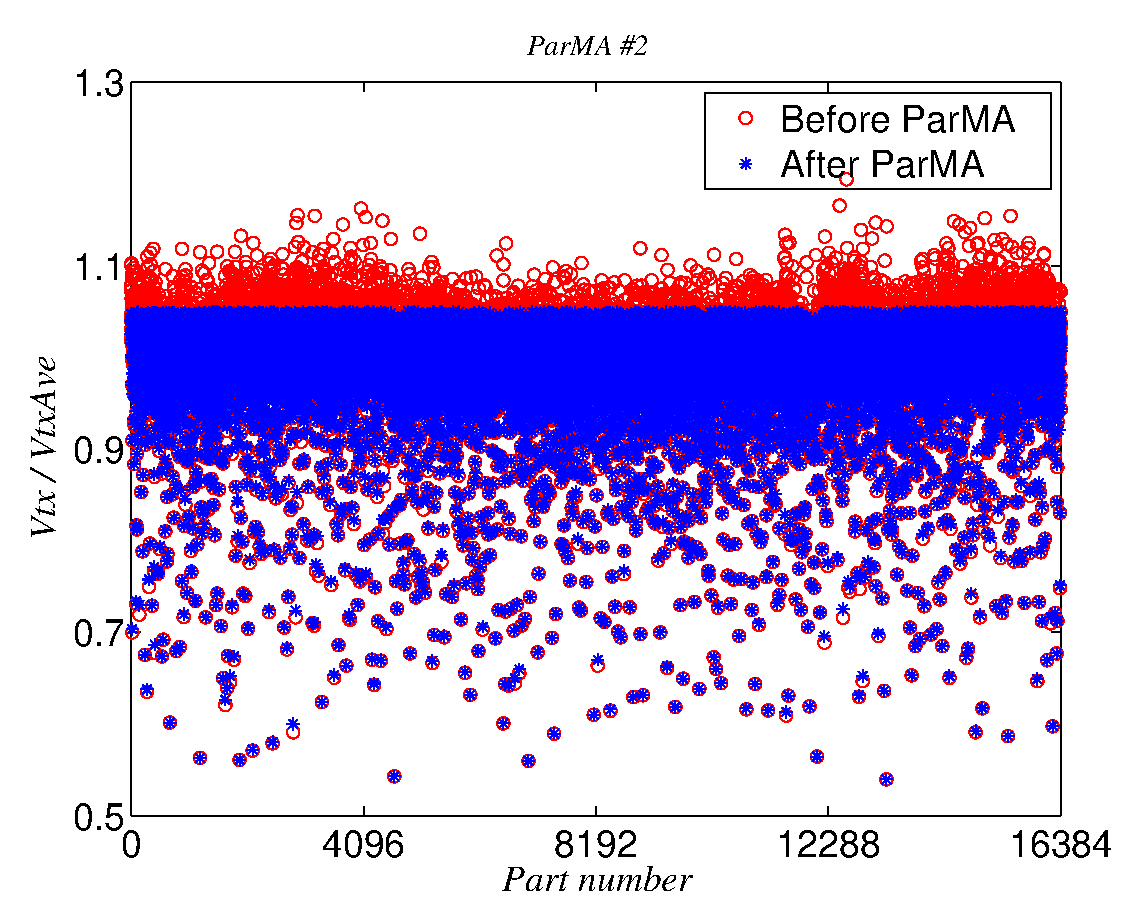
\includegraphics[width=\textwidth] {figs/numVtx16k_ver.eps}\\
      \small
      Vertex imbalance spikes.
    \end{column}
  \end{columns}
\end{frame}

%----------- slide --------------------------------------------------%
\begin{frame}
  \frametitle{ParMA - Algorithm}
  Input
  \begin{itemize}
    \item Priority list of mesh entity dimensions to be balanced (region,
      face, edge, vertex)
    \item Partitioned mesh with complete representation and entity weights
  \end{itemize}
  Algorithm
  \begin{columns}
    \begin{column}{\textwidth}
      \begin{algorithmic}
          \State list $\gets$ entity dimensions sorted by des. priority then
          asc. dimension
          \For { dimension $\in$ list  }
            \For { iter$=$0; iter $<$ maxIter; iter++ }
              \State Compute targets // Collective
              \State Select regions for migration // Embarrassingly Parallel
              \State Migrate selected regions // Collective
            \EndFor
          \EndFor
      \end{algorithmic}
    \end{column}
  \end{columns}

  \bigskip
  Ex) Rgn$>$Face$=$Edge$>$Vtx is the user's input
  \begin{itemize}
    \item improve balance for mesh regions, edges, faces, then vertices
  \end{itemize}
\end{frame}

%%----------- slide --------------------------------------------------%
\begin{frame}
  \frametitle{Targeting}
  A neighbor is a target for migration if:
  \begin{itemize}
    \item The local weight of the given entity is greater than the neighbors \emph{and}
    \item The neighbor has fewer boundary vertices than the average part \emph{and}
    \item The neighbor is lightly loaded for higher priority entity dimensions
  \end{itemize}
\end{frame}

%%----------- slide --------------------------------------------------%
\begin{frame}
  \frametitle{Selection}
  \begin{columns} 
    \begin{column}{0.5\textwidth}
       Two guiding metrics 
       \begin{itemize}
         \item Part level - order of boundary traversal
         \item Entity level - element selection
       \end{itemize}
    \end{column}
    \begin{column}{0.5\textwidth}
      \centering
      \includemedia[
        activate=pageopen,
        addresource=animations/upright_p0.mov,
        flashvars={%
          src=animations/upright_p0.mov
          &autoPlay=true
          &loop=true
          &scaleMode=stretch
        }
      ]{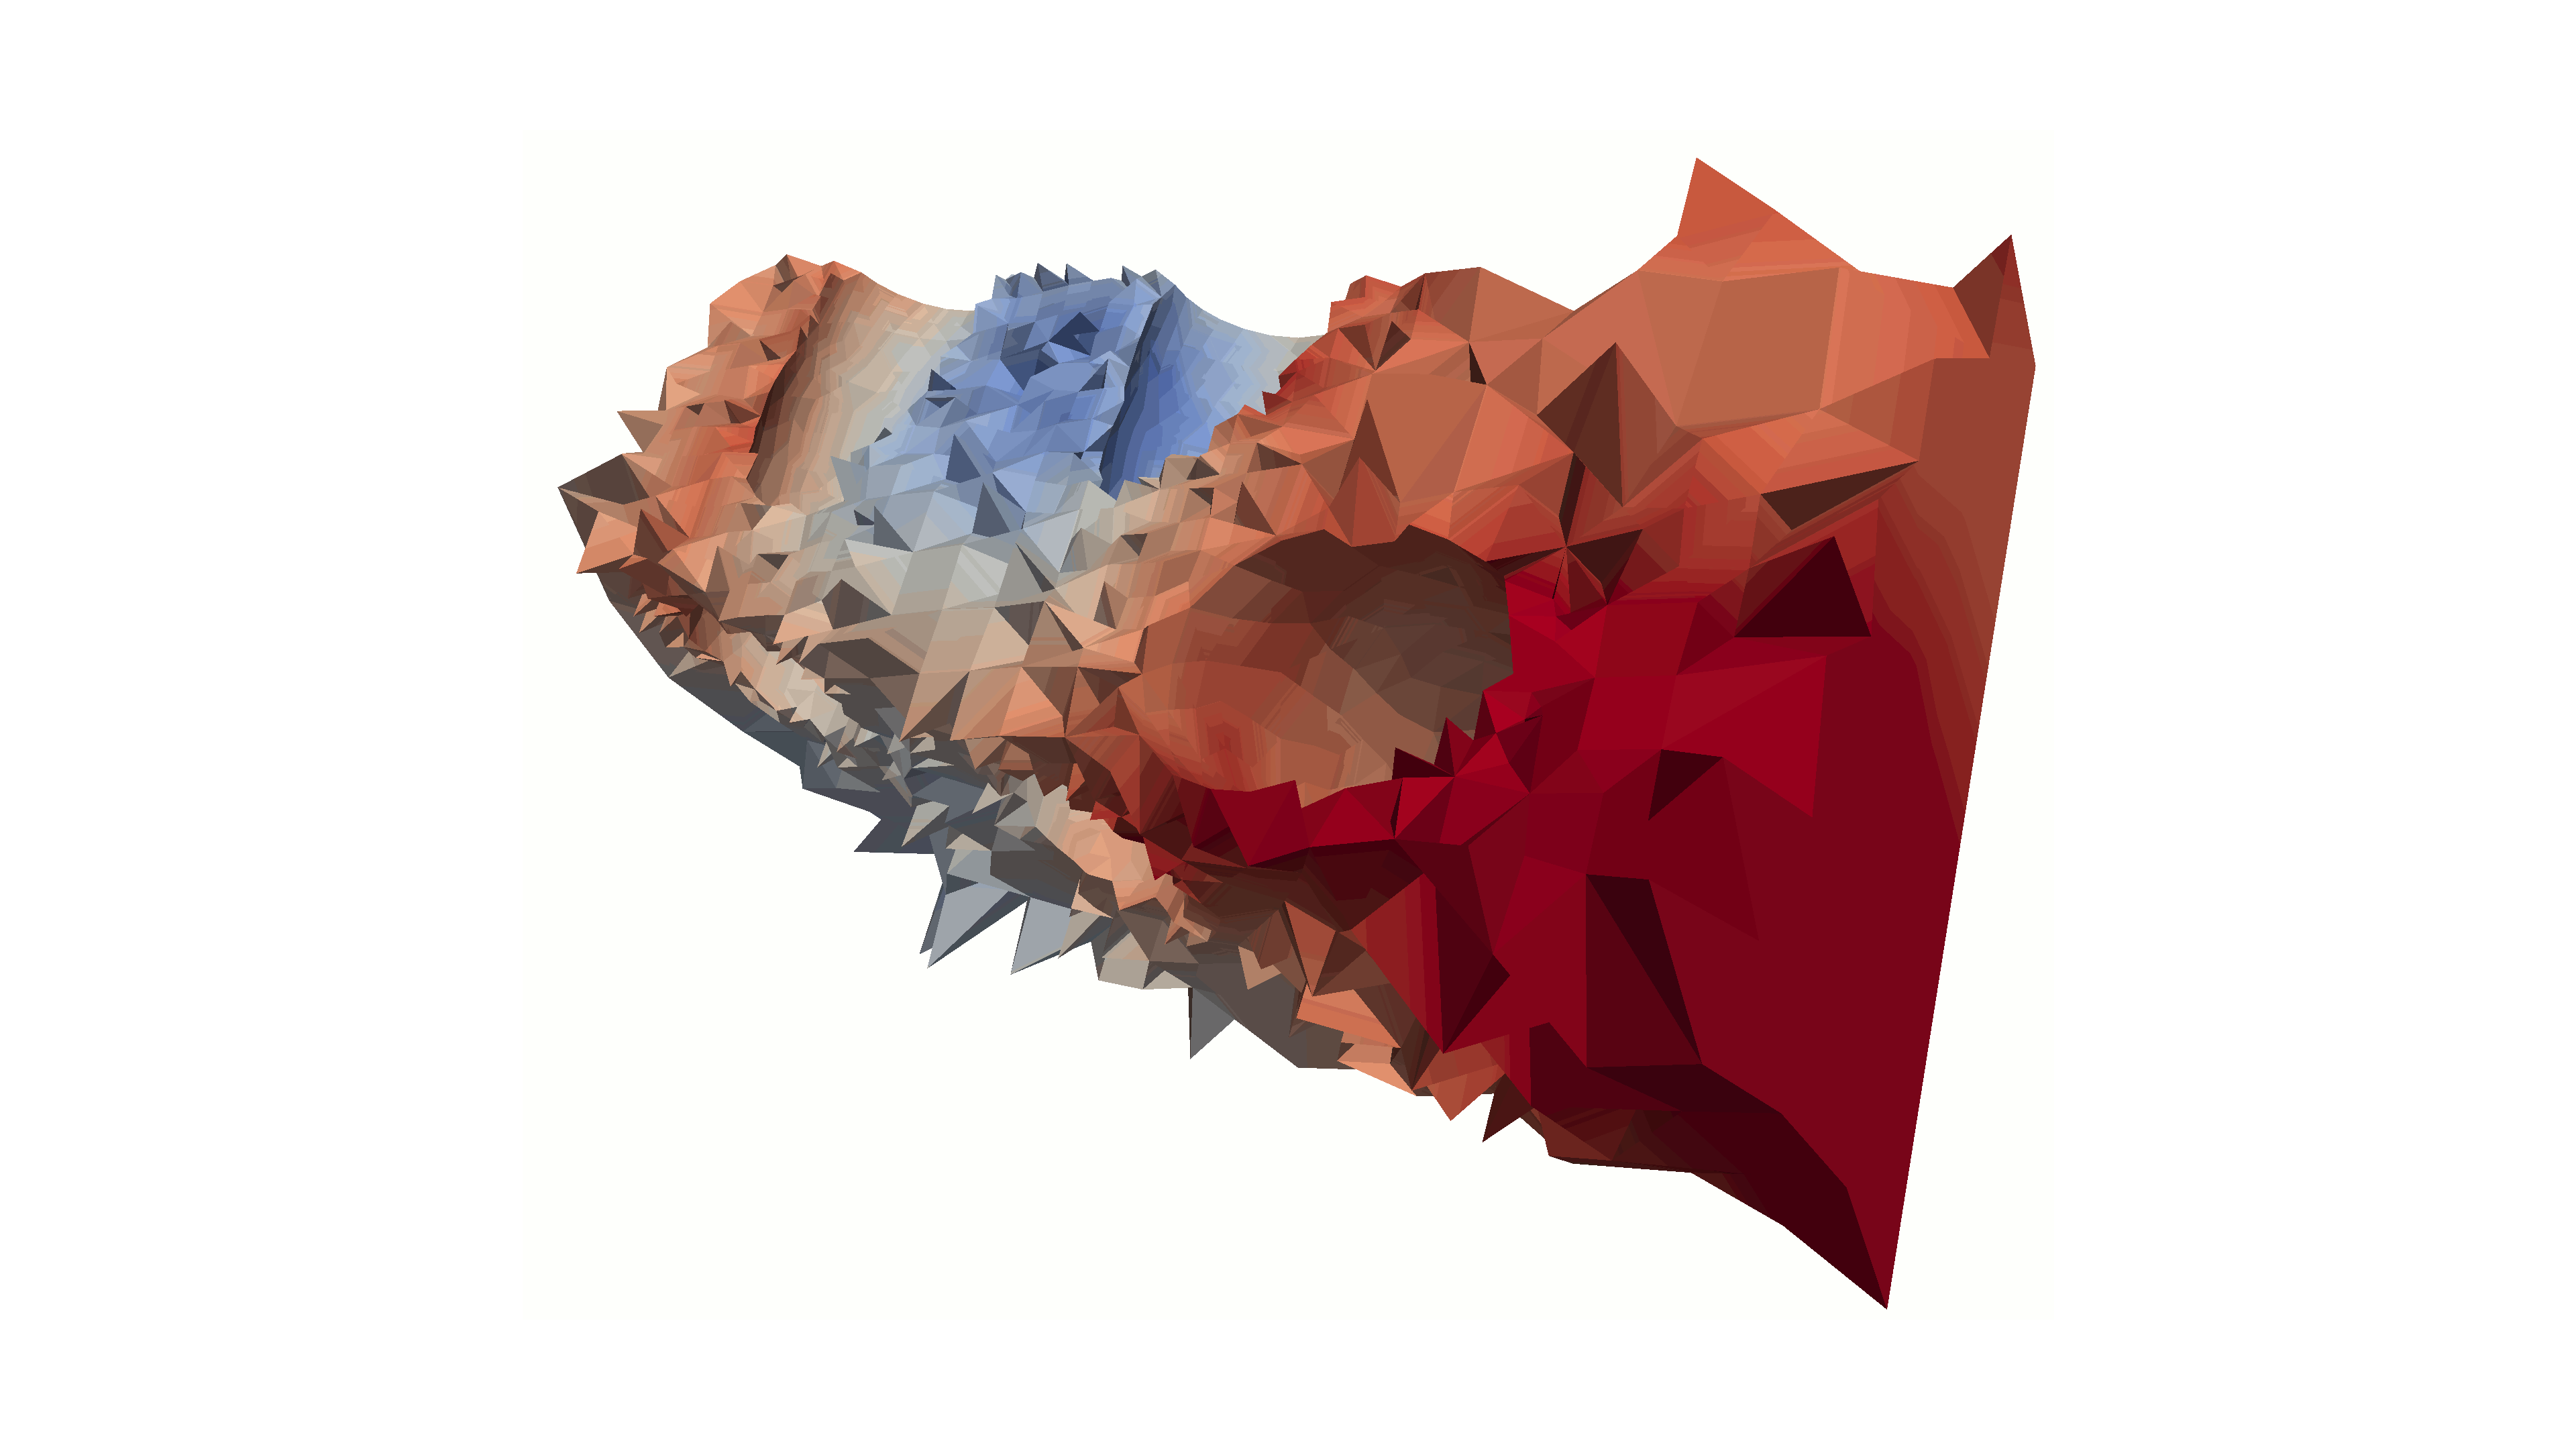
\includegraphics[width=.8\textwidth]{animations/upright_p0.png}}{StrobeMediaPlayback.swf}\\
      %{\tiny Vist vertices in order of topological distance (red to blue).}
    \end{column}
  \end{columns}
  \vskip-10pt
  \mbox{}\hfill\raisebox{-4\height}[0pt][0pt]{
    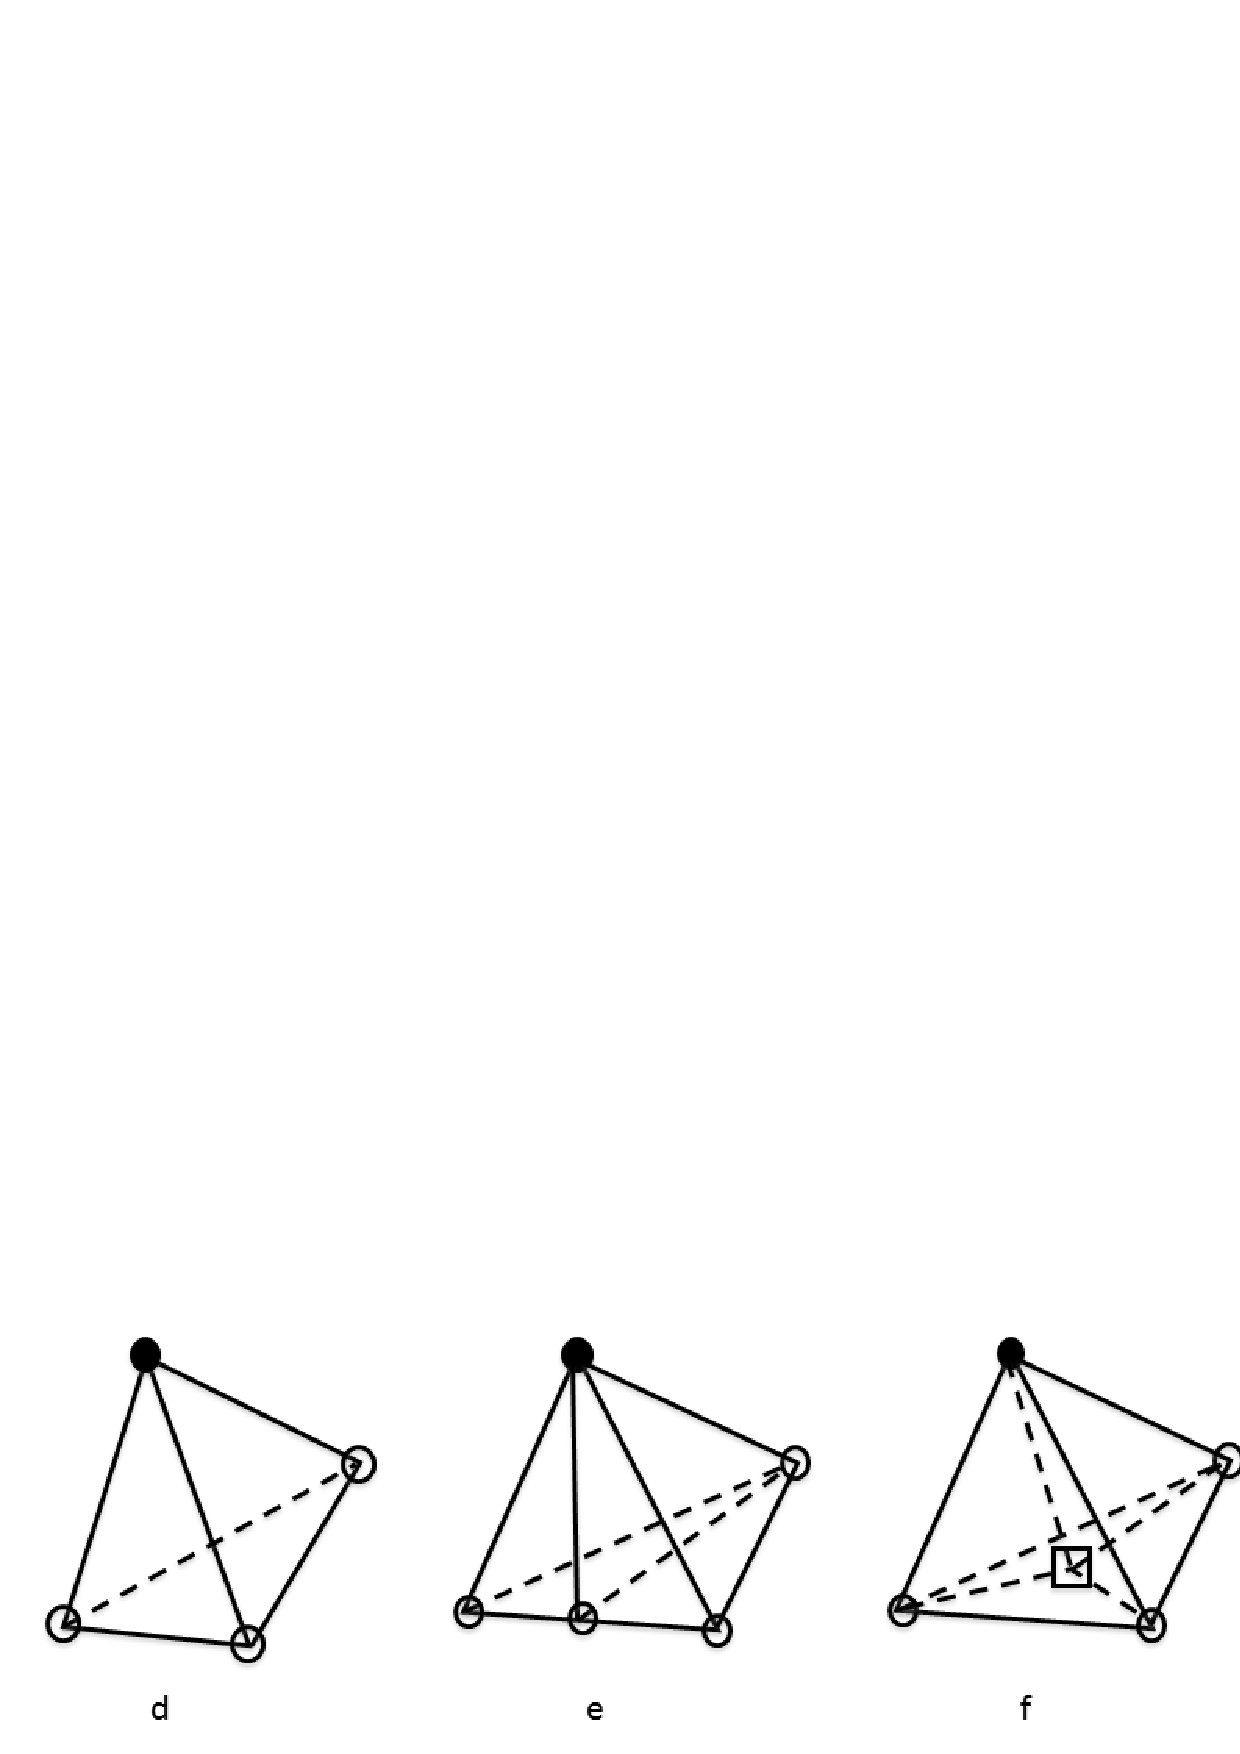
\includegraphics[width=.3\textwidth]{{figs/vertexCavities.png}.eps}
  }\\
  Part level - Component Graph Distance
  \begin{itemize}
    \item Breadth-first traversal from part boundary to locate
      deepest level
    \item One vertex from each edge connected set of deepest vertices
      is the components core
    \item Dijkstra's shortest path to compute graph distance from 
      core to the other component vertices
  \end{itemize}
  Entity level - Cavity size, topology, and connections
  \begin{itemize}
    \item Traverse boundary vtx by descending distance
    \item Construct cavity of unmarked bounded elms
    \item Find neighbor with highest surface area
    \item Select cavity if it's `small' and under transfer limit
    \item Repeat with increasing cavity size limit
  \end{itemize}
  % the following is a hack to avoid mis-aligned bullets when only using columns
  % for half the frame
\end{frame}

%----------------------------------------------------------------------%
%----------- SubSection -----------------------------------------------%
%----------------------------------------------------------------------%
\subsection{ParMA Results}

%----------- slide --------------------------------------------------%
\begin{frame}
  \frametitle{LIIPBMod Comparison}
  \begin{columns} 
    \begin{column}{0.5\textwidth}
      Test setup
      \begin{itemize}
        \item ParMA vtx$>$elm improvement versus LIIPBMod vtx improvement
        \item 64Ki, 128Ki, and 256Ki partition of a 941 million element
          AAA tet mesh
        \item Mesh generated by successively refining an initial coarse mesh
        \item Partitions created by running local ParMETIS on a 16Ki base
          partition created with global ParMETIS.
        \item Ran on the Mira Blue Gene/Q system using one part per hardware
          thread
      \end{itemize}
    \end{column}
    \begin{column}{0.5\textwidth}
      \centering
      \includegraphics[width=\textwidth]{../parmaimprovement/results/liipbmod-v-parma/aaa-a1m2/modelAnd1pt8MelmMesh.eps}\\
      \small
      Abdominal aortic aneurysm (AAA) geometric model and close-up view of a
      coarse mesh.
    \end{column}
  \end{columns}
\end{frame}

%----------- slide --------------------------------------------------%
\begin{frame}
  \frametitle{LIIPBMod Comparison}
  \begin{columns} 
    \begin{column}{0.5\textwidth}
      Results
      \begin{itemize}
        \item LIIPBMod targets a 5\% vtx imb. but stagnates at 10\%
        \item ParMA targets and achieves a 5\% vertex and element imbalance
        \item ParMA executes 75\% faster than LIIPBMod
        \item ParMA \& LIIPBMod have an insignificant ($<$1\%) effect on the total
          number of vertices
      \end{itemize}
    \end{column}
    \begin{column}{0.5\textwidth}
      \centering
      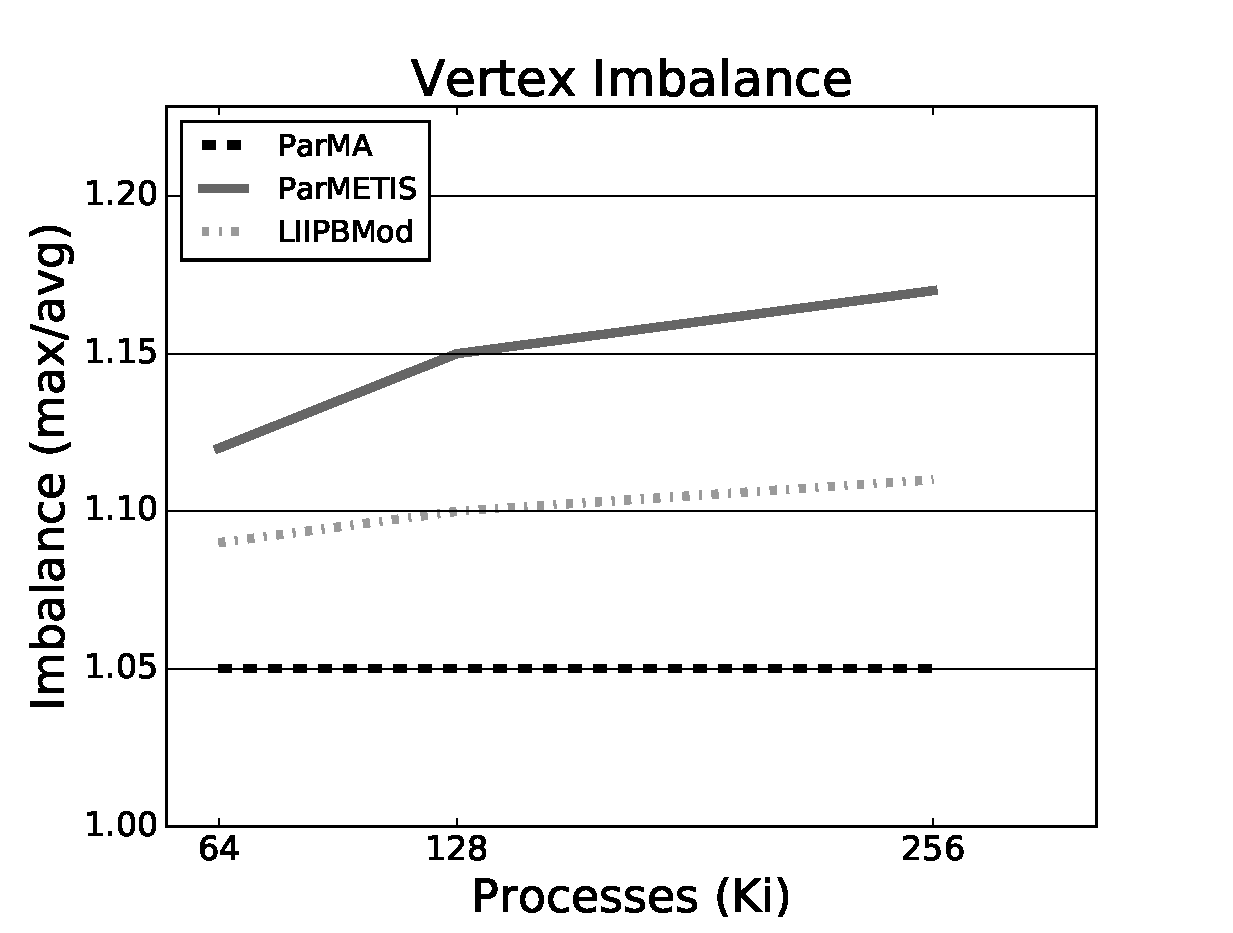
\includegraphics[width=.8\textwidth]{../parmaimprovement/results/liipbmod-v-parma/vtxImb.eps}\\
      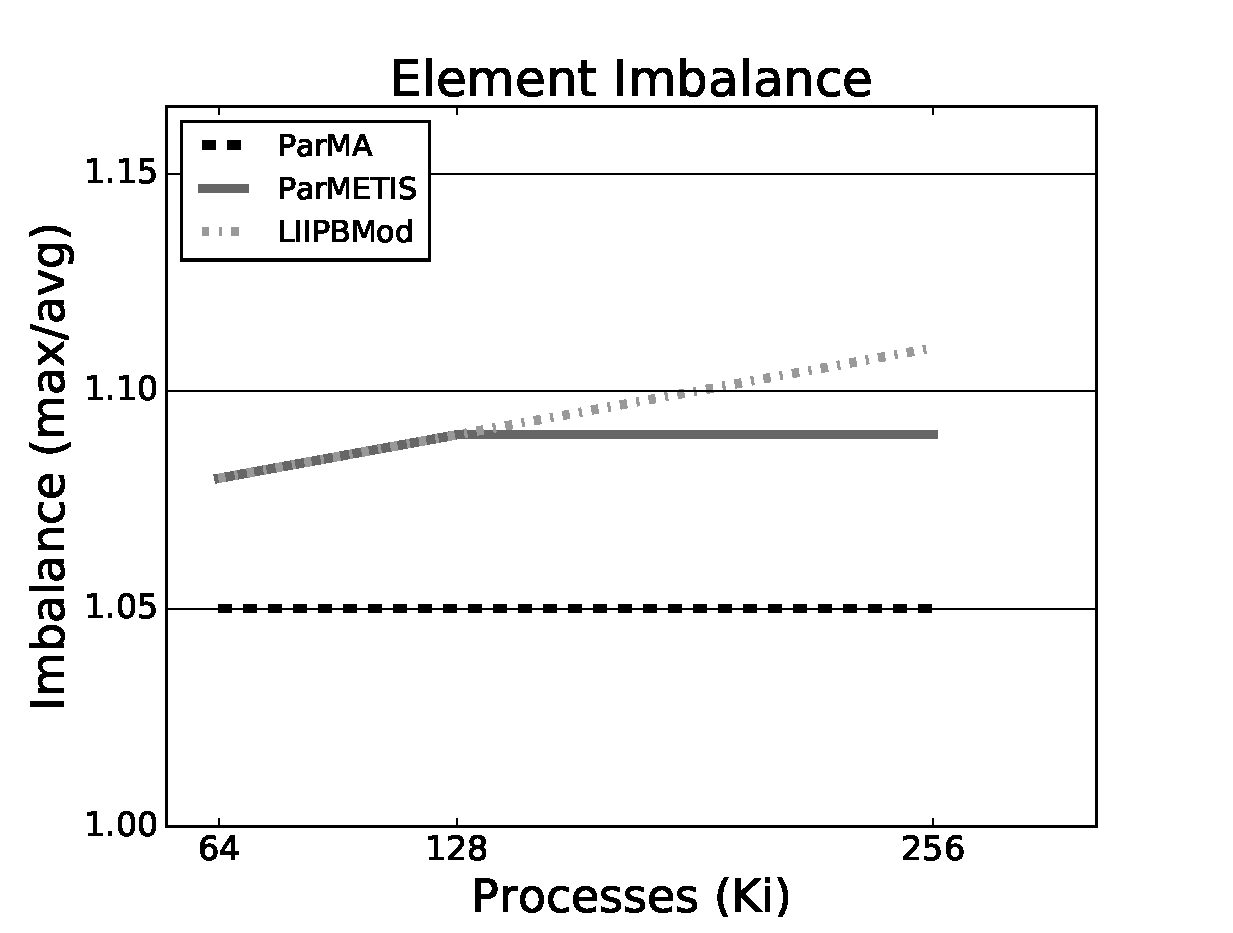
\includegraphics[width=.8\textwidth]{../parmaimprovement/results/liipbmod-v-parma/elmImb.eps}\\
      \small
      ParMA, LIIPBMod, and ParMETIS vtx (top) and elm (bottom) imbalance.
    \end{column}
  \end{columns}
\end{frame}

%----------- slide --------------------------------------------------%
\begin{frame}
  \frametitle{Partitioning to 1,048,576 Parts}
  Multiple tools needed to maintain partition quality at scale
  \begin{itemize}
    \item Local and global topological and geometric methods
    \item ParMA quickly reduces large imbalances and improves part shape
  \end{itemize}
  Partitioning 1.6B element mesh from 128K to 1Mi parts (1.5k elms/part)
  then running ParMA.  128K partition has less than 7\% imbalance.
  \setbeamerfont{itemize/enumerate body} {size=\small}
  \begin{itemize}
    \item Global RIB - 103 seconds, ParMA - 20 seconds results in:\\
      209\% vtx imb reduced to 6\%, perfect elm imb increased to 4\%, and
      5.5\% reduction in avg vtx per part
    \item Local ParMETIS - 9.0 seconds, ParMA - 9.4 seconds results in:\\
      63\% vtx imb reduced to 5\%, 12\% elm imb reduced to 4\%, and
      2\% reduction in avg vtx per part
  \end{itemize}
  Partitioning 12.9B element mesh from 128K ($<$ 7\% imb) to 1Mi parts (12k
  elms/part) then running ParMA.
  \begin{itemize}
    \item Local ParMETIS - 60 seconds, ParMA - 36 seconds results in:\\
      35\% vtx imb to 5\%, 11\% elm imb to 5\%, and
      0.6\% reduction in avg vtx per part
  \end{itemize}
  \small
  Ran on ALCF's Mira Blue Gene/Q with one hardware thread per part\\
\end{frame}

%----------- slide --------------------------------------------------%
\begin{frame}
  \frametitle{PHASTA Performance Improvement}
  \begin{itemize}
    \item 1.2B element anisotropic mesh generated via error-field based
      adaptation on 4Ki parts $\rightarrow$ global ParMETIS to 8Ki
    \item Local ParMETIS applied to 8Ki partition to create 64Ki, 128Ki,
      256Ki, and 512Ki partitions 
    \item ParMA ran on each partition with one core per part \\
     - up to 512Ki cores on 32 racks of Blue Gene/Q
 \end{itemize}
  \begin{columns} [t]
    \begin{column}{0.45\textwidth}
      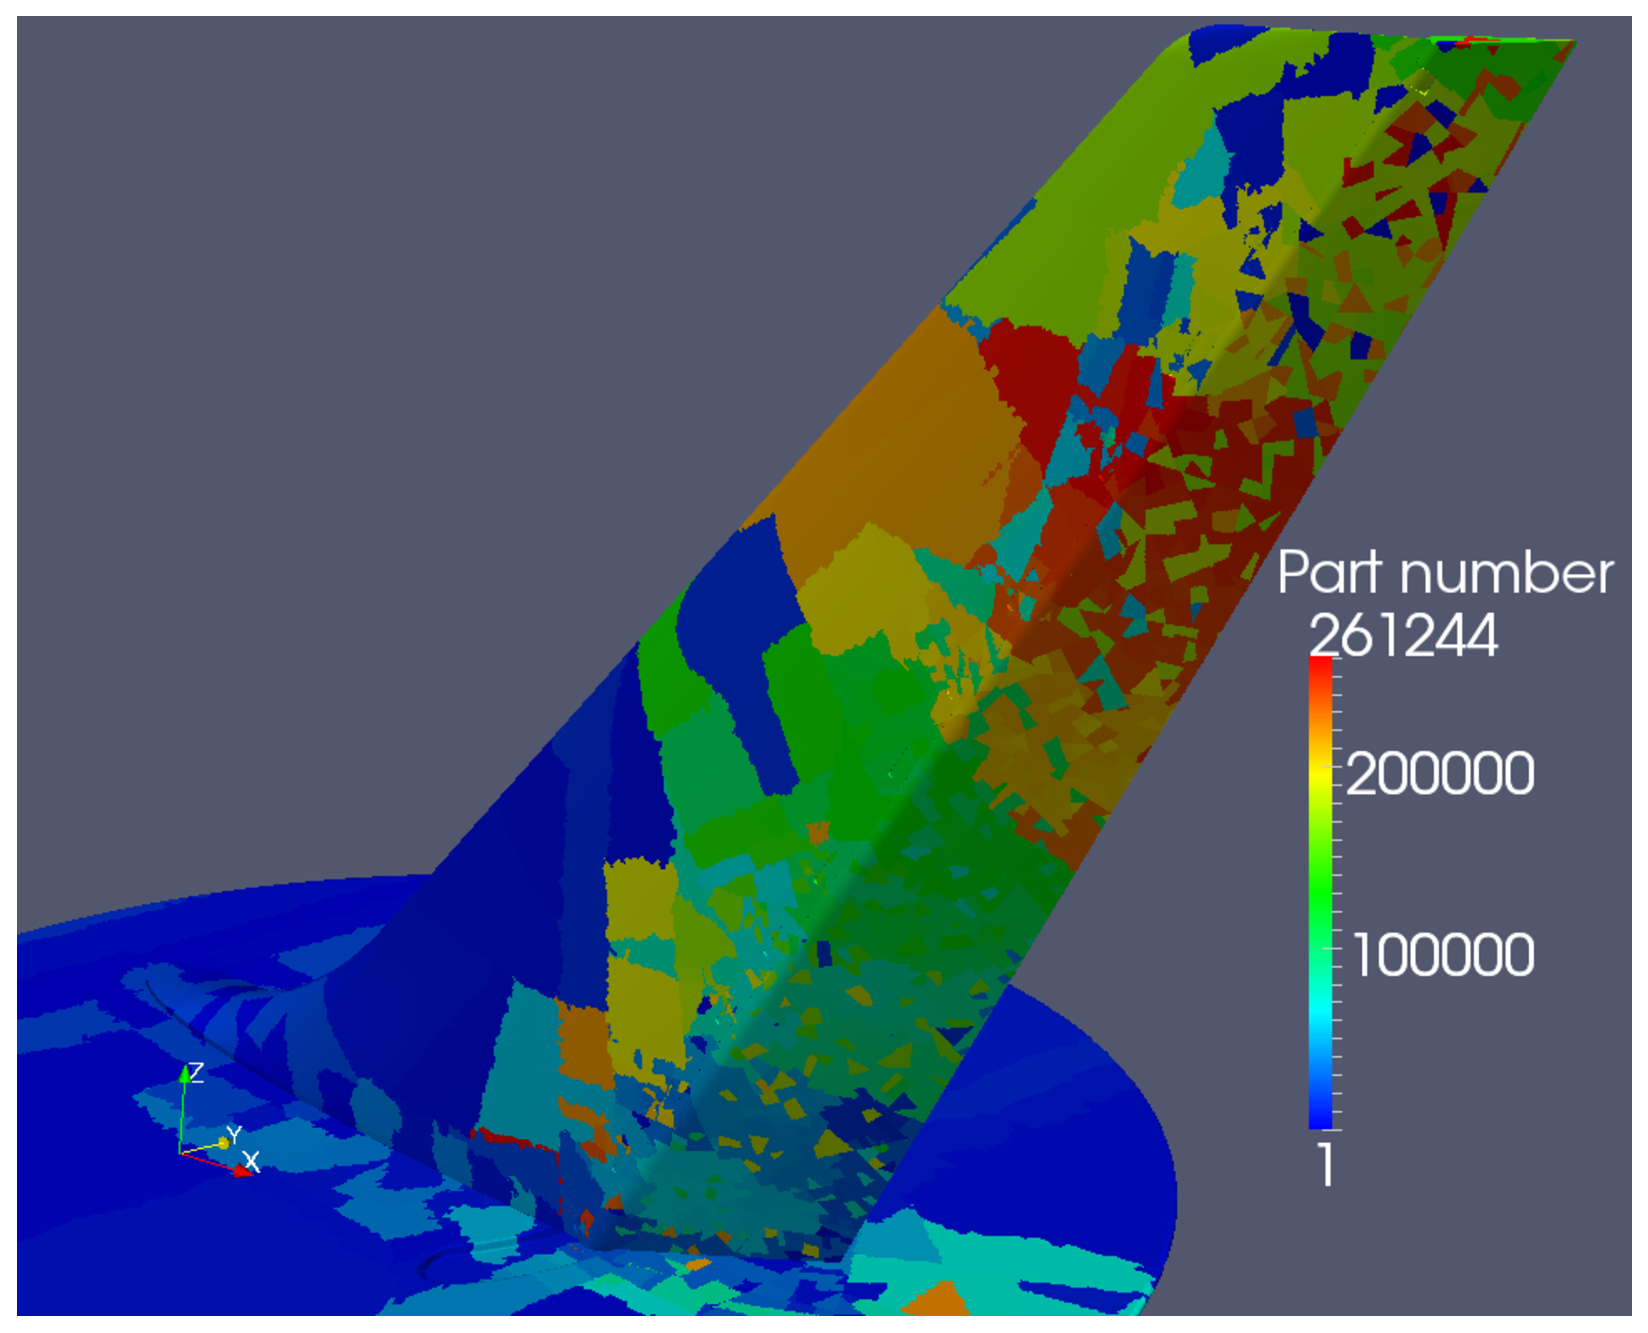
\includegraphics[width=\textwidth]{../parmaimprovement/results/phasta/stabilizerFullView.eps}
    \end{column}
    \begin{column}{0.45\textwidth}
      \centering
      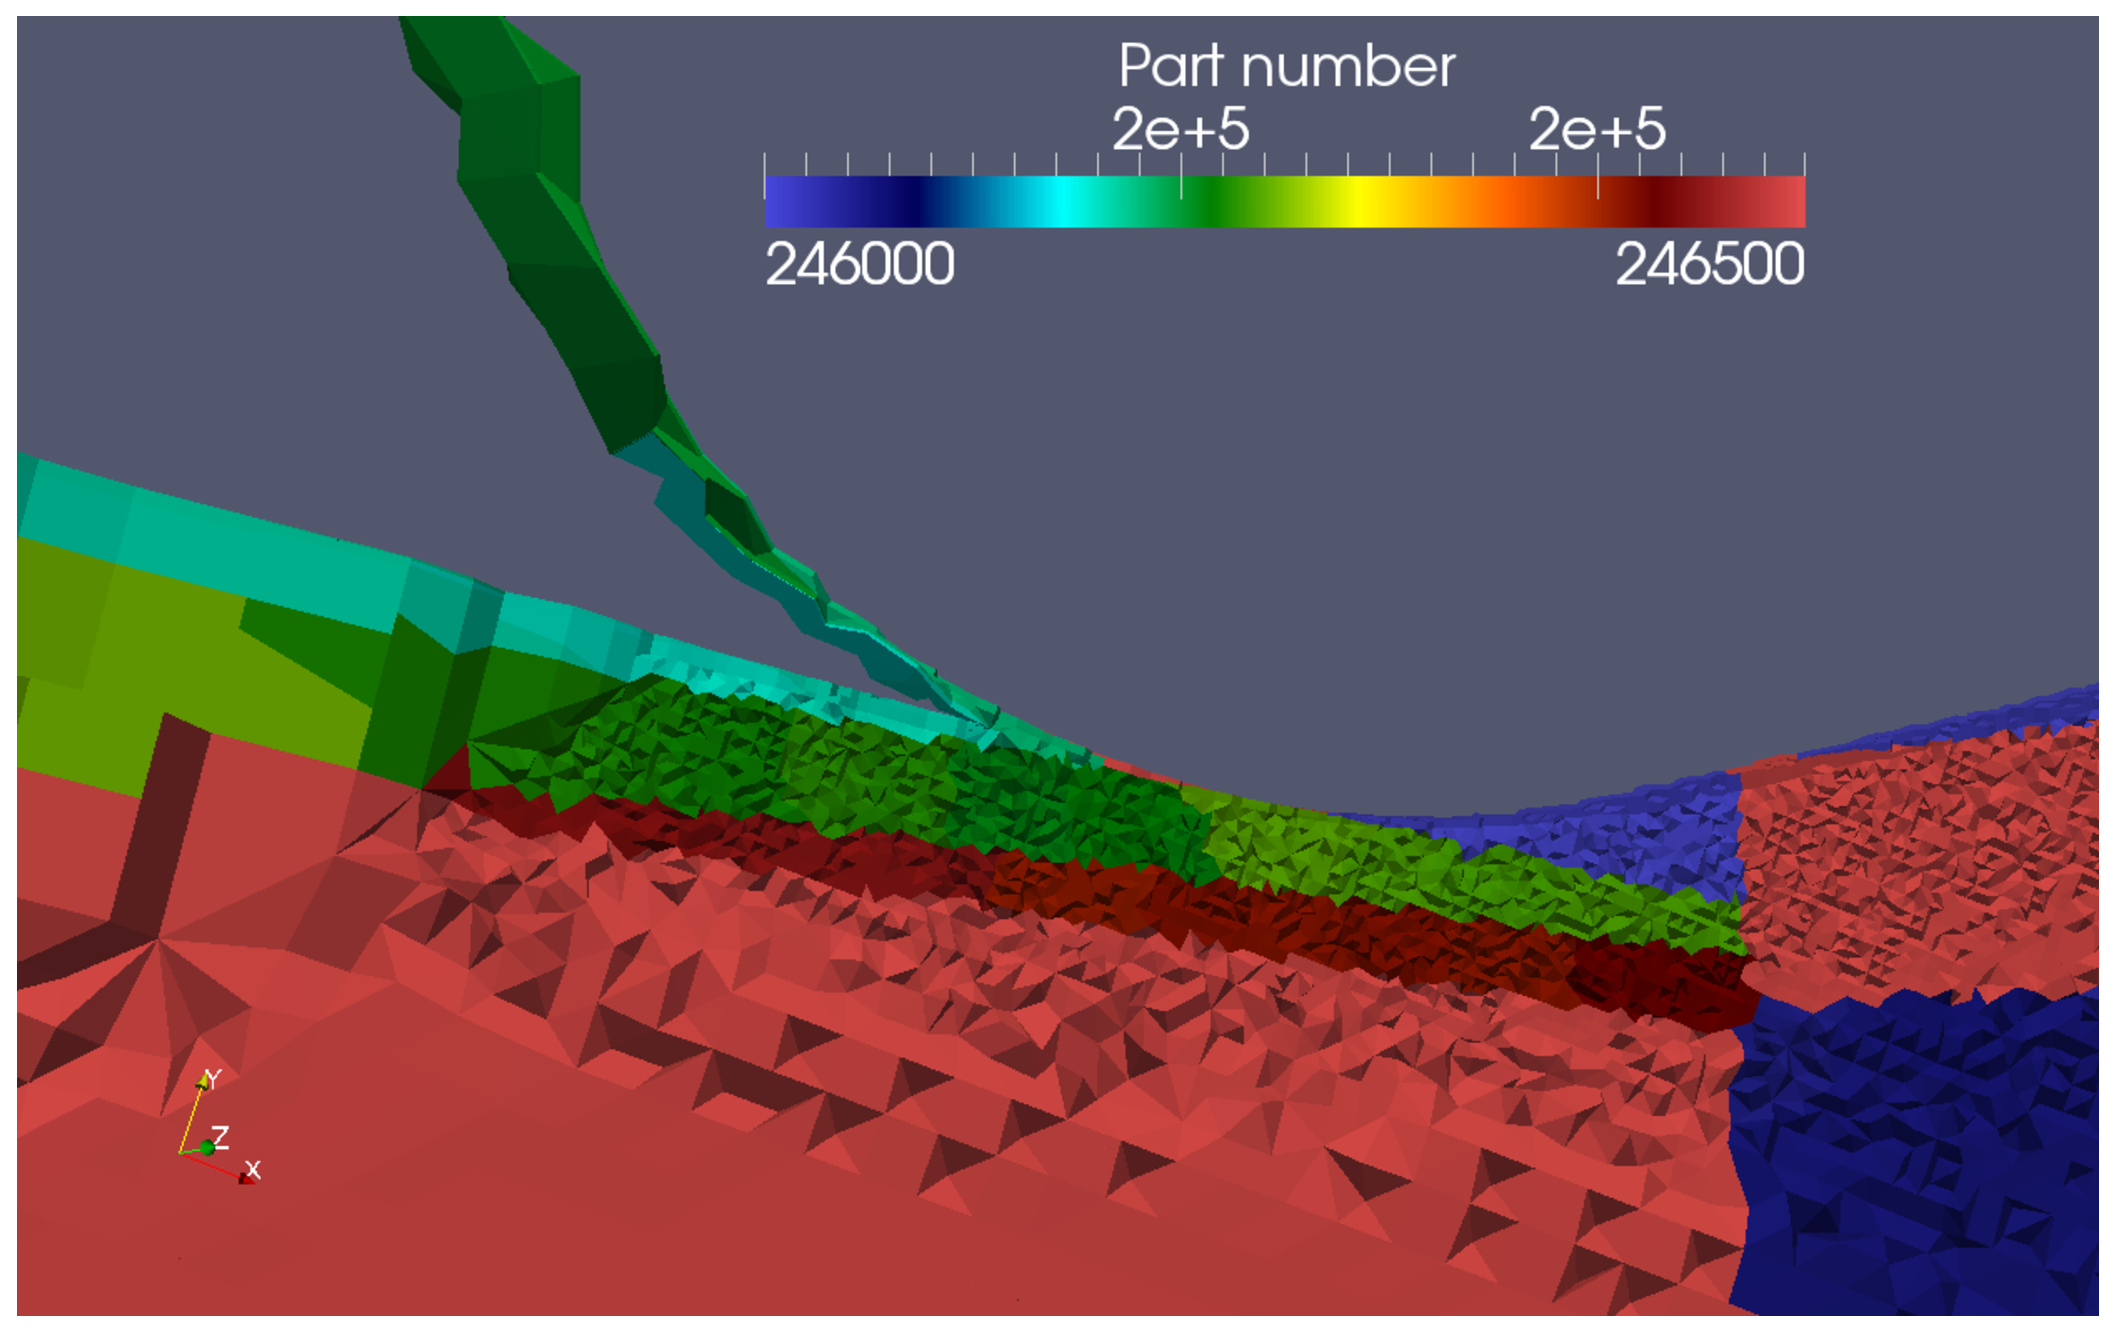
\includegraphics[width=\textwidth]{../parmaimprovement/results/phasta/stabilizerGap.eps}
    \end{column}
  \end{columns}
  \small
  (left) vertical stabilizer and rudder and (right) a slice at their junction
\end{frame}

%----------- slide --------------------------------------------------%
\begin{frame}
  \frametitle{PHASTA Performance Improvement - Entity Imbalance}
  \centering
  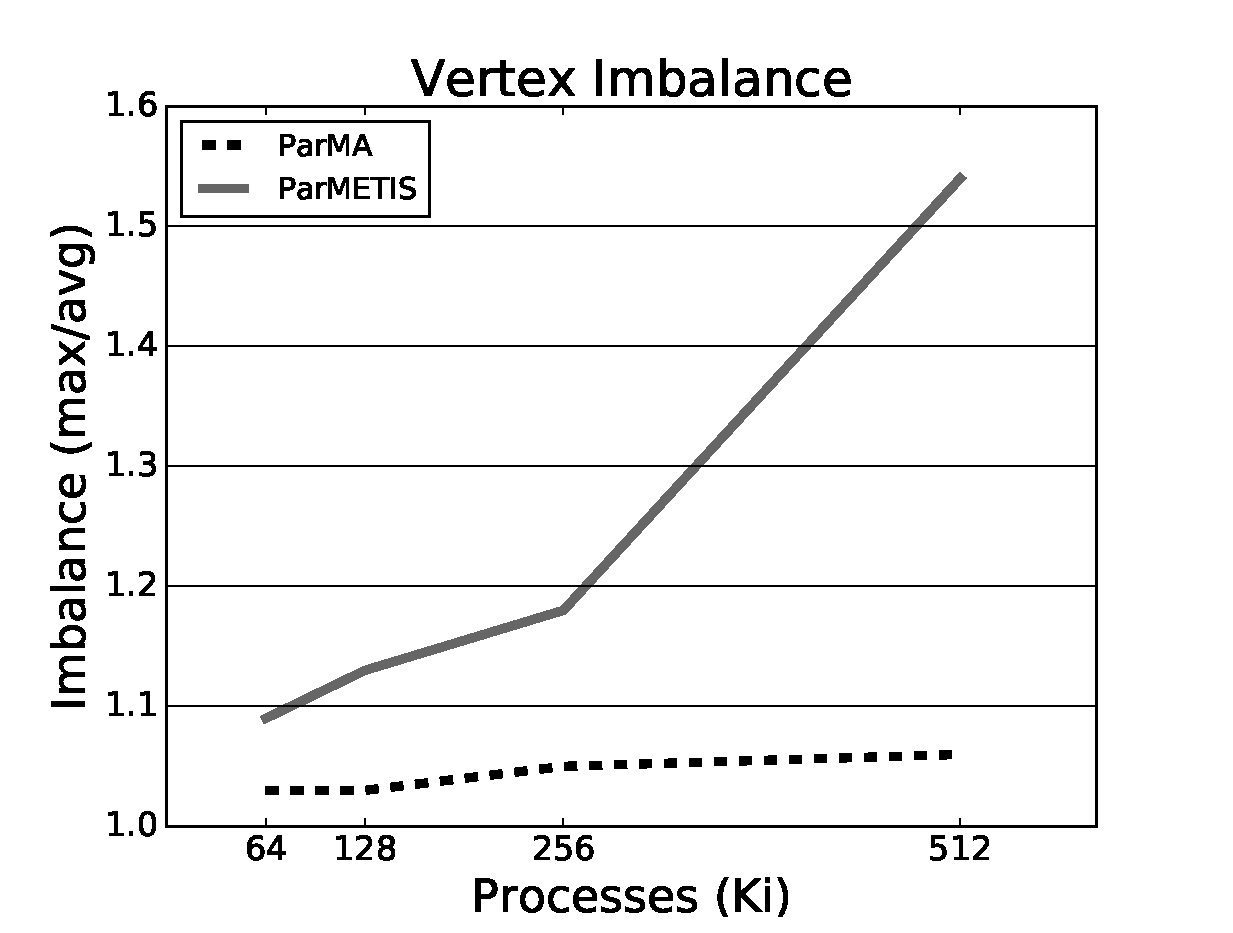
\includegraphics[width=.5\textwidth]{../parmaimprovement/results/phasta/1B/vtxImb.eps}
  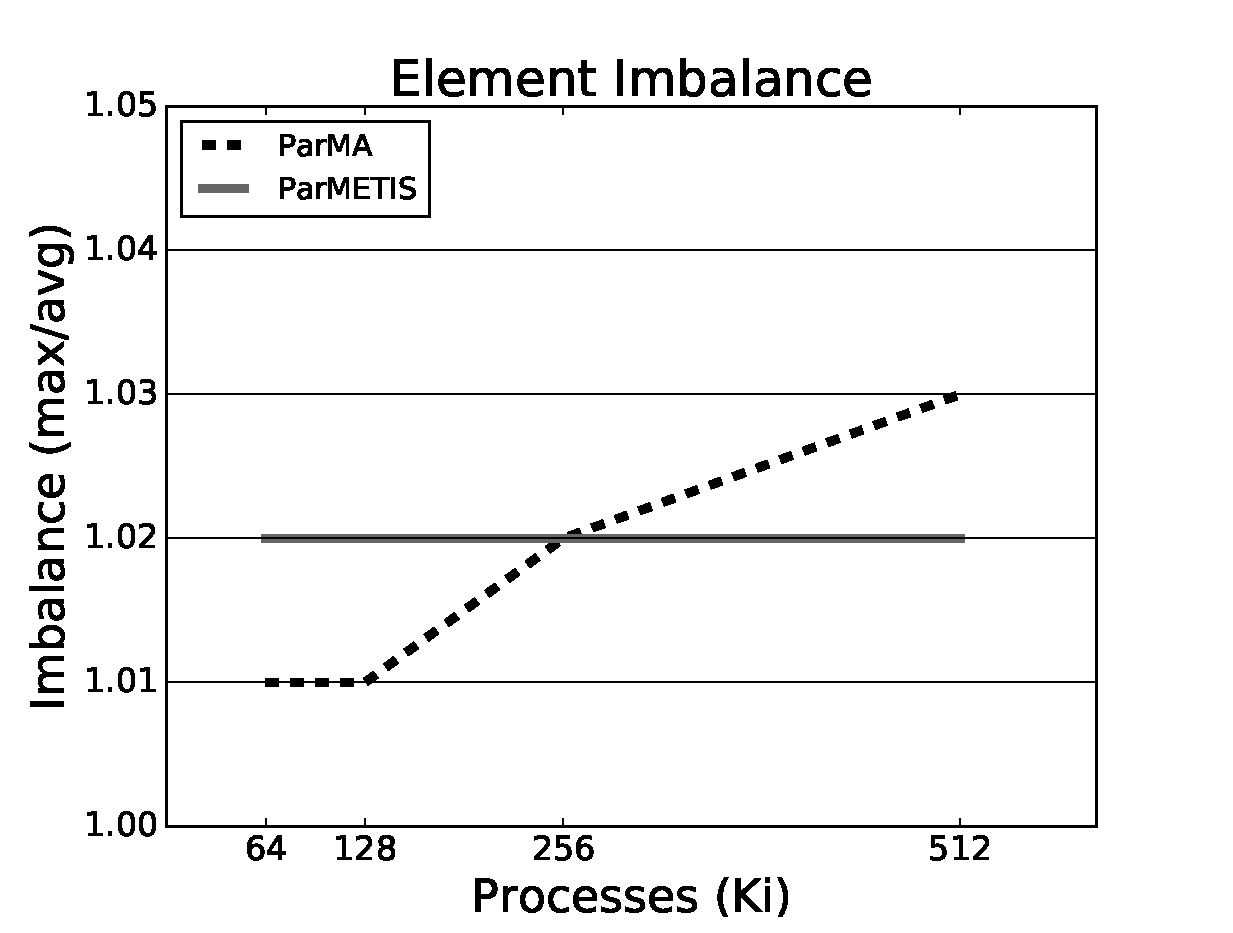
\includegraphics[width=.5\textwidth]{../parmaimprovement/results/phasta/1B/elmImb.eps}\\
  Vertex and element imbalance with and without ParMA.
\end{frame}

%----------- slide --------------------------------------------------%
\begin{frame}
  \frametitle{PHASTA Performance Improvement - Scaling}
  \centering
  At 512Ki ParMA improves the linear algebra work performance by 28\% over the
  ParMETIS partition, and improves scaling from 0.82 to 1.14 (ParMETIS 64Ki is
  the baseline).
  \centering
  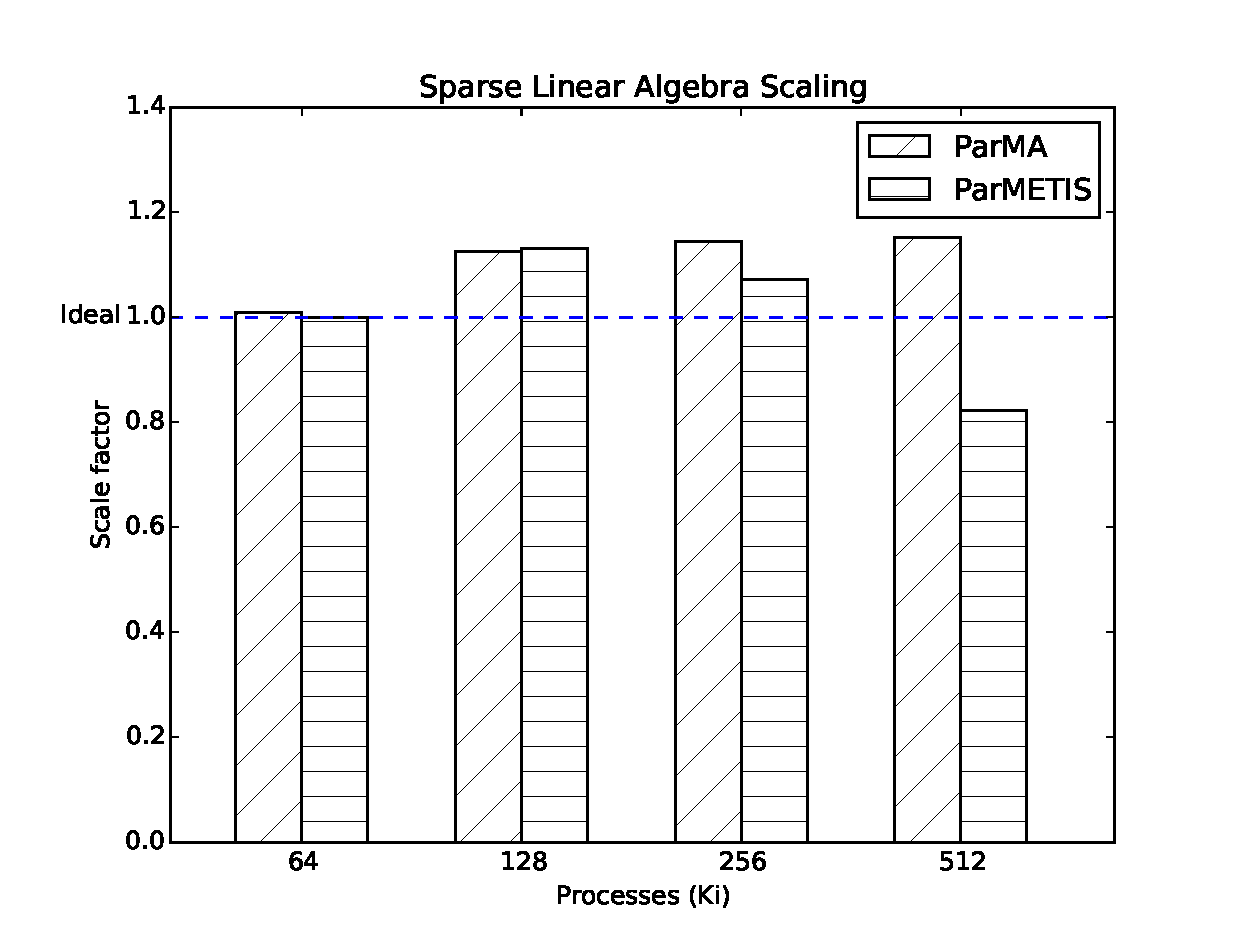
\includegraphics[width=.75\textwidth]{../parmaimprovement/results/phasta/1B/linAlgWorkScaling.eps}
\end{frame}

%----------------------------------------------------------------------%
%----------- Section --------------------------------------------------%
%----------------------------------------------------------------------%
\section{In-Memory Adaptive Workflows}
\outline

%----------- slides --------------------------------------------------%
\begin{frame}
  \frametitle{In-Memory Adaptive Workflows}
  Scalable inter-component data transfer is achieved through an in-memory
  functional coupling that avoids the high cost of filesystem access.\\
  \bigskip
  \centering
  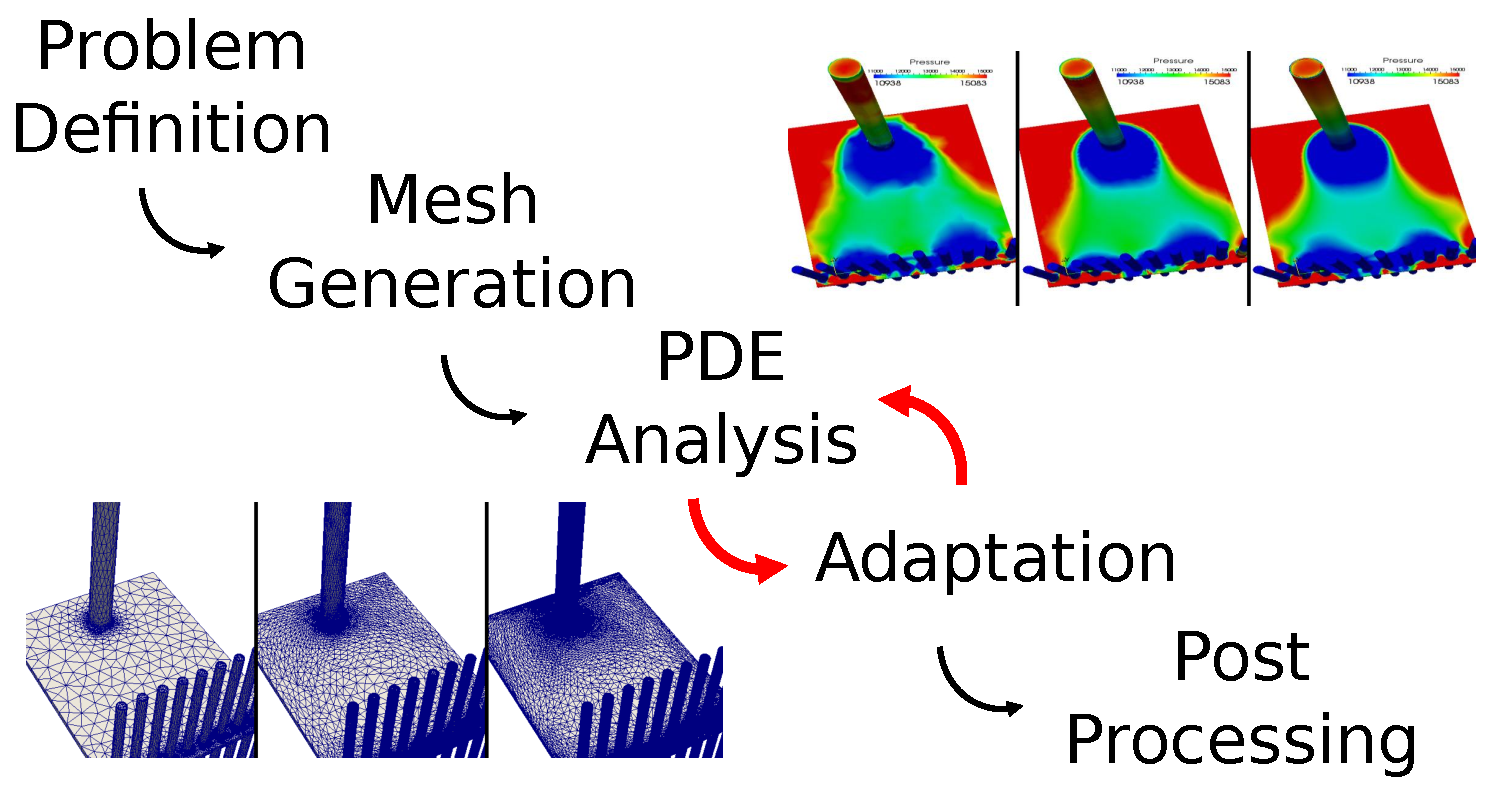
\includegraphics[width=.8\textwidth]{figs/SimulationBasedEngineeringWorkflow2.eps}
\end{frame}

%----------- slides --------------------------------------------------%
\begin{frame}
  \frametitle{Component Interactions}
  On massively parallel systems I/O dominates power consumption\\
  \smallskip
  Disk is (s)lowest in memory hierarchy\\
  \smallskip
  Bulk
  \begin{itemize}
    \item Transfer large sets of data to communicate simulation inputs/outputs
    \item Implement with files and APIs typically
    \item We replace files with in-memory data-streams to improve performance
  \end{itemize}
  Atomic
  \begin{itemize}
    \item Transfer a small set of data to communicate properties about some
      portion of the computational domain
    \item Implement with APIs
  \end{itemize}
  Alternatives
  \begin{itemize}
    \item ADIOS, GLEAN - couple executables through common file format
    \item HELIOS - framework using common interface
    \item Flatbuffers, Cap'n Proto - bulk stream-like transfers using a defined
      format
  \end{itemize}
\end{frame}

%----------- slide --------------------------------------------------%
\begin{frame}
  \frametitle{In-Memory Approaches}
  Component implementation drives coupling approach\\
  \smallskip
  Bulk data streams
  \begin{itemize}
    \item Minimal code changes
    \item Ideal for components already coupled via POSIX files
    \item Key Challenge - interface definition and memory management
  \end{itemize}
  Bulk API
  \begin{itemize}
    \item Ideal for components with APIs that support querying and modifying
      data structures
    \item Key Challenge - understanding implementation (documentation?)
  \end{itemize}
  Atomic API
  \begin{itemize}
    \item Supports common data representation and/or fine-grained operations
    \item Ideal for components with abstracted mesh and field interfaces
    \item Key Challenge - understanding implementation++
  \end{itemize}
\end{frame}

%----------- slide --------------------------------------------------%
\begin{frame}
  \frametitle{In-Memory Couplings with PUMI}
  PUMI (SCOREC)
  \begin{itemize}
    \item Anisotropic mesh adaptation with local solution transfer
    \item Dynamic load balancing via ParMA
    \item Complete mesh representation
    \item C/C++ library providing rich API
  \end{itemize}
  \bigskip
  Several C, C++, FORTRAN, and Python components have been integrated with PUMI
  to support adaptive in-memory Finite Element/Volume parallel workflows\\
  \bigskip
  Component design and data needs drive coupling decision
\end{frame}

%----------------------------------------------------------------------%
%----------- SubSection -----------------------------------------------%
%----------------------------------------------------------------------%
\subsection{PHASTA}

%----------- slide --------------------------------------------------%
\begin{frame}
  \frametitle{PHASTA In-Memory Adaptation}
  PHASTA (University of Colorado Boulder, RPI)
  \begin{itemize}
    \item Flow solver scaling to over 1Mi cores of Mira BG/Q
    \item Operates on element and vertex mesh representation
    \item Executable only - monolithic design, lots of global state
    \item Mix of Fortran 77 and 90 and C/C++
  \end{itemize}
  Coupling Approach
  \begin{itemize}
    \item Bulk data stream based coupling to reuse existing code base -
      scattered over multiple branches and groups
    \item Implement execution control APIs that stream and file-based
      execution modes
  \end{itemize}
\end{frame}

%----------- slide --------------------------------------------------%
\begin{frame}
  \frametitle{PHASTA POSIX vs. Streams - Workflow}
  First preprocessor call loads the 2Ki part mesh and partition to 4Ki, 8Ki, or 16Ki\\
  \begin{algorithm}[H]
    \caption{Two-phase PHASTA-chef Adaptive Loop}\label{alg:twophase}
    \small
    \begin{algorithmic}[1]
      \Procedure{adaptiveLoop}{$max\_steps$}
        \State $pumi\_mesh \gets$ load the partitioned PUMI mesh
               from disk\label{step:loadmesh}
        \State $geom \gets$ load the geometric model from
               disk\label{step:loadgeom}
        \State $chef\_probdef \gets$ load the chef problem definition
               from disk\label{step:loadprobdef}
        \State \Call{preprocessor}{$pumi\_mesh$,$geom$,$chef\_probdef$}
        \State $step\_number \gets$ 0
        \While{$step\_number < max\_steps$\label{step:loop}}
          \State $step\_number \gets$ \Call{PHASTA}{$N$}
          \State \Call{readAndAttach}{$size\_field$,$phasta\_fields$,$pumi\_mesh$}
          \State \Call{meshadapt}{$pumi\_mesh$,$size\_field$,$max\_iterations$}
          \State \Call{preprocessor}{$pumi\_mesh$,$geom$,$chef\_probdef$}
        \EndWhile
      \EndProcedure
    \end{algorithmic}
  \end{algorithm}
\end{frame}

\begin{frame}
  \frametitle{PHASTA POSIX vs. Streams}
  Test case
  \begin{itemize}
    \item Dambreak - released column of water flows to the right
    \item 124M elements
    \item Intel Knights Landing (KNL) based Theta Cray XC40 system at
      the Argonne Leadership Computing Facility (ALCF) using 64
      processes per-node
    \item KNL in cache-quad mode
    \item data-streams vs. ramdisk (DRAM) vs. POSIX GPFS vs. POSIX Lustre
  \end{itemize}
  \centering
  \includemedia[
    activate=pageopen,
    addresource=animations/dambreak540pLow.mov,
    flashvars={%
       src=animations/dambreak540pLow.mov
      &autoPlay=true
      &loop=true
      &scaleMode=stretch
    }
  ]{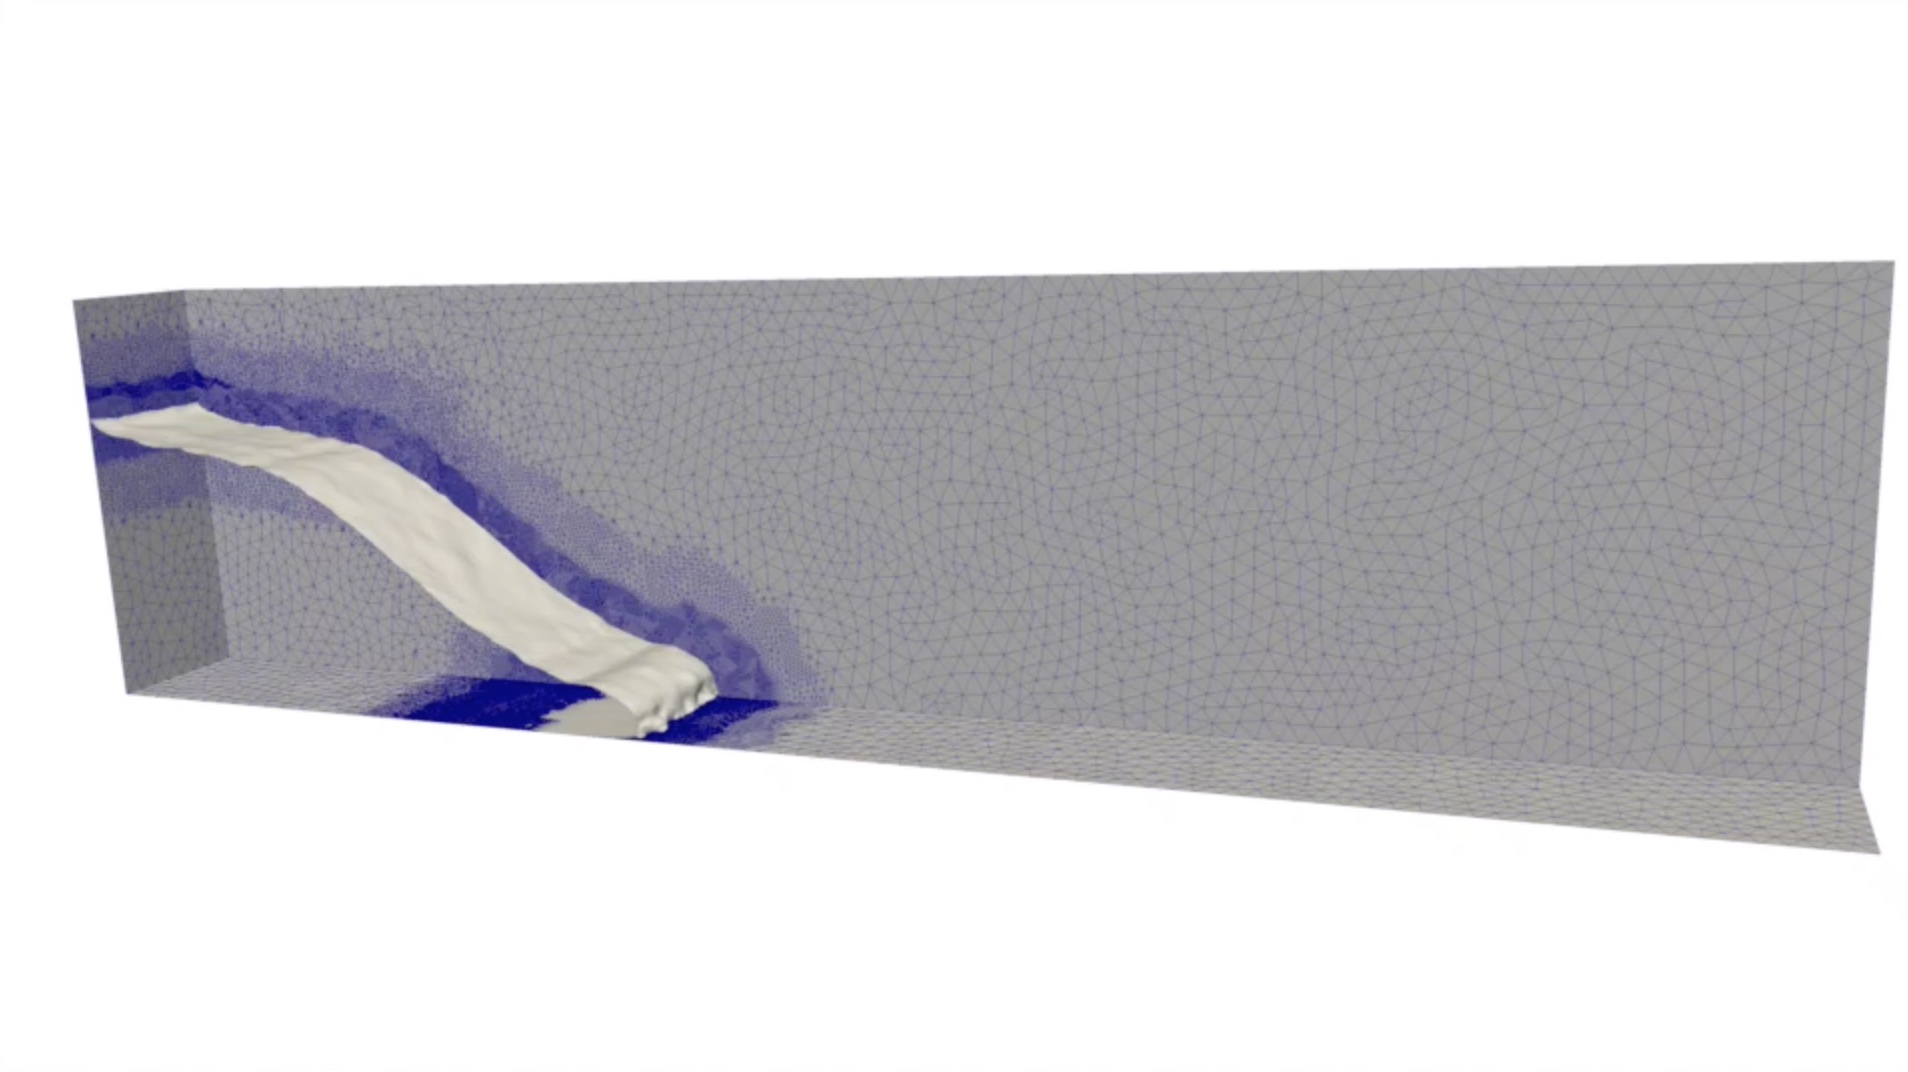
\includegraphics[width=.55\textwidth]{animations/dambreak540pLow.jpeg}}{StrobeMediaPlayback.swf}\\
  \tiny
  PHASTA in-memory adaptive dambreak simulation
\end{frame}

%----------- slide --------------------------------------------------%
\begin{frame}
  \frametitle{PHASTA Results - chef Transfer Sizes}
  The number of bytes read/written at each cycle is the same
  \begin{itemize}
    \item chef pre-process - no mesh topology changes
    \item PHASTA solver does not advance the flow field - work stays constant
  \end{itemize}
  Each I/O method reads/writes the same number of bytes at each process count
  \begin{itemize}
    \item ParMA balancing is deterministic
  \end{itemize}
  \centering
  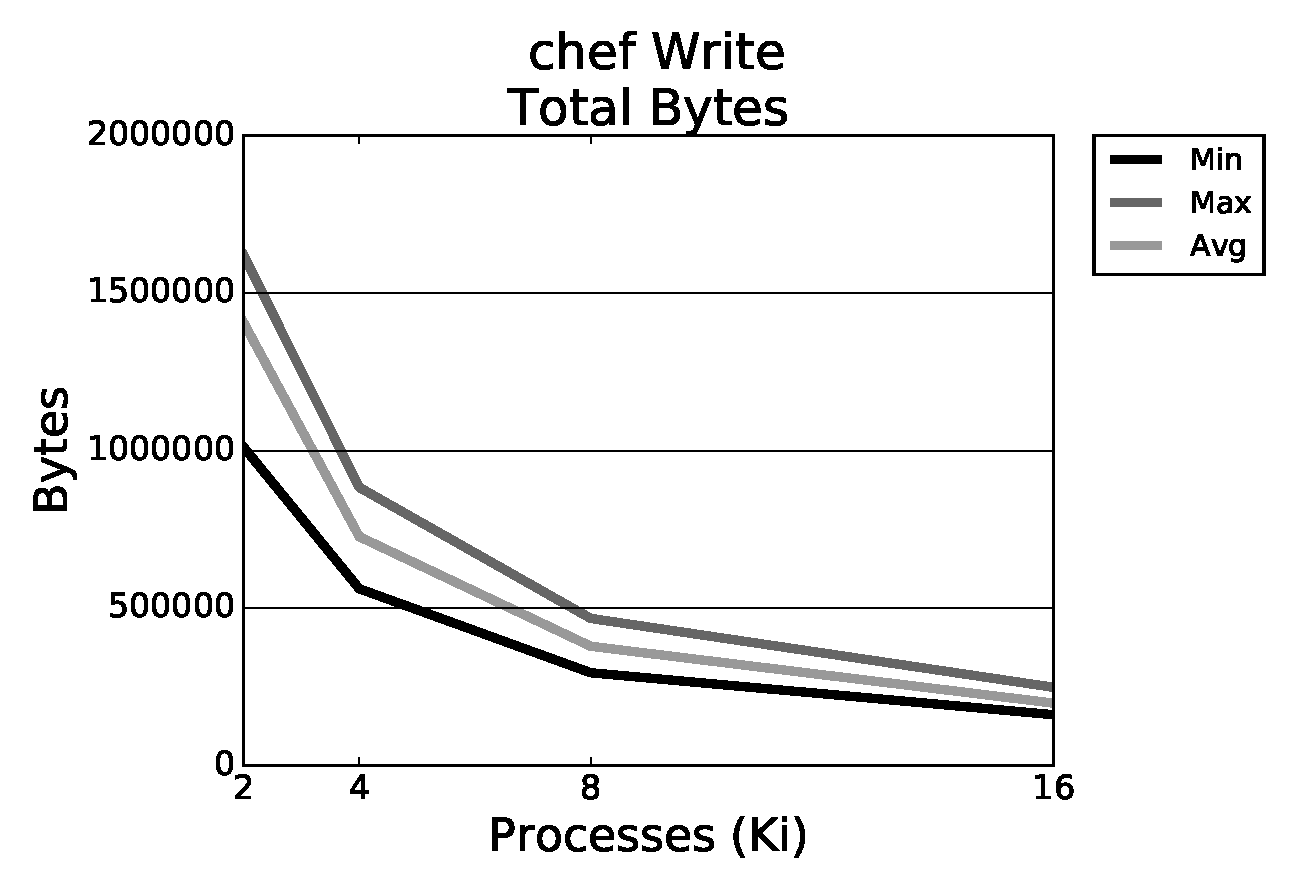
\includegraphics[width=.45\textwidth]{../imp/results/phasta-dambreak/theta/streamchefWriteTotalBytes.eps}
  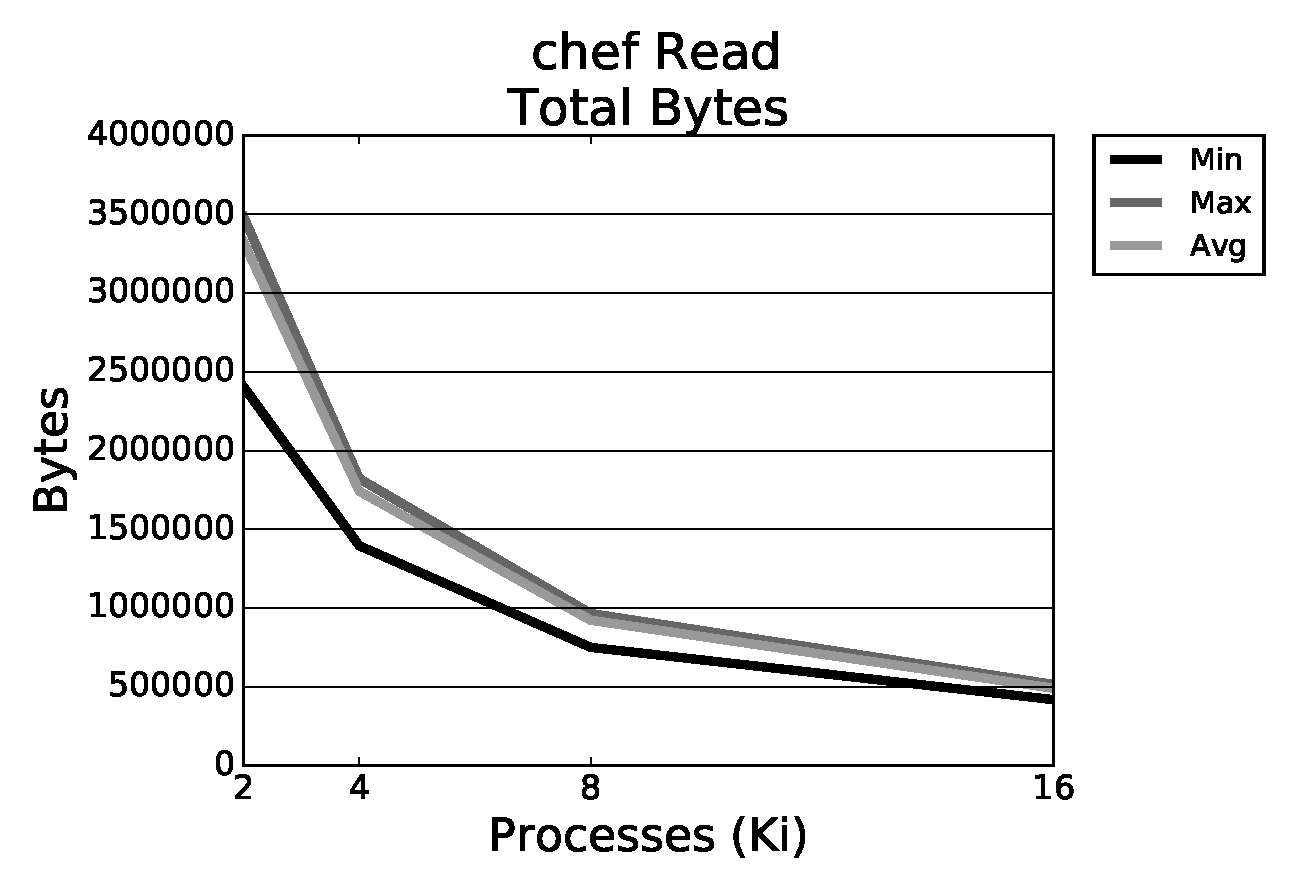
\includegraphics[width=.45\textwidth]{../imp/results/phasta-dambreak/theta/streamchefReadTotalBytes.eps}\\
  chef total bytes read and written per-process. PHASTA reads(writes) the same number of
  bytes that chef wrote(reads).
\end{frame}

%----------- slide --------------------------------------------------%
\begin{frame}
  \frametitle{PHASTA Results - Read/Write}
  \begin{itemize}
    \item More than an order of magnitude performance improvement of the in-memory
      transfer versus POSIX file-based transfer
    \item In-memory transfer is embarrassingly parallel - strong scaling
  \end{itemize}
  \centering
  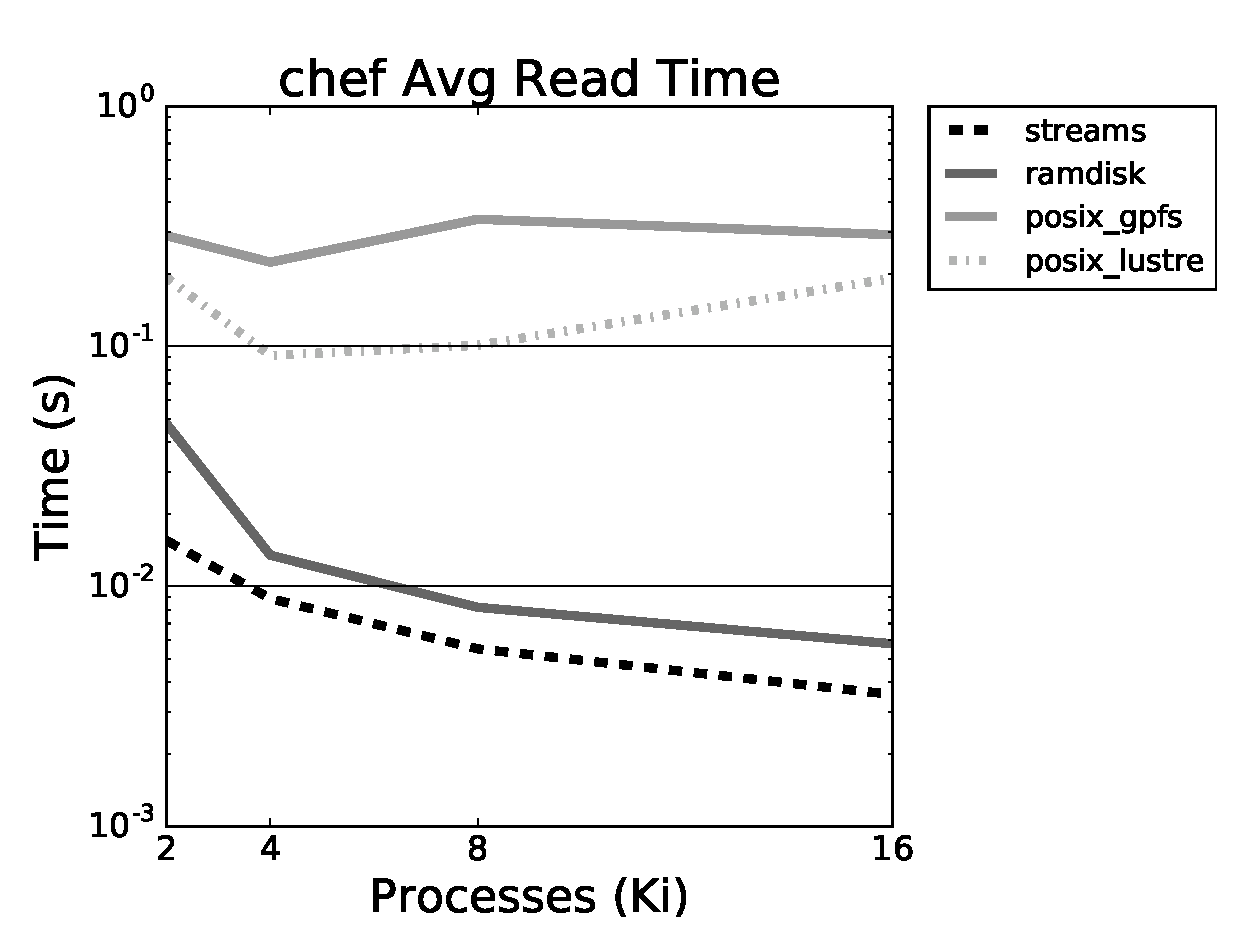
\includegraphics[width=0.45\textwidth]{../imp/results/phasta-dambreak/theta/chefreadavg.eps}
  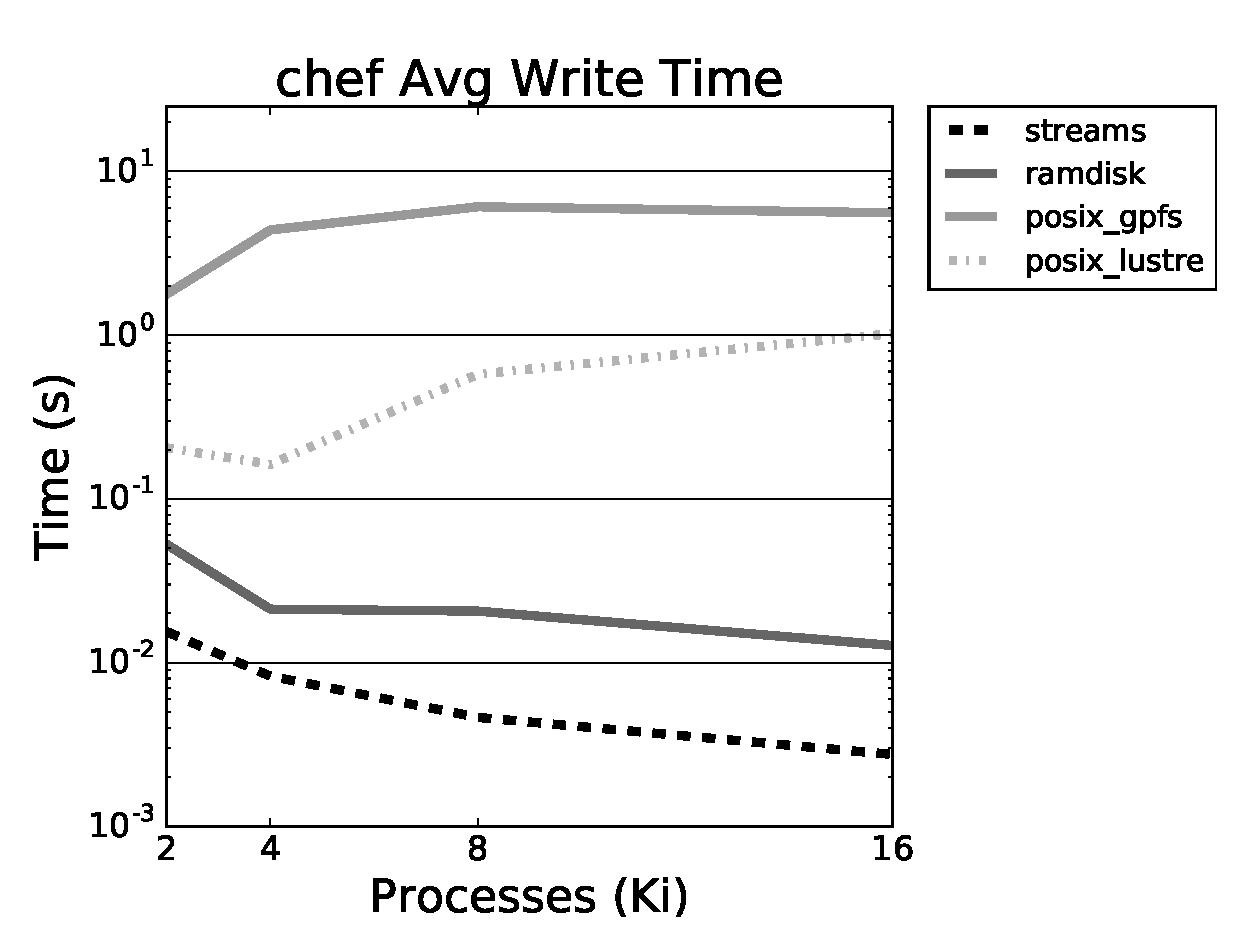
\includegraphics[width=0.45\textwidth]{../imp/results/phasta-dambreak/theta/chefwriteavg.eps}\\
  chef streams, ramdisk, and POSIX average read and write time on ALCF Theta.
\end{frame}

%----------- slide --------------------------------------------------%
\begin{frame}
  \frametitle{PHASTA Results - Per-cycle Read Time}
  \centering
  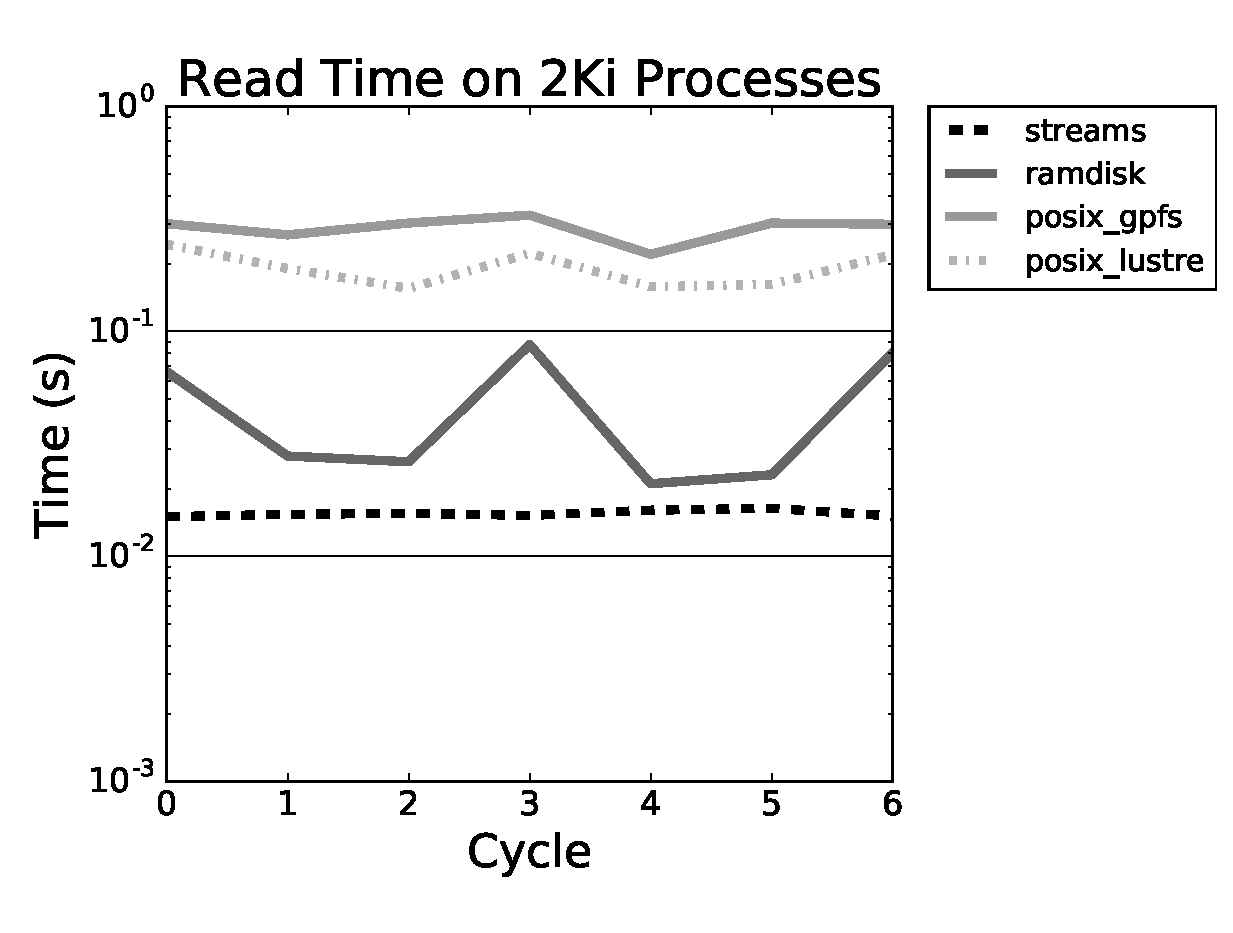
\includegraphics[width=0.45\textwidth]{../imp/results/phasta-dambreak/theta/chef2048read.eps}
  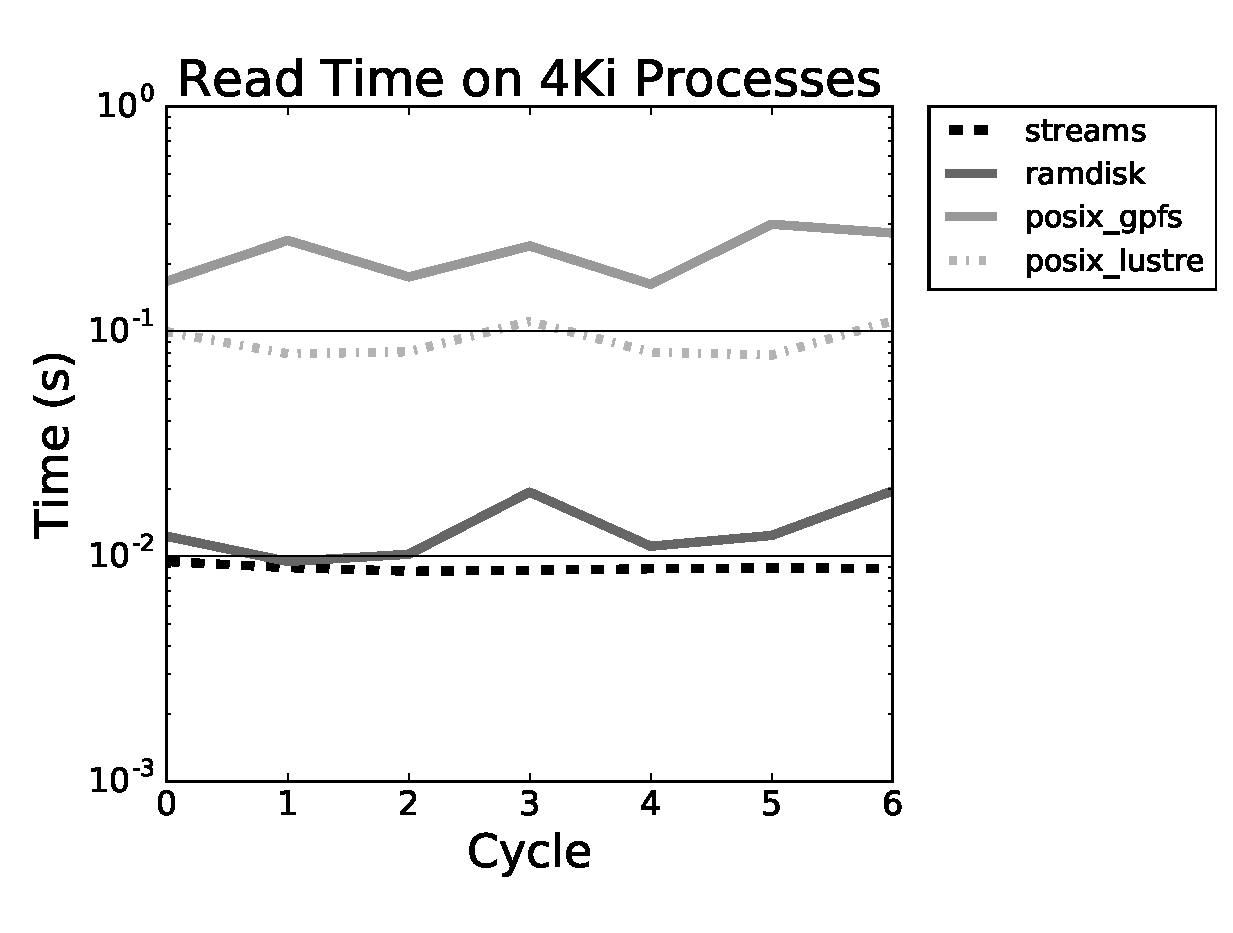
\includegraphics[width=0.45\textwidth]{../imp/results/phasta-dambreak/theta/chef4096read.eps}\\
  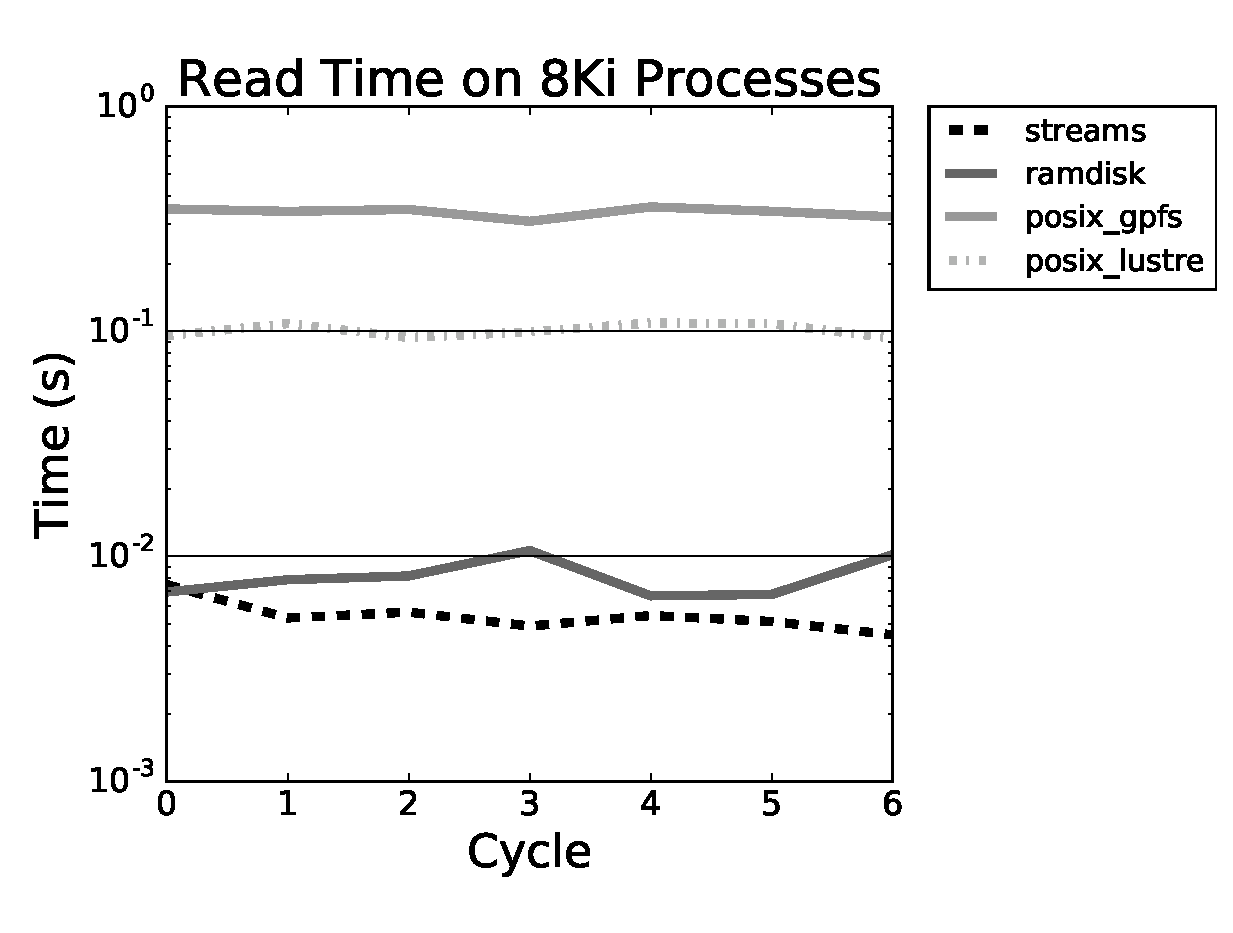
\includegraphics[width=0.45\textwidth]{../imp/results/phasta-dambreak/theta/chef8192read.eps}
  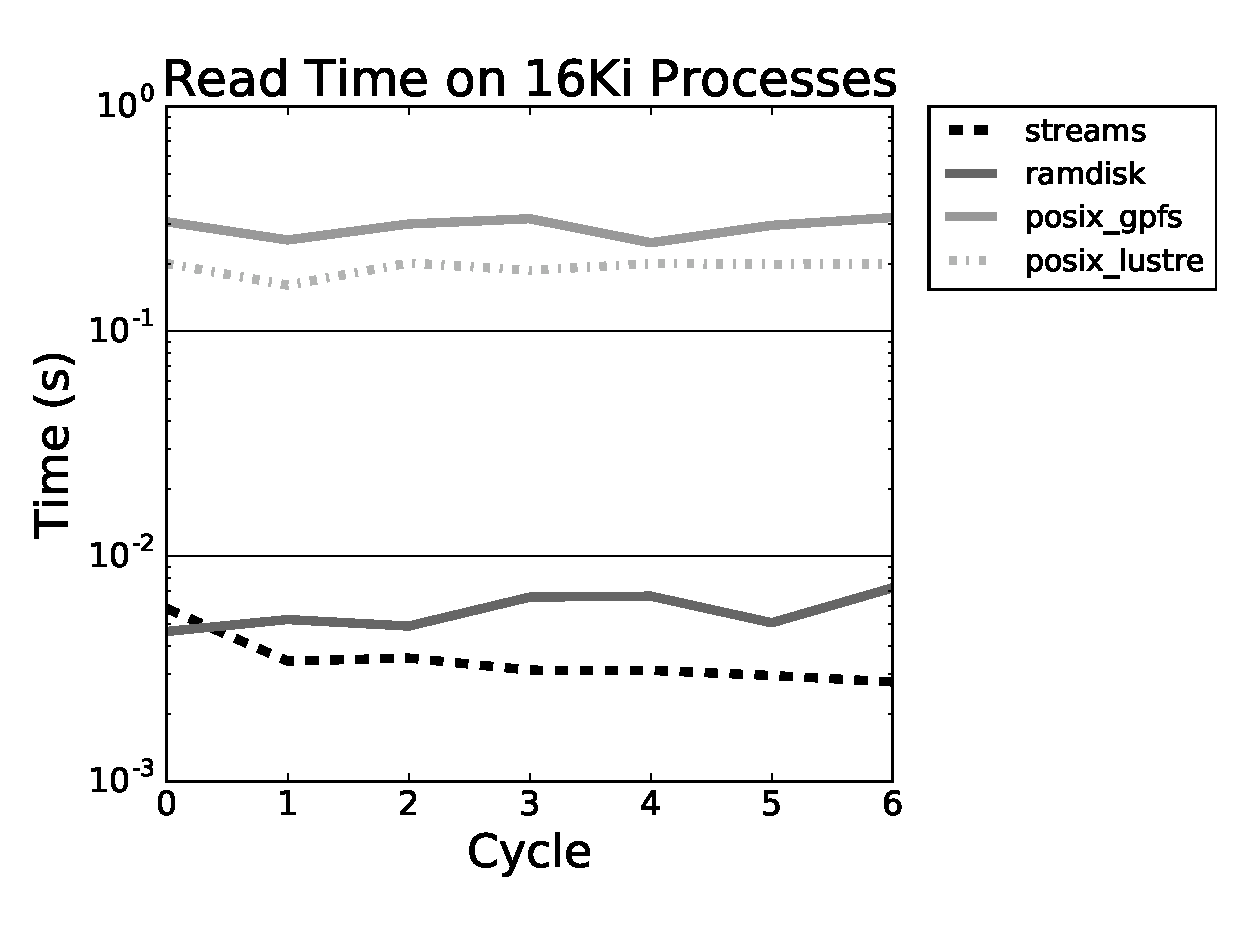
\includegraphics[width=0.45\textwidth]{../imp/results/phasta-dambreak/theta/chef16384read.eps}\\
\end{frame}

%----------- slide --------------------------------------------------%
\begin{frame}
  \frametitle{PHASTA Results - Per-cycle Write Time}
  \centering
  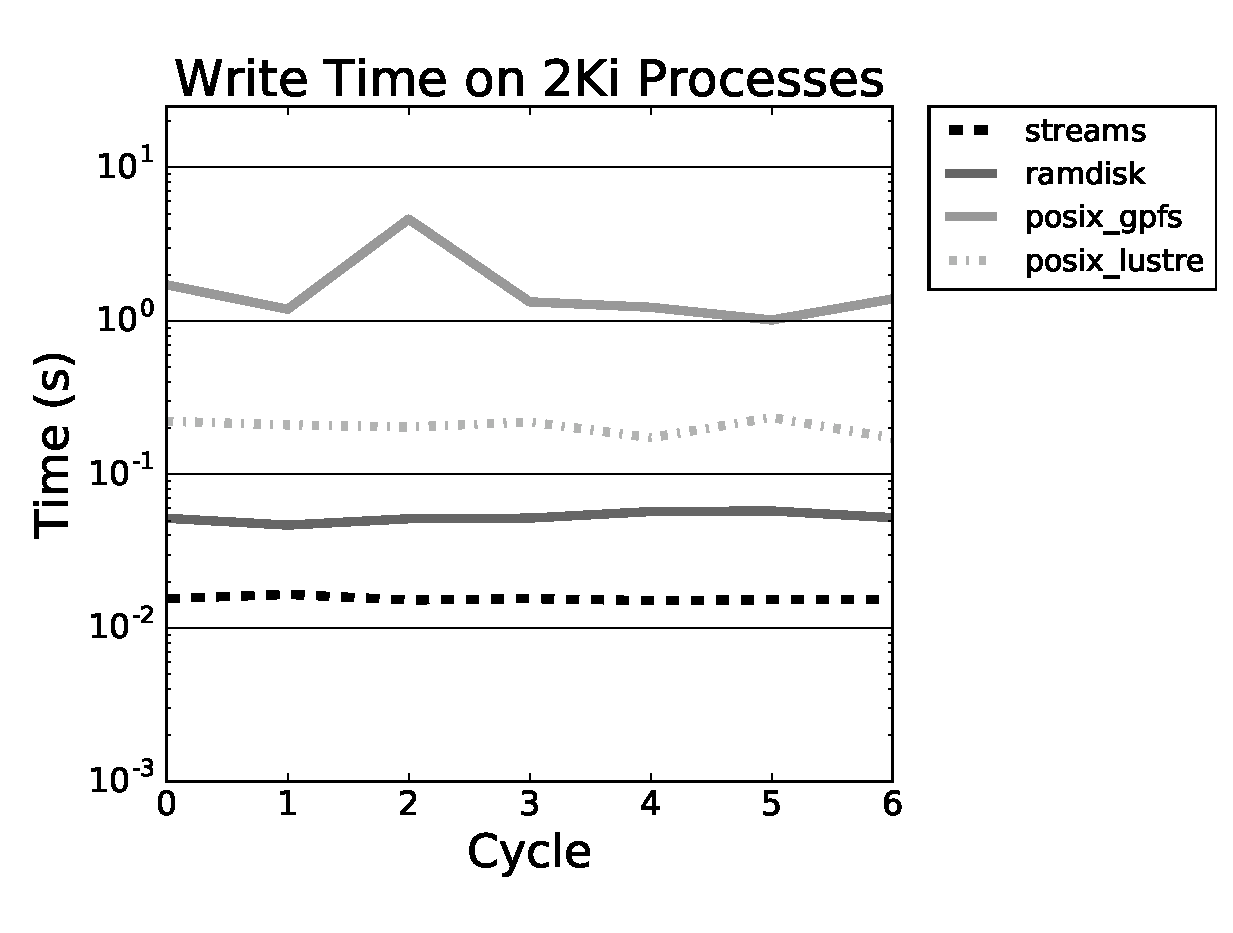
\includegraphics[width=0.45\textwidth]{../imp/results/phasta-dambreak/theta/chef2048write.eps}
  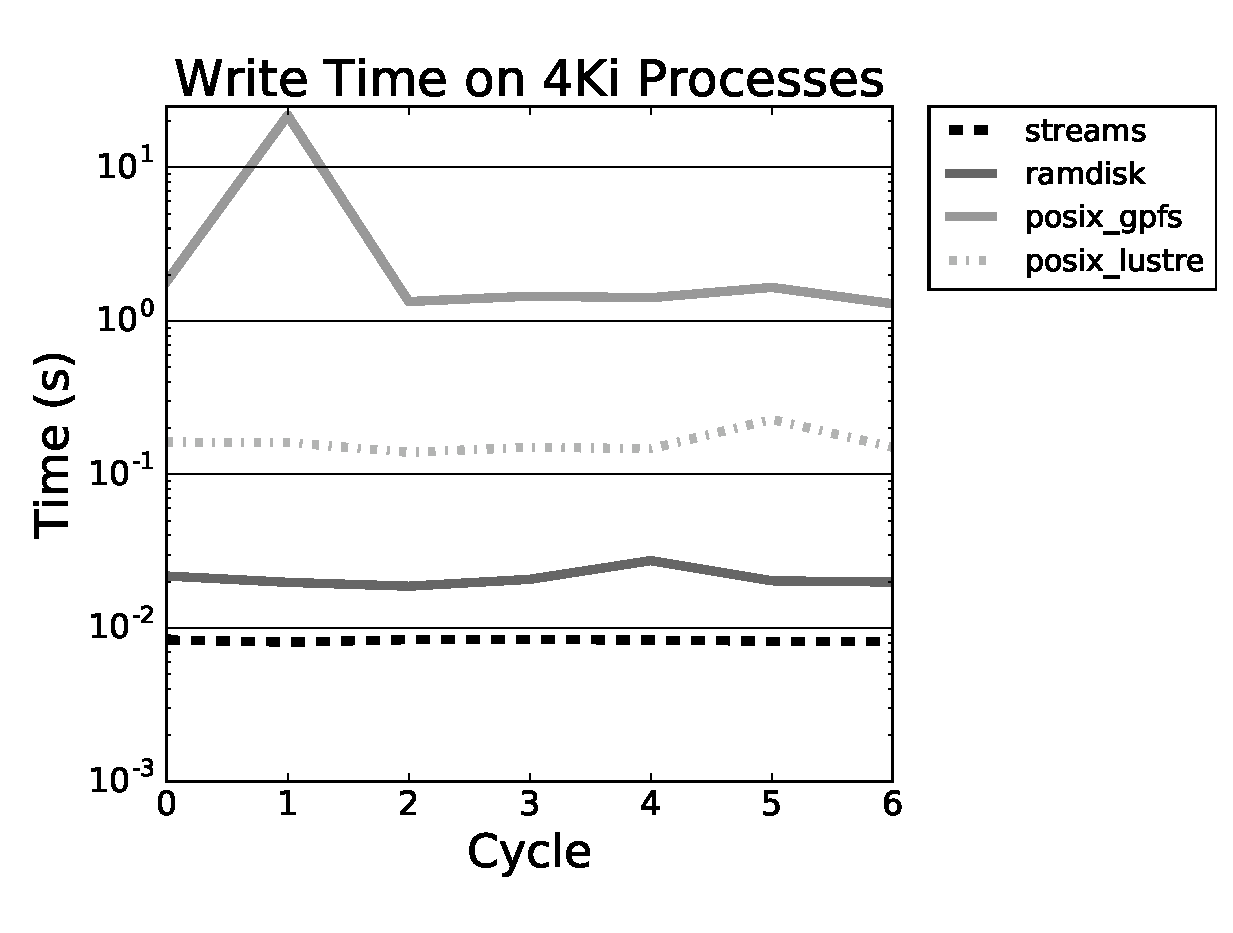
\includegraphics[width=0.45\textwidth]{../imp/results/phasta-dambreak/theta/chef4096write.eps}\\
  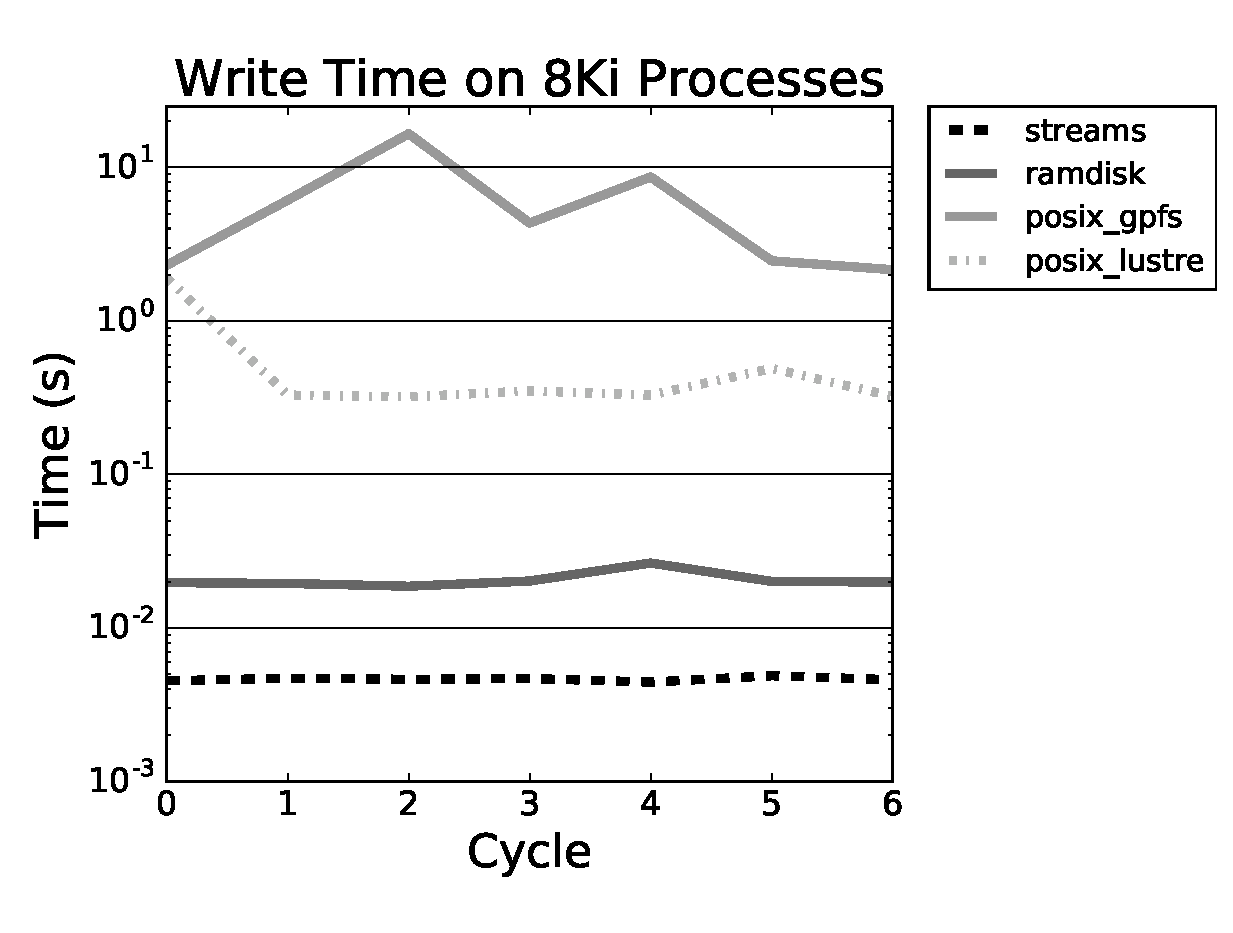
\includegraphics[width=0.45\textwidth]{../imp/results/phasta-dambreak/theta/chef8192write.eps}
  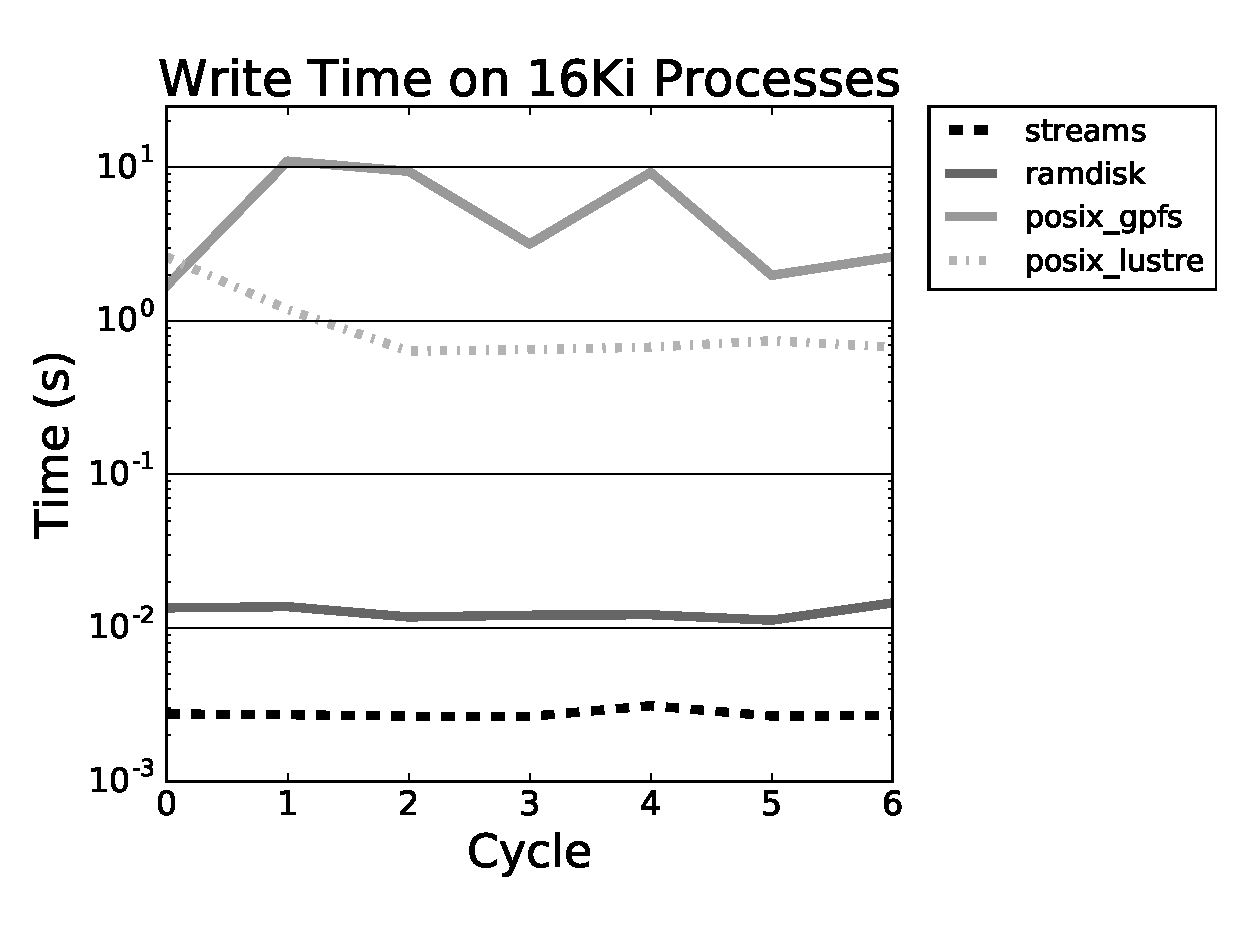
\includegraphics[width=0.45\textwidth]{../imp/results/phasta-dambreak/theta/chef16384write.eps}\\
\end{frame}

%----------------------------------------------------------------------%
%----------- SubSection -----------------------------------------------%
%----------------------------------------------------------------------%
\subsection{Albany}

\begin{frame}
  \frametitle{Albany}
  Albany (Sandia National Laboratories)
  \begin{itemize}
    \item C/C++, modular design, APIs, no existing file based coupling
    \item Uses many of the C++ Trilinos packages
  \end{itemize}
  Coupling Approach
  \begin{itemize}
    \item Define bulk transfers of field and mesh connectivity via APIs
  \end{itemize}
  \centering
  \includegraphics[width=0.6\textwidth]{../imp/figures/albany.png}\\
  \small
  Albany's template-based component interactions~\cite{albany2016}.
\end{frame}

%----------- slide --------------------------------------------------%
\begin{frame}
  \frametitle{Albany Workflow}
  \begin{algorithm}[H]
    \caption{Albany-PUMI Adaptive Loop}
    \small
    \begin{algorithmic}[1]
      \Procedure{adaptiveLoop}{$max\_steps$}
        \State $pumi\_mesh \gets$ load the partitioned PUMI mesh from disk
        \State $geom \gets$ load the geometric model from disk
        \State $probdef \gets$ load the Albany problem definition from disk
        \State \Call{createConnectivity}{$pumi\_mesh$} 
        \State \Call{createNodeAndSideSets}{$pumi\_mesh$,$probdef$} 
        \State $step\_number \gets$ 0
        \While{$step\_number < max\_steps$}
          \State \Call{solveLoadStep}{$step\_number$++}
          \State \Call{getFields}{$pumi\_mesh$} 
          \State $size\_field \gets$ \Call{SPR}{$pumi\_mesh$}
          \State \Call{MeshAdapt}{$pumi\_mesh$,$size\_field$}
          \State \Call{ParMA}{vtx$>$elm,$pumi\_mesh$}
          \State \Call{createConnectivity}{$pumi\_mesh$} 
          \State \Call{createNodeAndSideSets}{$pumi\_mesh$,$probdef$} 
          \State \Call{setFields}{$pumi\_mesh$} 
        \EndWhile
      \EndProcedure
    \end{algorithmic}
  \end{algorithm}
\end{frame}

%----------- slide --------------------------------------------------%
\begin{frame}
  \frametitle{Albany Thermal Creep and Large Deformation}
  \centering
  \includegraphics[width=0.45\textwidth]{../imp/results/albany/8M_9_adapt_eb.075/figs/t2-crinkle-zoom.eps}
  \includegraphics[width=0.45\textwidth]{../imp/results/albany/8M_9_adapt_eb.075/figs/t5-crinkle-zoom.eps}\\
  \small
  3x3 solderball mesh after four adaptation cycles.\\
  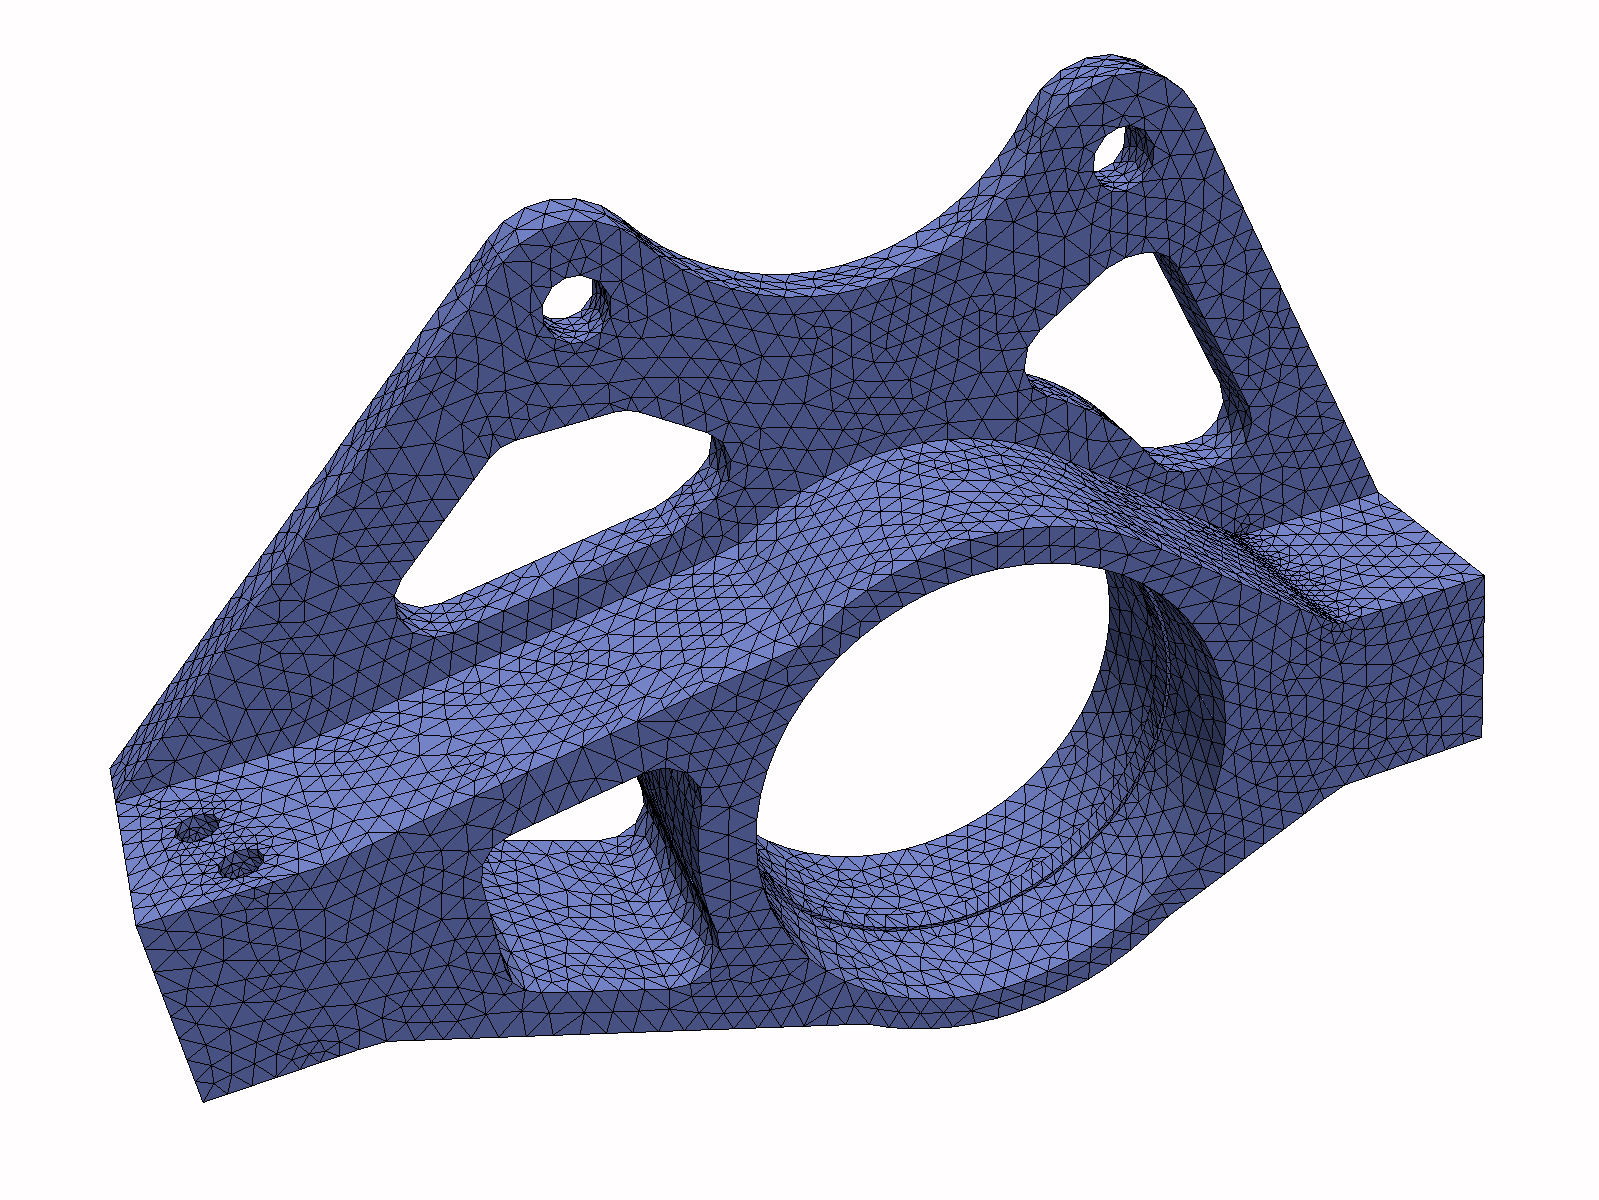
\includegraphics[width=.45\textwidth]{../imp/figures/upright/upright-initial.png}
  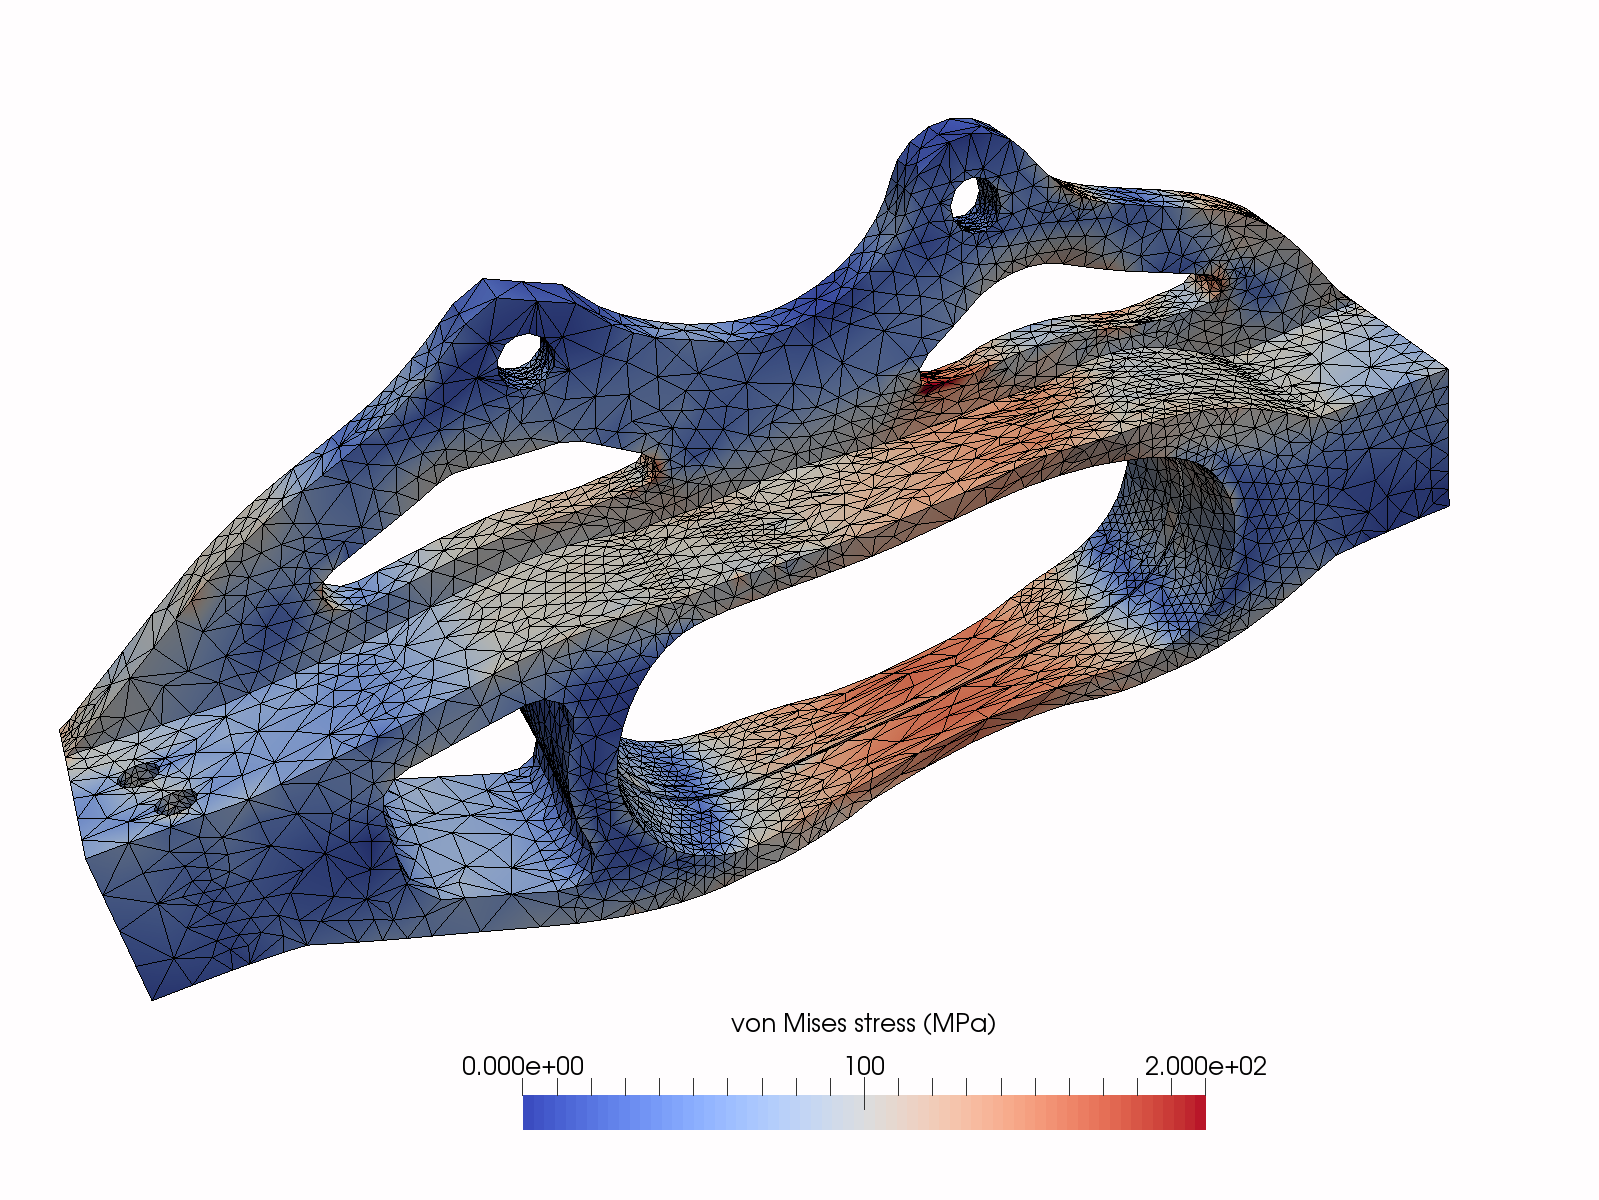
\includegraphics[width=.45\textwidth]{../imp/figures/upright/upright-final.png}\\
  \small
  Large deformation of the RPI Formula Hybrid suspension upright.
\end{frame}

%----------------------------------------------------------------------%
%----------- SubSection -----------------------------------------------%
%----------------------------------------------------------------------%
\subsection{Omega3P}

\begin{frame}
  \frametitle{Omega3P}
  ACE3P (SLAC National Accelerator Laboratory)
  \begin{itemize}
    \item C/C++, modular design, APIs, no existing file based coupling
    \item Depends on many `native' components with templated interfaces
      (e.g., the DistMesh)
  \end{itemize}
  Coupling Approach
  \begin{itemize}
    \item Support high order meshes and geometry via PUMI APIs for bulk and
      atomic transfers
    \item Use two copies of the mesh - PUMI and DistMesh
  \end{itemize}
\end{frame}

%----------- slide --------------------------------------------------%
\begin{frame}
  \frametitle{Omega3P Workflow}
  \begin{algorithm}[H]
    \caption{Omega3P-PUMI Adaptive Loop}\label{alg:omega3pAdaptLoop}
    \begin{algorithmic}[1]
      \Procedure{adaptiveLoop}{$max\_steps$}
        \State $pumi\_mesh \gets$ load the partitioned PUMI mesh from disk
        \State $geom \gets$ load the geometric model from disk
        \State $probdef \gets$ load the Omega3P problem definition from disk
        \State $dist\_mesh \gets$ \Call{createDistMesh}{$pumi\_mesh$} \Comment{{\tiny bulk}}
        \While{ not ($converged \gets$ \Call{eigenSolver}{$dist\_mesh$}) } \Comment{{\tiny atomic}}
          \State \Call{getElectricField}{$pumi\_mesh$} \Comment{{\tiny bulk}}
          \State \Call{destroy}{$dist\_mesh$}
          \State $size\_field \gets$ \Call{SPR}{$pumi\_mesh$}
          \State \Call{MeshAdapt}{$pumi\_mesh$,$size\_field$}
          \State \Call{ParmaGhost}{edge$=$face$>$rgn,$pumi\_mesh$} \Comment{{\tiny quadratic Nedelec}}
          \State $dist\_mesh \gets$ \Call{createDistMesh}{$pumi\_mesh$} \Comment{{\tiny bulk}}
        \EndWhile
      \EndProcedure
    \end{algorithmic}
  \end{algorithm}
\end{frame}

%----------- slide --------------------------------------------------%
\begin{frame}
  \frametitle{Omega3P - Atomic transfer}
  \begin{algorithm}[H]
    \caption{Jacobian Calculation for Matrix Assembly}
    \label{alg:omega3pJacobian}
    \begin{algorithmic}[1]
      \State // loop over DistMesh elements
      \ForAll{ $M^3_i \in M$ }
      \State $pumiElementPtr \gets getPumiElementPtr(M^3_i)$
             \label{alg:o3p_pointer}
      \ForAll{ integration points }
        \State $xi \leftarrow$ getBaryCentricCoords(integration point)
               \label{alg:o3p_bary}
        \State \texttt{apf::Matrix3x3} $J$
        \State \texttt{apf::getJacobian($pumiElementPtr$,$xi$,$J$)}
               \label{alg:o3p_getJ}
        \State // complete element matrix computation
      \EndFor
      \State // insert element matrix contributions into stiffness matrix
      \EndFor
    \end{algorithmic}
  \end{algorithm}
\end{frame}

%----------- slide --------------------------------------------------%
\begin{frame}
  \frametitle{Omega3P Adaptation}
  \centering
  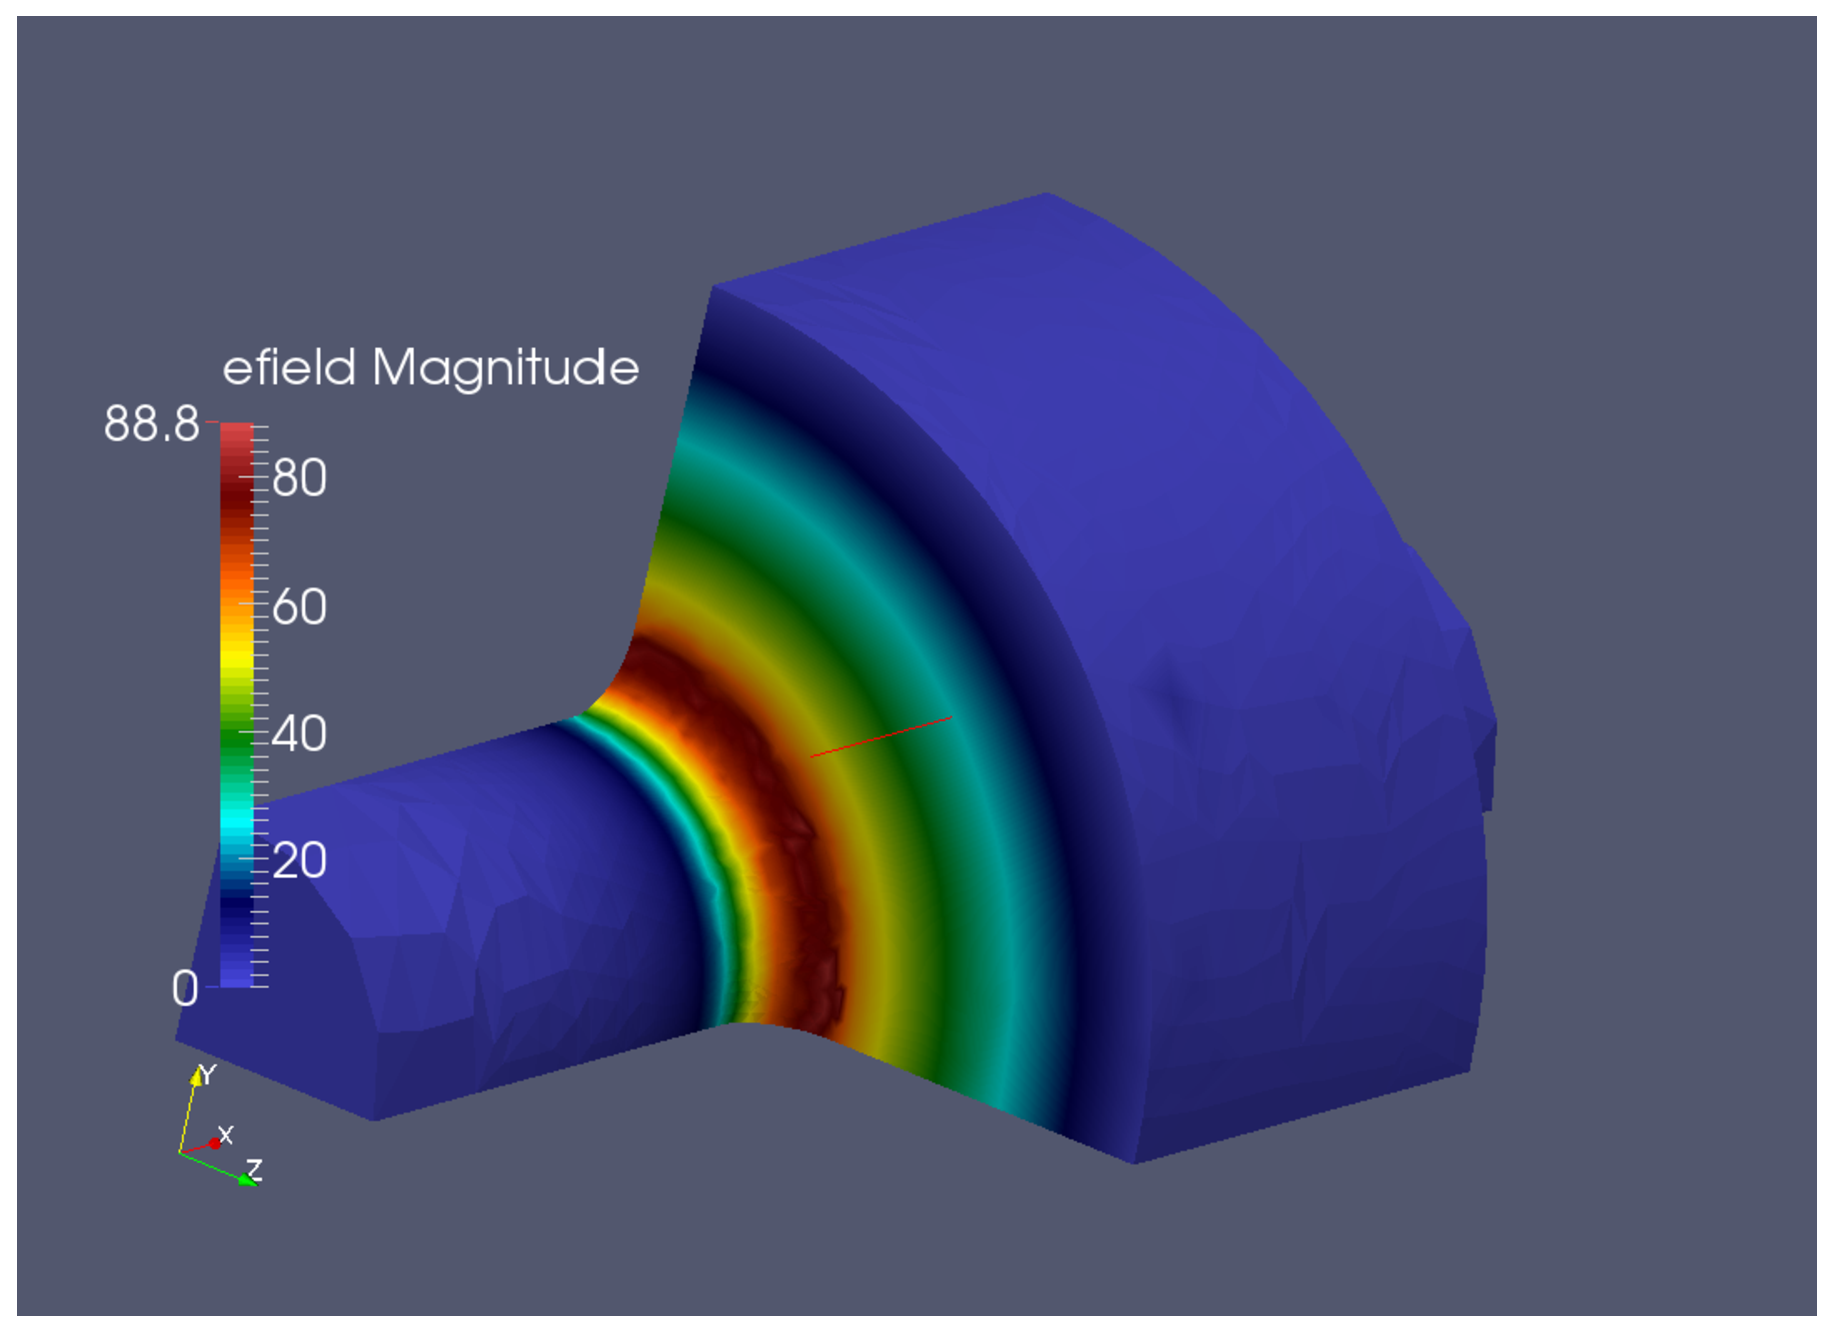
\includegraphics[width=0.43\textwidth]{../imp/figures/omega3p/pillbox_al_3_ar_0p0125_14221_elems_e_field.eps}
  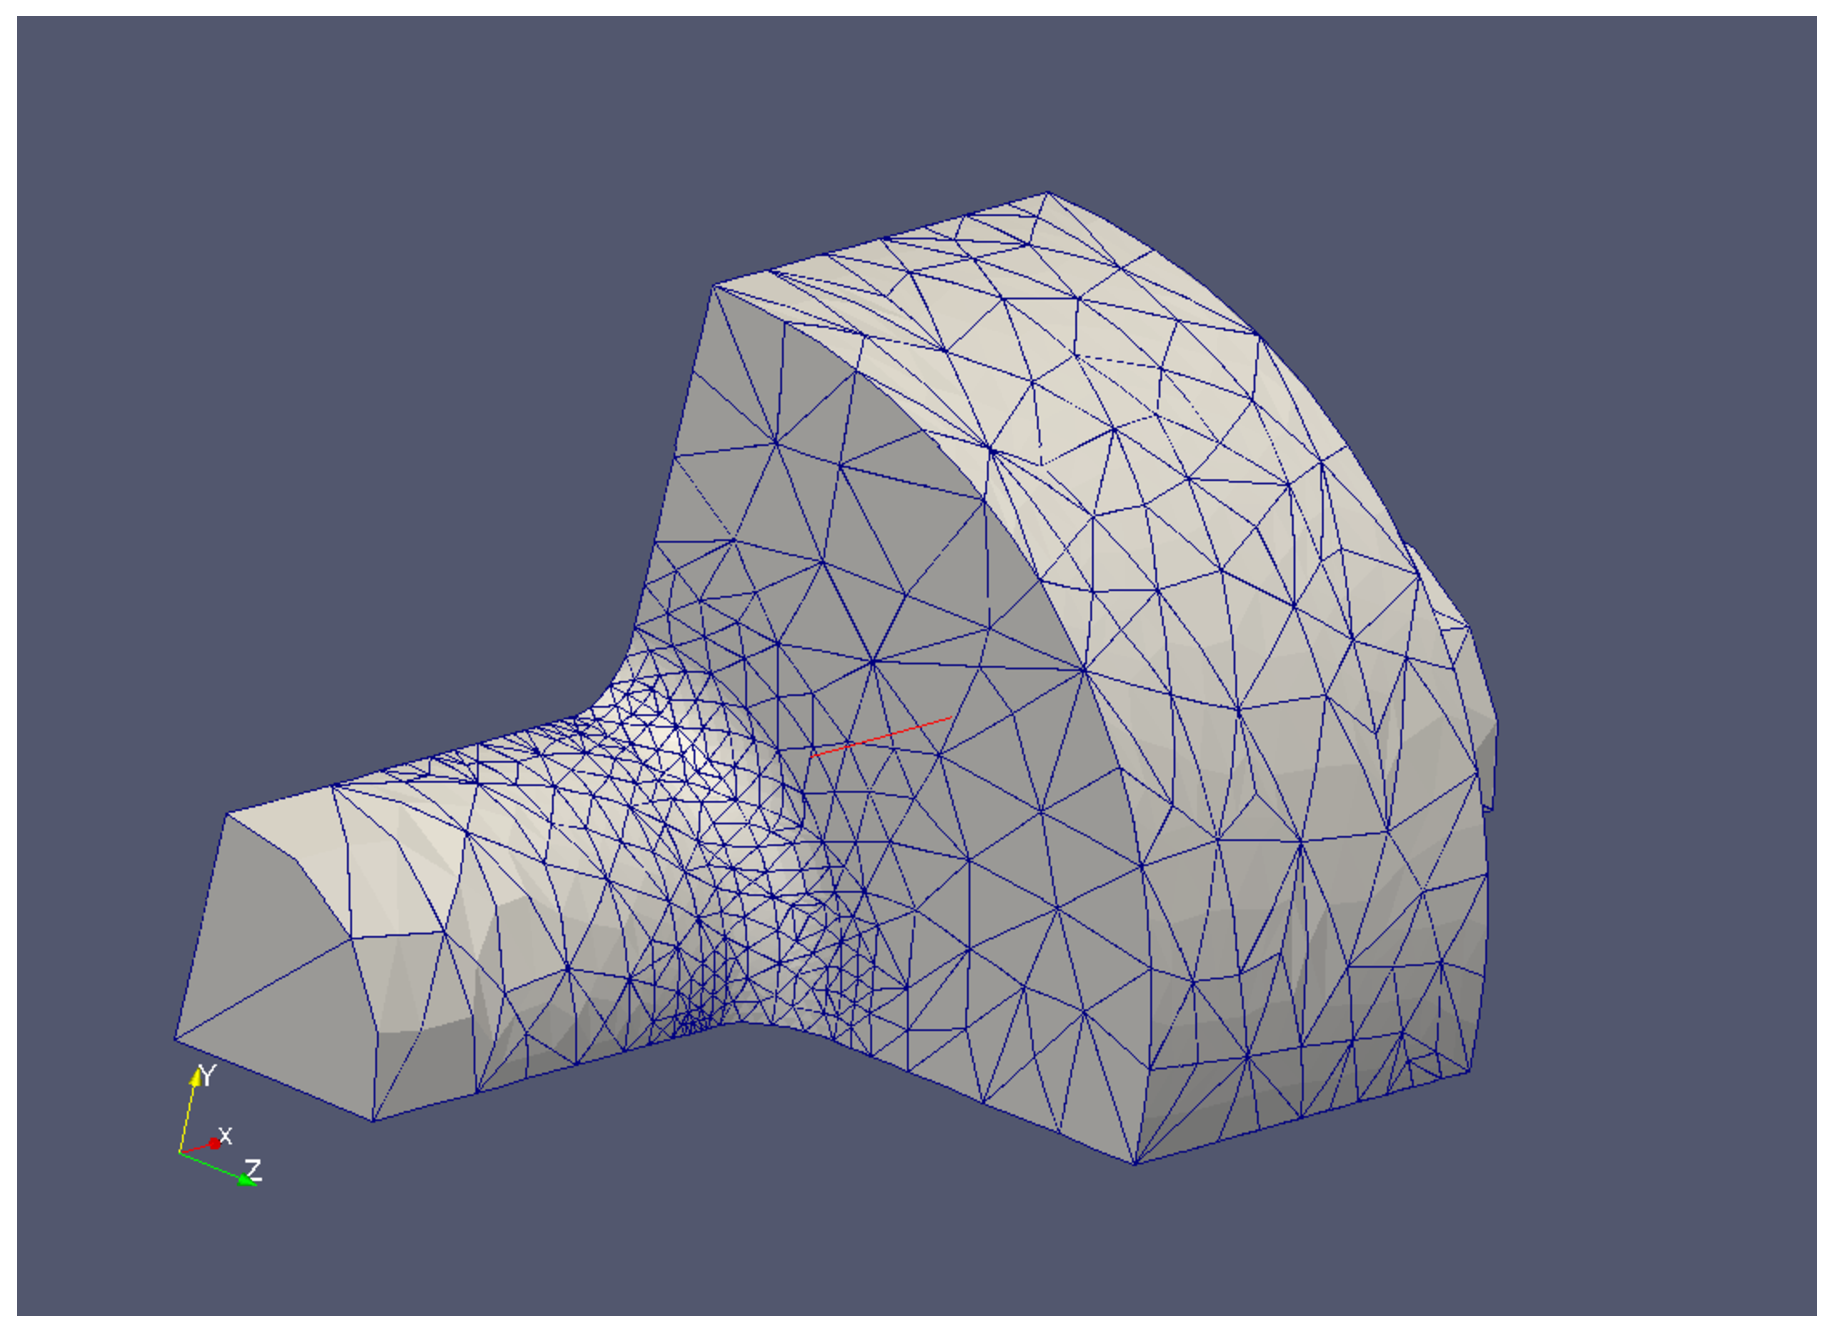
\includegraphics[width=0.43\textwidth]{../imp/figures/omega3p/pillbox_al_3_ar_0p0125_14221_elems_mesh.eps}\\
  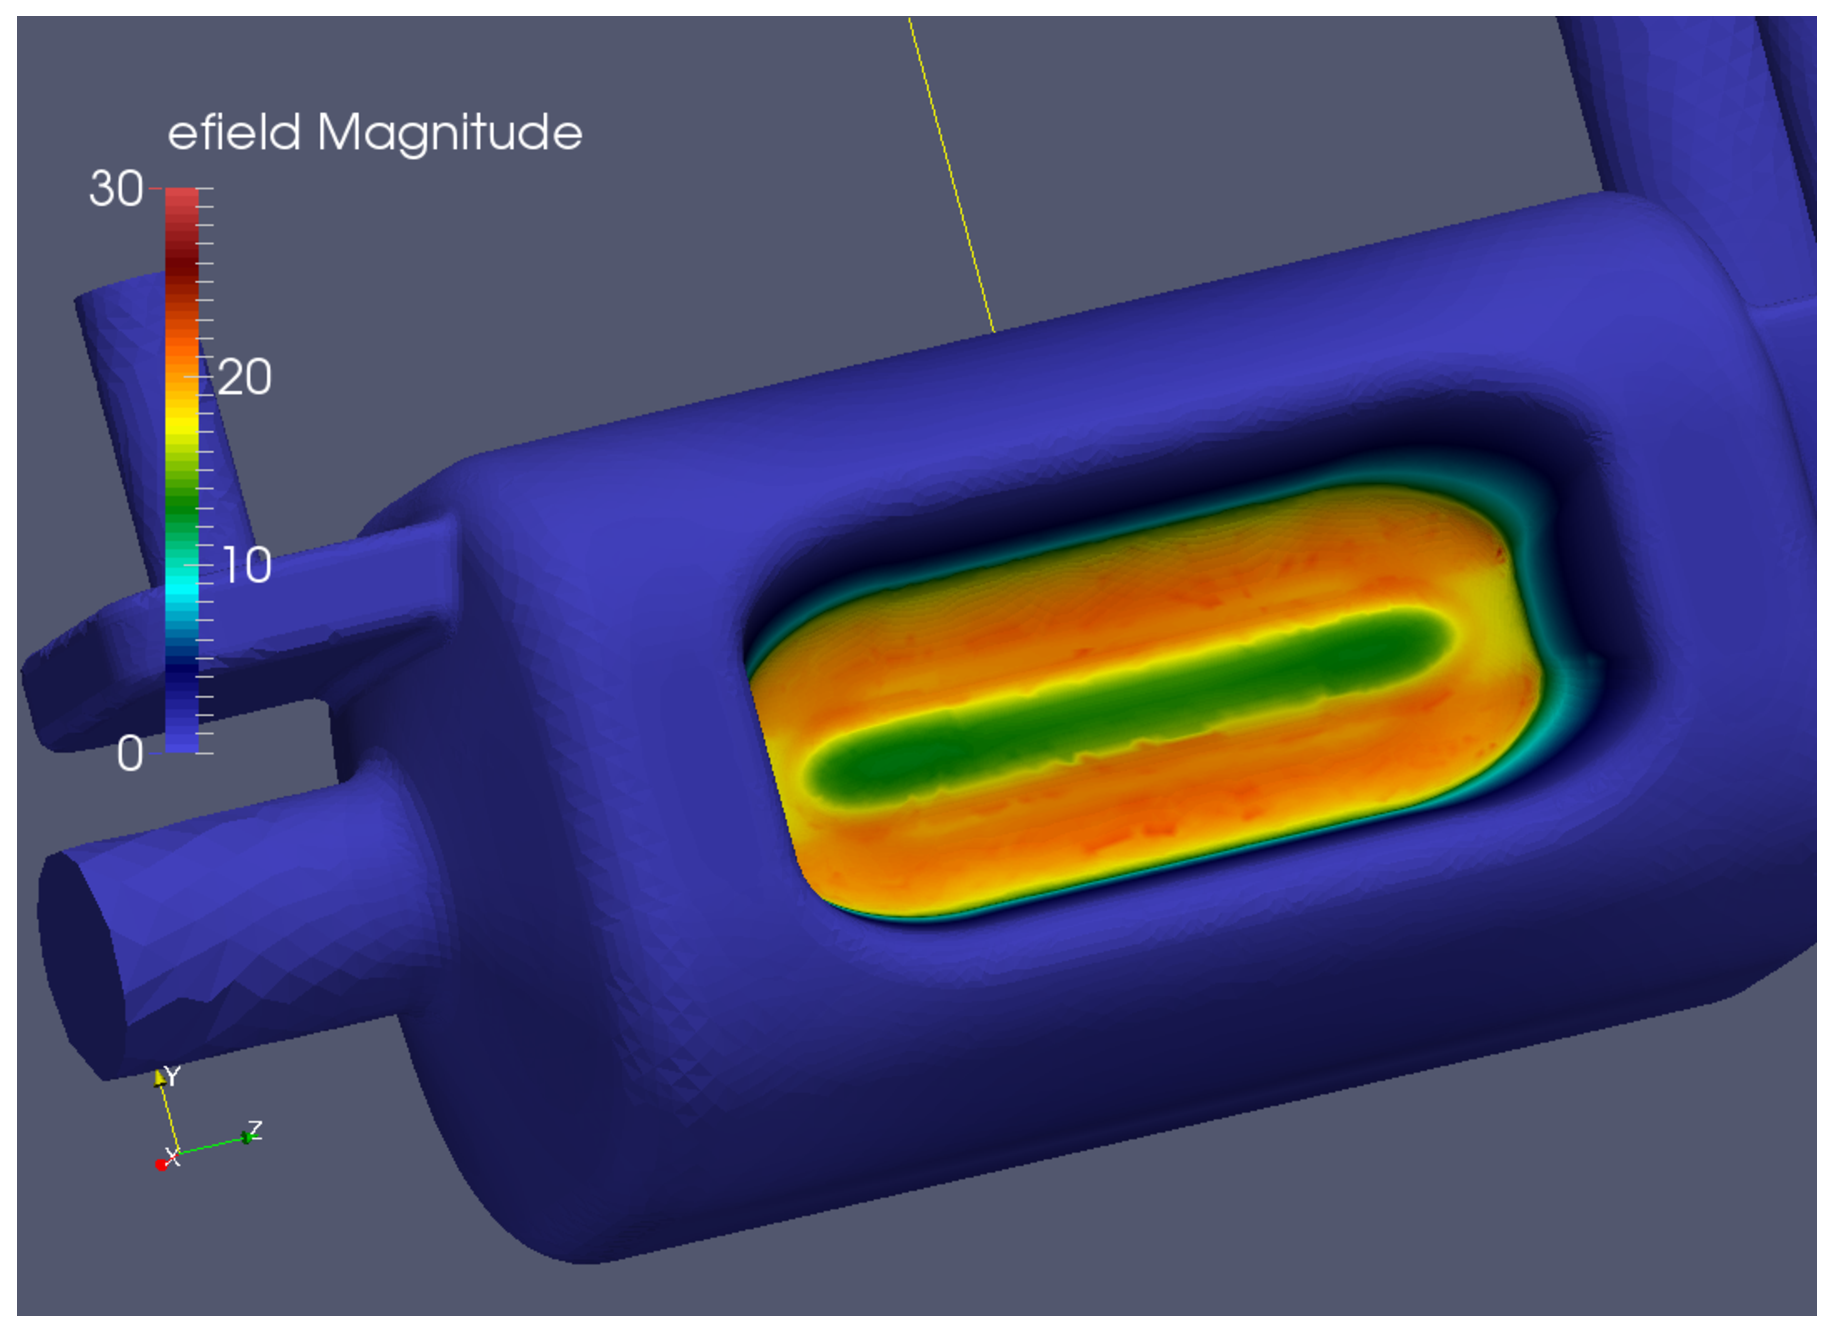
\includegraphics[width=0.43\textwidth]{../imp/figures/omega3p/cav17_al_3_ar_0p0125_386896_elems_e_field.eps}
  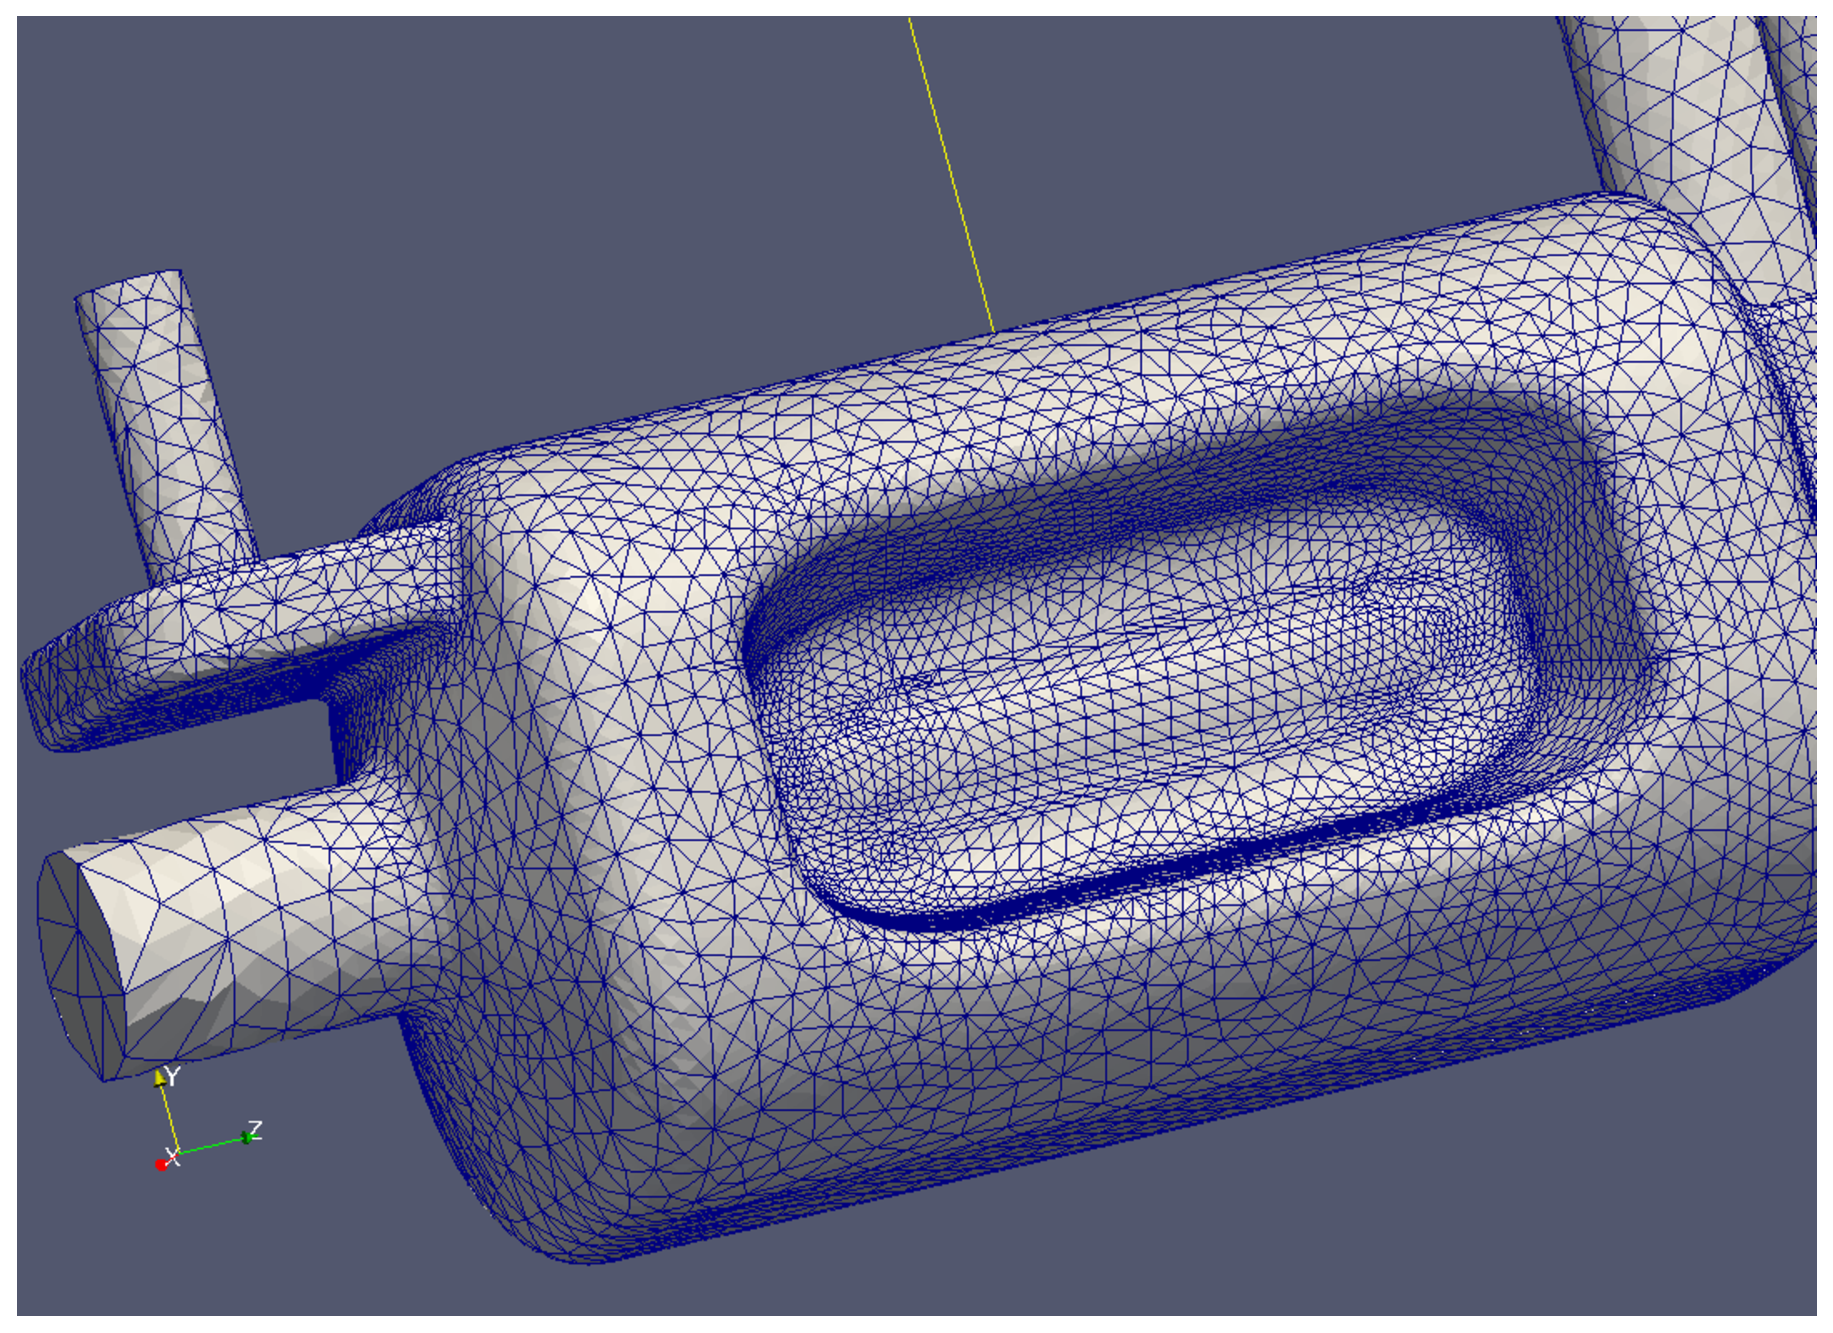
\includegraphics[width=0.43\textwidth]{../imp/figures/omega3p/cav17_al_3_ar_0p0125_386896_elems_mesh.eps}\\
  \small
    The first eigen-mode electric field (left column) and adapted meshes
    (right column) for the \texttt{pillbox} (top row) and \texttt{cav17}
    (bottom row) test cases.
\end{frame}


%----------- slide --------------------------------------------------%
\begin{frame}
  \frametitle{Omega3P Memory Use}
  {\centering
  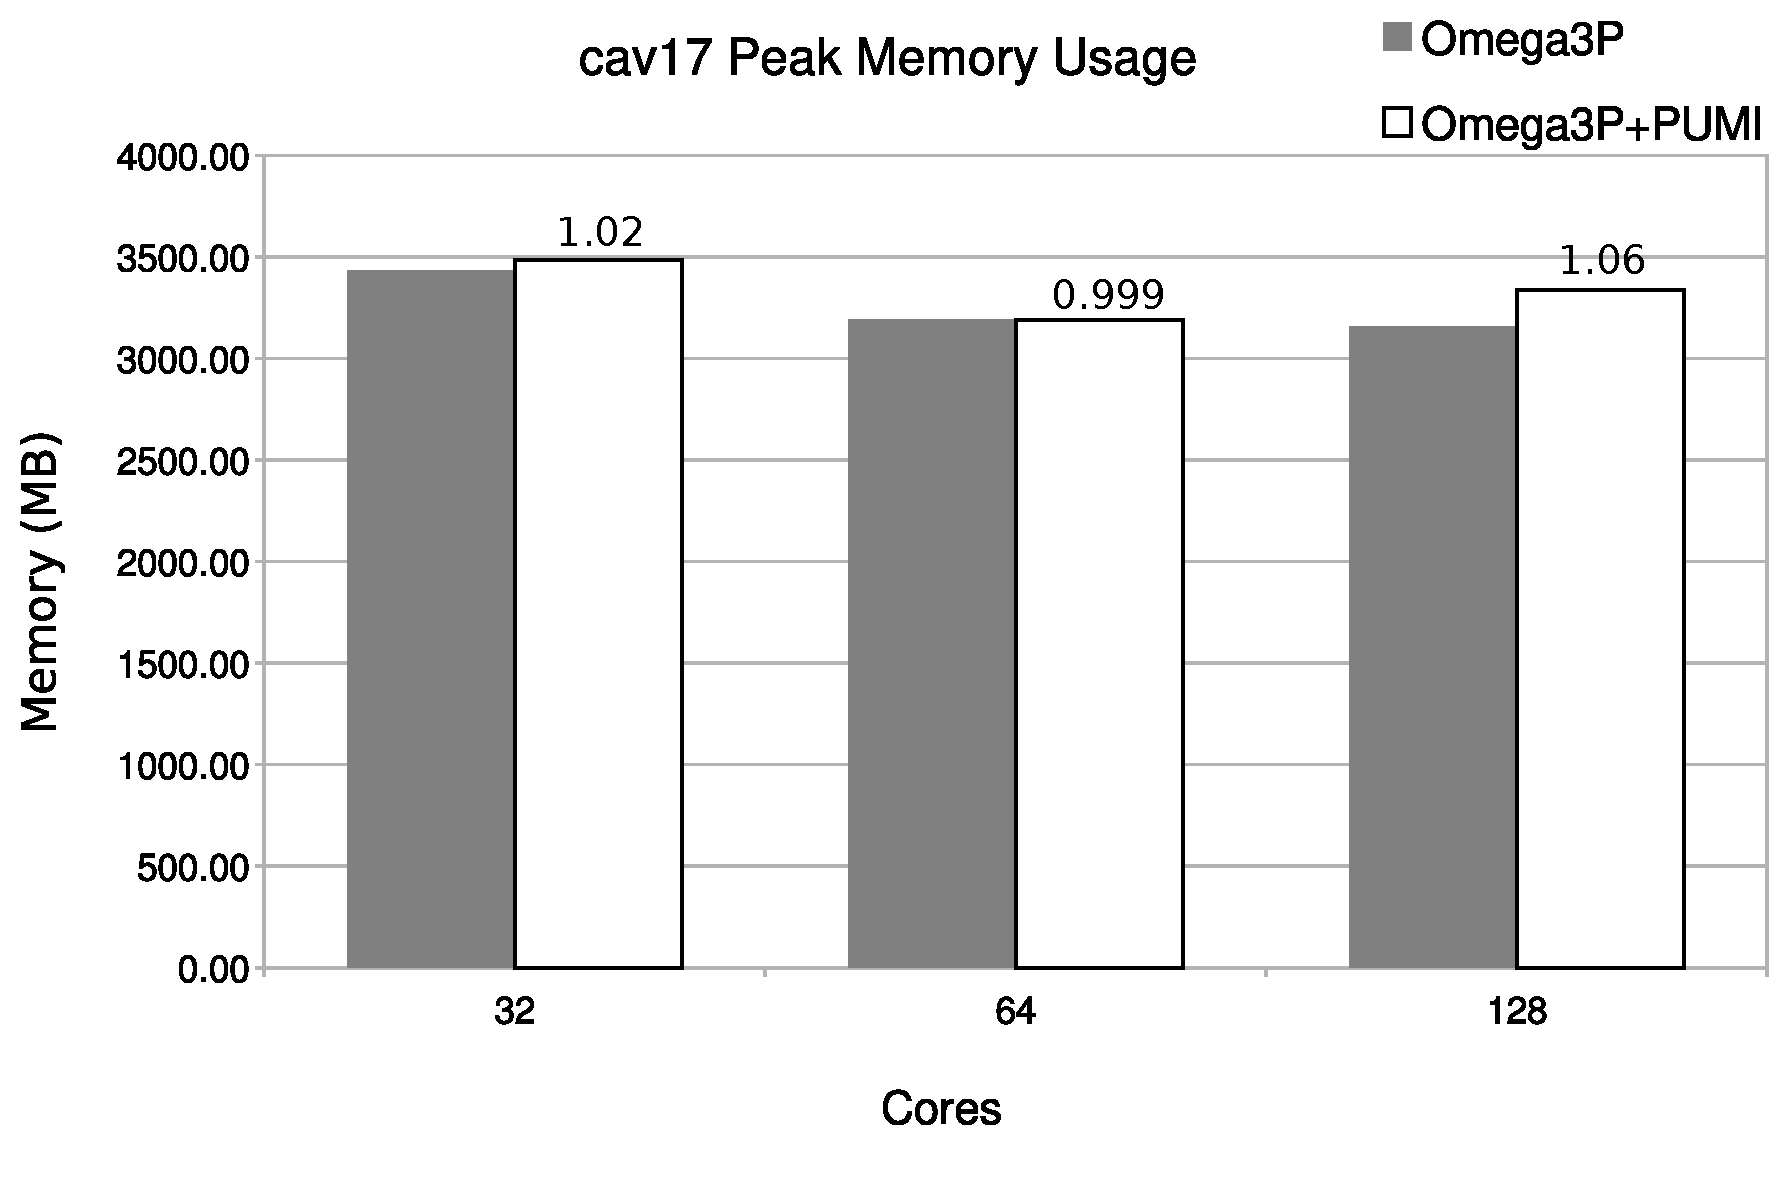
\includegraphics[width=.5\textwidth]{../imp/figures/omega3p/cav17-peak-mem.eps}
  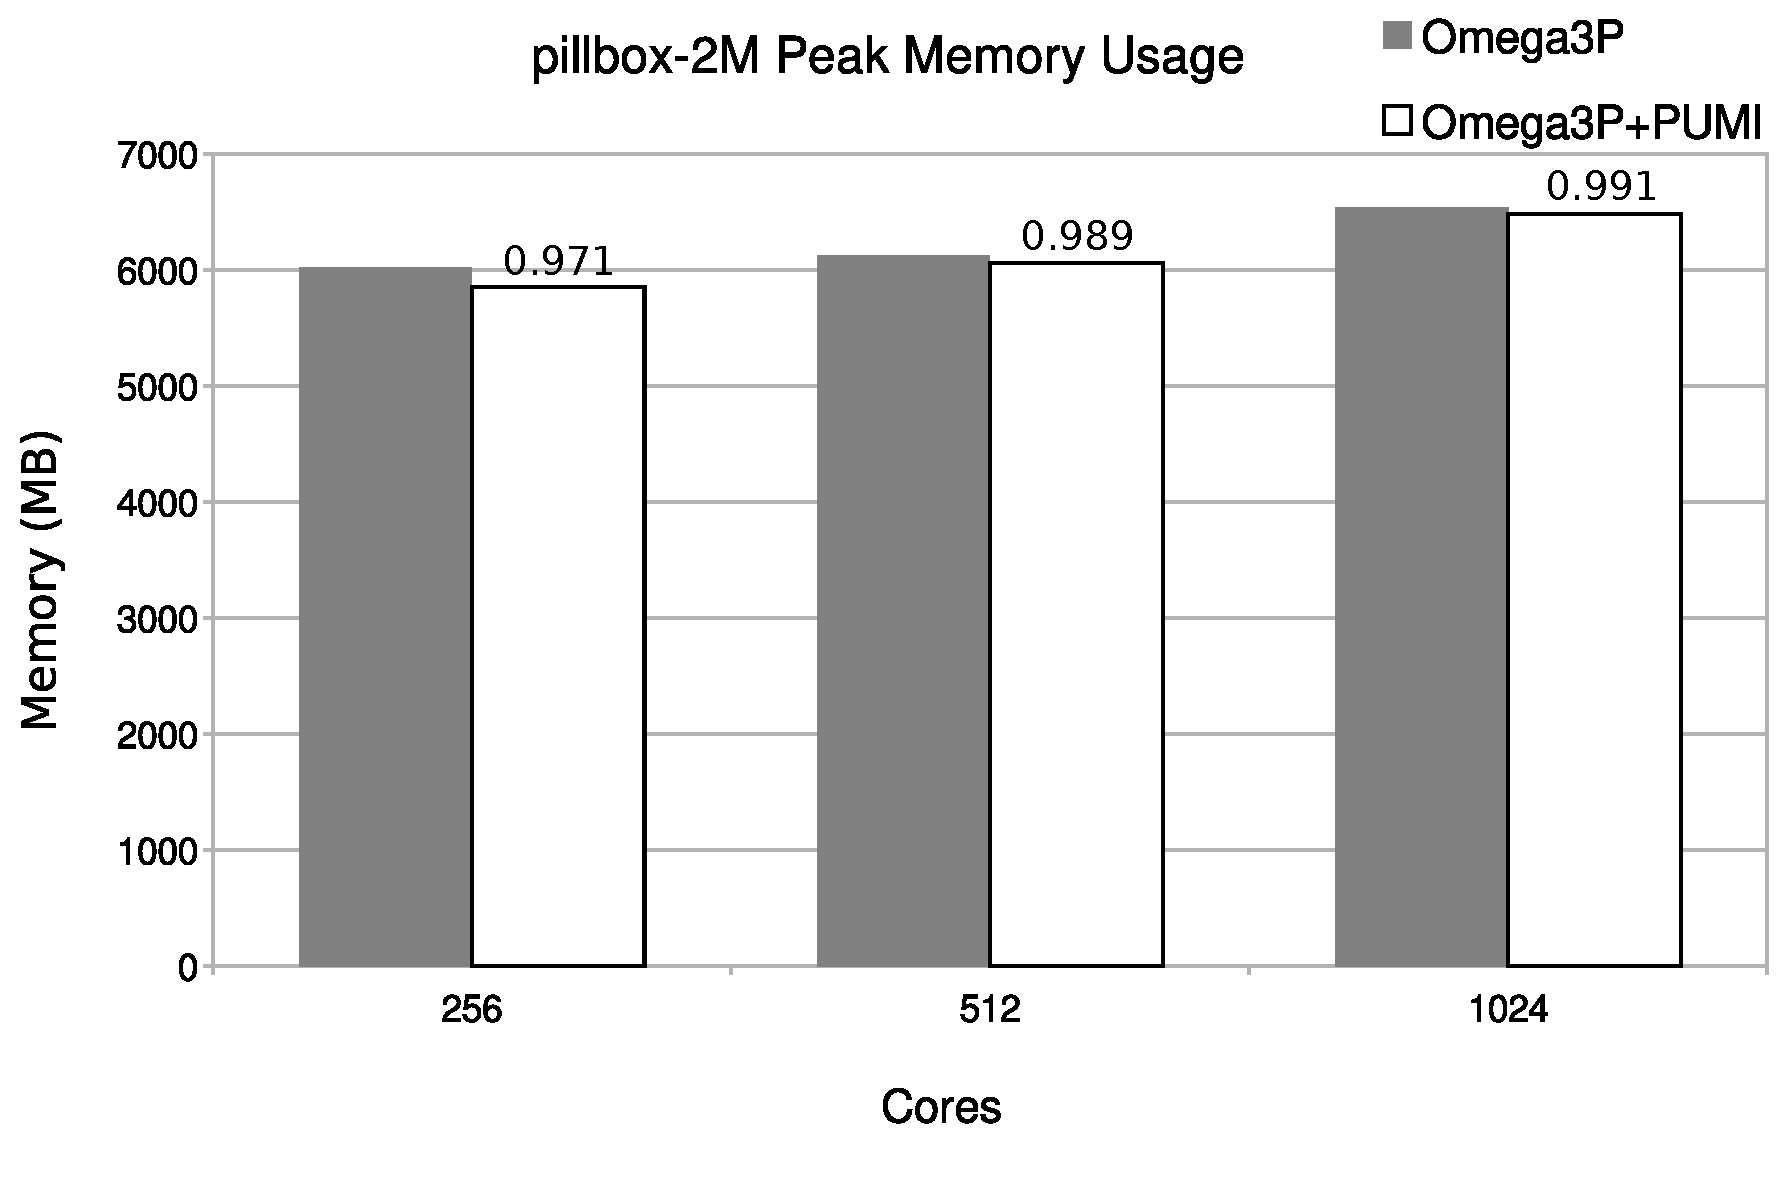
\includegraphics[width=.5\textwidth]{../imp/figures/omega3p/pillbox2M-peak-mem.eps}\\
  }
  Peak per-node memory usage for Omega3P and Omega3P+PUMI test cases
  (left){\texttt cav17} and (right) {\texttt pillbox-2M} 
  \begin{itemize}
    \item The increase in peak memory usage from storing two copies of the mesh and/or
      field data stored in memory is insignificant
  \end{itemize}
\end{frame}

%----------------------------------------------------------------------%
%----------- Section --------------------------------------------------%
%----------------------------------------------------------------------%
\section{Industrial Workflows}
\outline
\begin{frame}
  \frametitle{Constructing Industrial Workflows}
  Component based workflows, but often integrating with closed-source tools
  \begin{itemize}
    \item select best available tools that fit - not always bleeding edge
      (e.g., limited support for in-memory integration)
  \end{itemize}
  \medskip
  Workflow automation - reduce or eliminate the transfer of information 
  between user and software
\end{frame}

%----------- slide --------------------------------------------------%
\subsection{Micromechanical Device Analysis}
\begin{frame}
  \frametitle{Micromechanical Device Analysis}
  \begin{columns}
    \begin{column}{0.5\textwidth}
      Problem
      \begin{itemize}
        \item Multi-phase flow
        \item Viscous fluid ejected into air-filled chamber
        \item Actuated interface attached to fluid reservoir
      \end{itemize}
      Approach
      \begin{itemize}
        \item PHASTA interface tracking via level-sets
        \item Closed-source serial acutation code coupled to PHASTA via bulk
          APIs
        \item Anisotropic adaptation to refine at liquid-air interface
      \end{itemize}
      Result
      \begin{itemize}
        \item Simulations to drive design
      \end{itemize}
    \end{column}
    \begin{column}{0.5\textwidth}
      \includemedia[
        width=548pt,
        height=480pt,
        scale=0.2,
        activate=pageopen,
        addresource=animations/twoPhase_complete.mov,
        flashvars={%
          src=animations/twoPhase_complete.mov
          &autoPlay=true
          &loop=true
          &scaleMode=stretch
        }
      ]{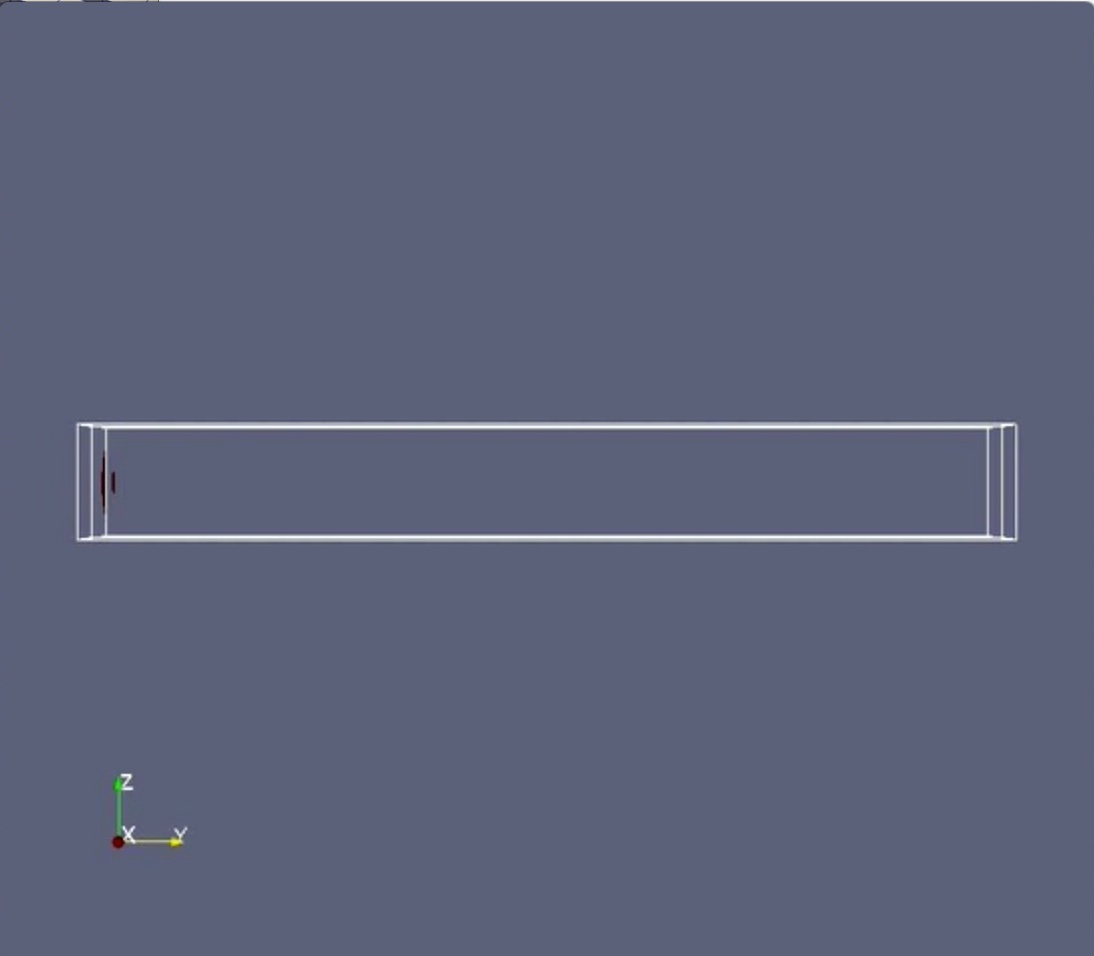
\includegraphics{animations/twoPhase_complete.jpeg}}{StrobeMediaPlayback.swf}

      \includemedia[
        width=884pt,
        height=720pt,
        scale=0.2,
        activate=pageopen,
        addresource=animations/AdaptiveTwoPhaseFlow.mov,
        flashvars={%
          src=animations/AdaptiveTwoPhaseFlow.mov
          &autoPlay=true
          &loop=true
          &scaleMode=stretch
        }
      ]{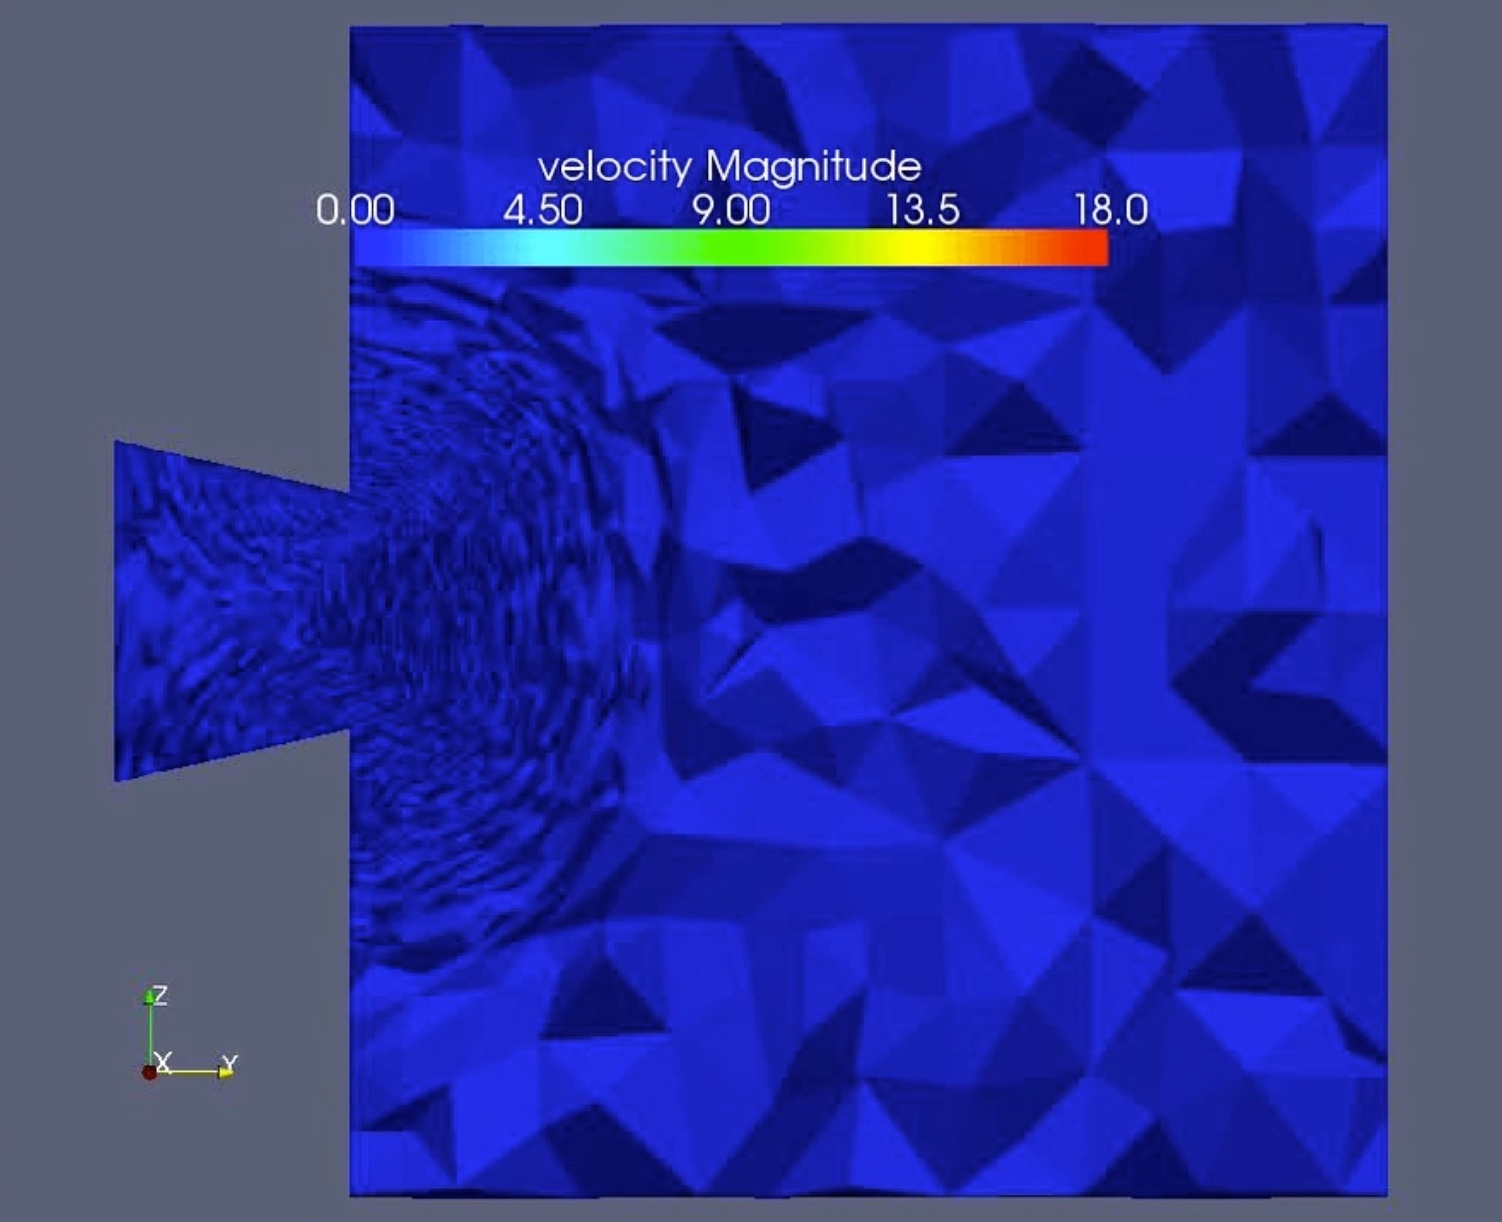
\includegraphics{animations/AdaptiveTwoPhaseFlow.jpeg}}{StrobeMediaPlayback.swf}
    \end{column}
  \end{columns}
\end{frame}

%----------- slide --------------------------------------------------%
\subsection{Semi-automated Pump Design}
\begin{frame}
  \frametitle{Semi-automated Pump Design}
  \begin{columns}
    \begin{column}{0.7\textwidth}
      Problem
      \begin{itemize}
        \item Study pump design over a range of operating conditions and
          geometric variations
        \item Reduce the time to run simulations - significant time spent in set up
      \end{itemize}
      Approach
      \begin{itemize}
        \item Simmetrix Abstract Model - define problem on topological
          definition of geometric model
        \item Simmetrix SimModeler - custom interface to define and export 
          attributes for ANSYS CFX
        \item ANSYS Workbench - couple with SLURM for automated job submission
      \end{itemize}
      Results
      \begin{itemize}
        \item Reduced time for set up - more time to focus on analysis results
        \item Helped design award winning pump
      \end{itemize}
    \end{column}
    \begin{column}{0.3\textwidth}
       \centering
       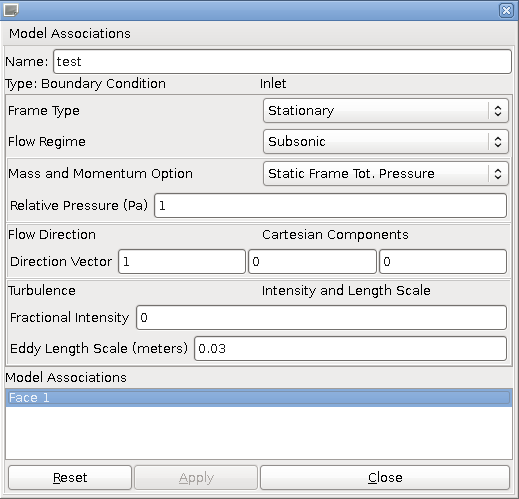
\includegraphics[width=\textwidth]{../applications/figures/simModelerInletBC.png}\\
       Custom attribute definition interface for the inlet boundary condition.
    \end{column}
  \end{columns}

\end{frame}

%----------- slide --------------------------------------------------%
\begin{frame}
  \frametitle{Semi-automated Pump Design}
  \centering
  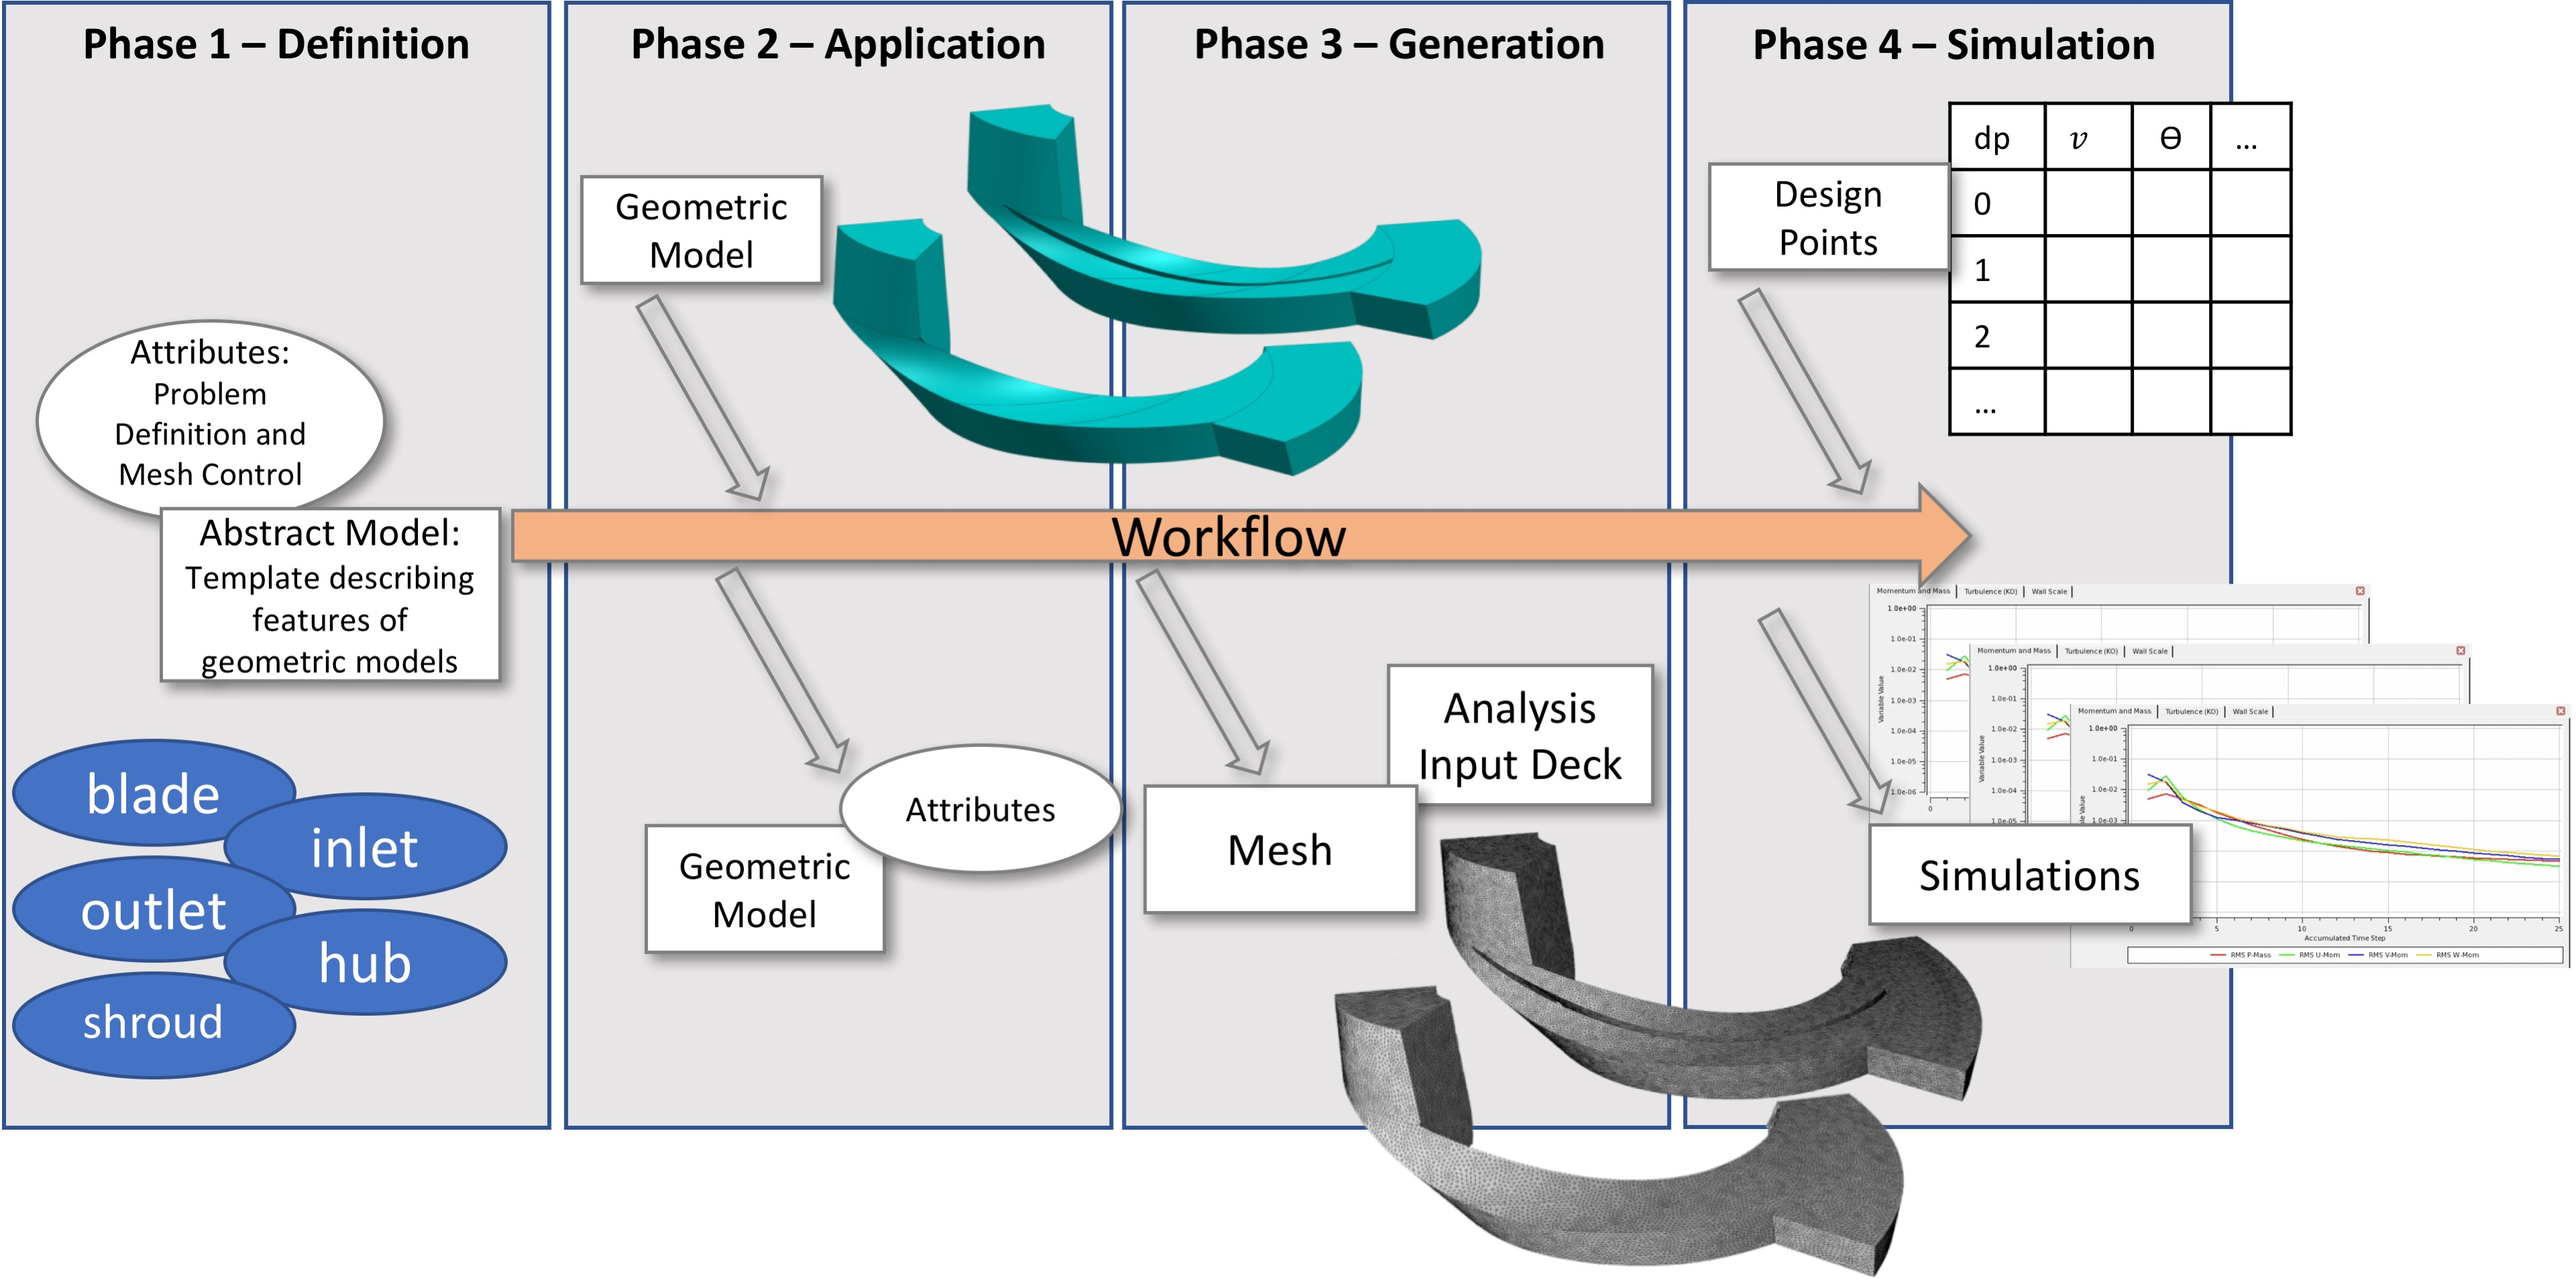
\includegraphics[width=\textwidth]{../applications/figures/pumpAbstractModelWorkflowSummary.jpg}\\
  Workflow from abstraction to simulation~\cite{simmodsuite}.
\end{frame}

%----------- slide --------------------------------------------------%
\subsection{High-fidelity Viscous Flow Simulation}
\begin{frame}
  \frametitle{Viscous Flows Simulations with the PHASTA Gateway}
  \begin{columns}
    \begin{column}{0.5\textwidth}
      Problem
      \begin{itemize}
        \item Support remote execution of workflows using
          best-practices for data management and reproducibility
      \end{itemize}
      Approach
      \begin{itemize}
        \item Airavata (PGA) - web-based interface for workflow execution and
          data management
      \end{itemize}
      Result
      \begin{itemize}
        \item Implemented interfaces for in-memory PHASTA-chef and PHASTA
          w/non-Newtonian material and partial-slip
        \item Support two TACC clusters and the CCI Blue Gene/Q
      \end{itemize}
    \end{column}
    \begin{column}{0.5\textwidth}
      \centering
      \includegraphics[width=0.7\textwidth]{../applications/figures/tseThinGap.jpg}\\
      \small
      Schematic of a screw extruder unstructured mesh with thin gaps.\\
      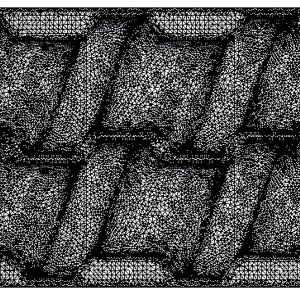
\includegraphics[height=2.0cm,keepaspectratio]{../applications/figures/tseMeshTwoThreads.png}
      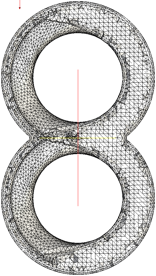
\includegraphics[height=2.0cm,keepaspectratio]{../applications/figures/tseMeshCrossSection.png}\\
      \includegraphics[height=2.0cm,keepaspectratio]{../applications/figures/tseFlowTwoThreads.png}
      \includegraphics[height=2.0cm,keepaspectratio]{../applications/figures/tseFlowCrossSection.png}\\
      \small
      Twin-screw extruder mesh (top) and axial velocity (bottom): (left) two
      threads of the screw and (right) cross-section of the extruder.
    \end{column}
  \end{columns}
\end{frame}

%----------------------------------------------------------------------%
%----------- Section --------------------------------------------------%
%----------------------------------------------------------------------%
\section{Conclusions and Future Work}
\outline

%----------- slide --------------------------------------------------%
\begin{frame}
  \frametitle{Conclusions}
  In parallel adaptive workflows bottlenecks exist during the 
  execution of the workflow, during the data transformation within workflow
  components, and during the data transfer between components.
  \medskip
  \begin{itemize}
    \item Applied workflow automation tools for ensembles of simulations and
      remote execution
    \item Our fast dynamic load balancing approach improves the linear algebra work
      performance of a computational fluid dynamics by 28\% over a graph-based
      partition, and improves scaling from 0.82 to 1.14, on 512Ki processes.
    \item We demonstrated bulk and atomic approaches for in-memory integration of
      existing components with over two orders of magnitude higher performance
      than file-based transfers.
  \end{itemize}
\end{frame}

%----------- slide --------------------------------------------------%
\begin{frame}
  \frametitle{Future Work}
  Load balancing
  \begin{itemize}
    \item NSF SI2 project to extend ParMA methods to applications with different
      mesh distributions or general information dependencies that can be
      expressed as an augmented graph.
  \end{itemize}
  In-memory coupling 
  \begin{itemize}
    \item Evaluating burst-buffers and pre-allocated stream buffers for writes
    \item Studying performance when streams written to DRAM instead of MCDRAM - cache eviction
  \end{itemize}
  Unstructured mesh workflows
  \begin{itemize}
    \item Integrating EngPar with NASA's FUN3D and PUMI with LLNL's MFEM.
    \item Developing workflows with industrial partners for heat-pump and 
      and underground reservoir applications that have evolving geometry.
    \item Expanding Science Gateway support and userbase.
  \end{itemize}
\end{frame}

%----------- slide --------------------------------------------------%
\begin{frame}
  \begin{center}
    {\huge
      Thank You\\
      \bigskip
      \bigskip
      \bigskip
      \bigskip
      \bigskip
      \large
      Questions?
    }
  \end{center}
\end{frame}

\bibliographystyle{scorec-refs/IEEEtran_rpi}
\begin{frame}
  \frametitle{References}
  \tiny
  \bibliography{scorec-refs/scorec-refs}
\end{frame}

%----------- slide --------------------------------------------------%
\begin{frame}
  \frametitle{Additional Slides}
\end{frame}

%----------- slide --------------------------------------------------%
\begin{frame} \frametitle{Parallel Adaptive Simulation Workflows} 
  Interaction of multiple components required to form adaptive workflows.\\
  \includegraphics[width=.95\textwidth]{../workflows/figures/workflowComponentInteractions.jpg}
\end{frame}

%----------- slides --------------------------------------------------%
\begin{frame}
  \frametitle{Key Unstructured Mesh Workflow Components}
  \begin{columns}
    \begin{column}{0.6\textwidth}
      Geometric Model Definition \& Interrogation
      \begin{itemize}
        \item topology and shape
        \item support multiple sources
      \end{itemize}
      Mesh Generation
      \begin{itemize}
        \item automatic and robust
        \item interface to kernels
      \end{itemize}
      Mesh Data Structure 
      \begin{itemize}
        \item O(1) access to adjacencies
        \item association with geometric model
      \end{itemize}
      Mesh Adaptation
      \begin{itemize}
        \item size-field driven refinement \& coarsening
        \item support local-solution transfer
      \end{itemize}
    \end{column}
    \begin{column}{0.4\textwidth}
      \centering
      \tiny
      \includegraphics[width=.8\textwidth]{../imp/figures/upright/upright-initial.png}\\
      RPI Formula Hybrid suspension upright
      \includegraphics[width=.9\textwidth]{../workflows/figures/digimouse_edmans.png}\\
      Segmented Digimouse~\cite{edmansMeshMonteCarlo2015}
      \includegraphics[width=.8\textwidth]{../workflows/figures/landersMesh.pdf}\\
      Landers fault-system~\cite{seisSolGeomPoster,seisSolGordonBell2014}
    \end{column}
  \end{columns}
\end{frame}

%----------- slide --------------------------------------------------%
\begin{frame}
  \frametitle{Stream Pre-allocation}
  \centering
  \includegraphics[width=0.8\textwidth]{../imp/results/streamPrealloc/streamPreallocWriteEffectiveBandwidth.eps}\\
  Streaming write performance with and without preallocation on a single node
    of ALCF Theta in the cache-quad configuration.
\end{frame}

%%----------- slide --------------------------------------------------%
\begin{frame}
  \frametitle{Component Graph Distance}
  \small 
  Components in one of four parts of the MPAS 60km ocean mesh.  Dark shaded
  elements are isolated and light shaded elements are on a different part.
  \begin{columns}
    \begin{column}{0.5\textwidth}
      \centering
      \tiny 
      \includegraphics[width=.9\textwidth]
        {../parmaimprovement/figs/compDist/p2core.eps}\\
      Component core vertices.\\
      \includegraphics[width=.9\textwidth]
        {../parmaimprovement/figs/compDist/p2distComps_nocolor.eps}\\
      Offset vertex graph distance.
    \end{column}
    \centering
    \begin{column}{0.4\textwidth}
      \tiny 
      \begin{column}{0.5\textwidth}
        \includegraphics[width=\textwidth]
          {../parmaimprovement/figs/compDist/p2distComps_nocolor_dccompsA.eps} \\
        \includegraphics[width=\textwidth]
          {../parmaimprovement/figs/compDist/p2distComps_nocolor_dccompsB.eps} \\
        \includegraphics[width=\textwidth]
          {../parmaimprovement/figs/compDist/p2distComps_nocolor_dccompsC.eps}
      \end{column}
      \begin{column}{0.5\textwidth}
        \includegraphics[width=\textwidth]
          {../parmaimprovement/figs/compDist/p2distCompsOff_nocolor_dccompsA.eps} \\
        \includegraphics[width=\textwidth]
          {../parmaimprovement/figs/compDist/p2distCompsOff_nocolor_dccompsB.eps} \\
        \includegraphics[width=\textwidth]
          {../parmaimprovement/figs/compDist/p2distCompsOff_nocolor_dccompsC.eps}
      \end{column}
      \\Graph distance of disconnected components A, B, and C, before 
      (left) and after (right) the offset is applied.
    \end{column}
  \end{columns}
\end{frame}

%%----------- slide --------------------------------------------------%
\begin{frame}
  \frametitle{Entity Level Selection Metric}
  \begin{itemize}
    \item Iterate over the boundary vertices in descending order of distance
    \item Construct the cavity of bounded elements that have not been tagged 
      for migration
    \item Find the neighbor that shares the most cavity mesh entities 
      - highest surface area
    \item Select the cavity for migration if:
      \begin{itemize}
        \item The cavity contains a small number of elements \emph{and}
        \item The weight transfer limit to the neighboring part has not been met
      \end{itemize}
    \item Multiple passes are ran with increasing cavity size limits 
      - choose the smallest cavities first to decrease part surface area
  \end{itemize}
  \begin{columns} 
    \begin{column}{0.4\textwidth}
      \centering
      \includegraphics[width=\textwidth]{figs/vtxCavitiesFaceDisconnected.eps}\\
    \end{column}
    \begin{column}{0.3\textwidth}
      \centering 
      \includegraphics[width=\textwidth]{{figs/vertexCavities.png}.eps}\\
    \end{column}
    \begin{column}{0.45\textwidth}
      \tiny
      \begin{tabular}{l|cccccc} 
        & \multicolumn{6}{|c}{Cavity}\\
        Ent. & a & b & c & d & e & f \\
        \hline
        Vtx  & 1 & 1 & 1 & 1 & 1 & 0 \\
        Edge & 7 & 7 & 8 & 3 & 3 & 0 \\
        Face & 4 & 6 & 6 & 2 & 2 & 0 \\
      \end{tabular}\\
      Reduction in number of mesh \\
      entities classified on $P^2_i$ for cavities.
    \end{column}
  \end{columns}
  \tiny
  Face disconnected (a-c) and connected (d-f) cavities.  The bounding vertex is
  marked with a disc, vertices classified on the partition model face $P^2_i$
  with a circle, and, in (f), an interior vertex with a square. 
\end{frame}

%%----------- slide --------------------------------------------------%
\begin{frame}
  \frametitle{Diffusion from Heavy to Light}
  \centering
  \includemedia[
    activate=pageopen,
    addresource=animations/ocean60km.mov,
    flashvars={%
       src=animations/ocean60km.mov
      &autoPlay=true
      &loop=true
      &scaleMode=stretch
    }
  ]{\includegraphics[width=\textwidth]{animations/ocean60km.png}}{StrobeMediaPlayback.swf}
  The heavy part on the left sends elements to the neighboring parts.
\end{frame}

%----------- slide --------------------------------------------------%
\begin{frame}
  \frametitle{In-Memory Approaches Cont.}
  Component Models
  \begin{itemize}
    \item Object Management Group CCM, Microsoft .Net and COM, etc. ...
    \item Standards for reusable components that support interoperability
    \item Support for runtime on HPC systems may be a problem
    \item May be a logical choice for components spanning multiple languages
      without any existing coupling mechanisms
    \item Helios (ARMY) rotorcraft framework uses a Python infrastructure
  \end{itemize}
  \centering
  \includegraphics[width=.5\textwidth]{../workflows/figures/helios.png}\\
  \tiny
  (\url{https://www.nas.nasa.gov/assets/pdf/ams/2016/AMS_20160223_Wissink.pdf})
\end{frame}

%----------- slide --------------------------------------------------%
\begin{frame}
  \frametitle{In-Memory Approaches Cont.}
  Google Flatbuffers and Cap'n Proto
  \begin{itemize}
    \item Protocols for serialized data transfers
    \item Users define and implement format for transfers
    \item Support for `zero copy' mode - read directly from transferred buffer
    \item Logical choice for bulk interactions between multiple components 
  \end{itemize}
  ADIOS (Oak Ridge National Laboratory)
  \begin{itemize}
    \item Single set of API for parallel file I/O and in-memory coupling
    \item In-memory coupling is via executables through file abstraction
    \item Logical choice for set of components needing parallel file I/O that
      can operate effectively in executable-based in-memory coupling model
  \end{itemize}
\end{frame}

%----------- slide --------------------------------------------------%
\begin{frame}
  \frametitle{Albany POSIX files versus APIs}
  \begin{columns}
    \begin{column}{0.5\textwidth}
      \begin{itemize}
        \item Factor of two performance advantage of in-memory transfers of
          fields and mesh data versus mesh writing to POSIX files.
        \item Stable in-memory transfer times; 
          6\% imbalance (max cycle time / avg cycle time) versus 
          22\% POSIX imbalance at 512 cores
      \end{itemize}
    \end{column}
    \begin{column}{0.5\textwidth}
      \includegraphics[width=\textwidth]{../imp/results/albany/compare.eps}\\
      \small
      Average per-cycle file writing and in-memory transfer times.  Minimum and
      maximum bars are only shown for the 512 core file writing data point where
      they are 6\% more, or less, than the mean, respectively.
    \end{column}
  \end{columns}
\end{frame}

%----------- slide --------------------------------------------------%
\begin{frame}
  \frametitle{Partitioning to 1,048,576 Parts}
  \small
  X+ParMA : X=\{Zoltan PHG, ParMETIS Part k-way, RIB\}
  \tiny
  \begin{tabular}{ l|ccccccc }
    density & elements    & parts    & target parts & $I^0$ & $I^1$ & $I^2$ & $I^3$  \\
    \hline
    small   & 1.6*10$^9$  & 2$^{17}$ & 2$^{20}$     & 1.06  & 1.06  & 1.06  & 1.07  \\
    medium  & 12.9*10$^9$ & 2$^{17}$ & 2$^{20}$     & 1.05  & 1.06  & 1.07  & 1.07  \\
    large   & 12.9*10$^9$ & 2$^{17}$ & 2$^{19}$     & 1.05  & 1.06  & 1.07  & 1.07  \\
  \end{tabular}
  \npstyleenglish
  \nprounddigits{2}
  \begin{tabular}{ c c c c N{4}{2} N{4}{2} N{1}{2} N{1}{2} N{1}{2} N{1}{2} N{3}{2} }
    \tiny
           &         &        &            &                    & {decrease}          &                             &                             &                             &                             & \\
    scope  & density & method & stage      & {avg vtx}          & {avg vtx (\%)}      & \multicolumn{1}{c}{$I^{0}$} & \multicolumn{1}{c}{$I^{1}$} & \multicolumn{1}{c}{$I^{2}$} & \multicolumn{1}{c}{$I^{3}$} & {tot (s)}\\
    \hline
    local  & small   & rib    & afterSplit & 455.084            &                     & 1.34                        & 1.18                        & 1.1299999999999999          & 1.1299999999999999          & 10.666808\\
           &         &        & afterParma & 427.63400000000001 & 6.4190405814317897  & 1.07                        & 1.06                        & 1.05                        & 1.05                        & 8.9435760000000002\\
           &         & pmetis & afterSplit & 427.04899999999998 &                     & 1.63                        & 1.32                        & 1.1299999999999999          & 1.1200000000000001          & 8.9928939999999997\\
           &         &        & afterParma & 418.80900000000003 & 1.9674839843460745  & 1.05                        & 1.05                        & 1.04                        & 1.04                        & 9.4759810000000009\\
           & medium  & rib    & afterSplit & 2825.4839999999999 &                     & 1.31                        & 1.1399999999999999          & 1.08                        & 1.07                        & 54.315722999999998\\
           &         &        & afterParma & 2751.97            & 2.6713227251750515  & 1.06                        & 1.05                        & 1.04                        & 1.05                        & 48.810063999999997\\
           &         & pmetis & afterSplit & 2687.7469999999998 &                     & 1.35                        & 1.1399999999999999          & 1.1100000000000001          & 1.1100000000000001          & 59.813361999999998\\
           &         &        & afterParma & 2671.3220000000001 & 0.61486410099567124 & 1.05                        & 1.05                        & 1.04                        & 1.05                        & 36.149090000000001\\
           & large   & rib    & afterSplit & 5273.8810000000003 &                     & 1.1599999999999999          & 1.1299999999999999          & 1.1200000000000001          & 1.1299999999999999          & 42.686045999999997\\
           &         &        & afterParma & 5122.8519999999999 & 2.9481429484982336  & 1.05                        & 1.04                        & 1.04                        & 1.05                        & 52.866339000000004\\
           &         & pmetis & afterSplit & 5132.3829999999998 &                     & 1.21                        & 1.0900000000000001          & 1.1000000000000001          & 1.1000000000000001          & 37.019446000000002\\
           &         &        & afterParma & 5102.2049999999999 & 0.59146976650290561 & 1.04                        & 1.04                        & 1.04                        & 1.04                        & 41.554078000000004\\
    global & small   & rib    & afterSplit & 470.10199999999998 &                     & {\textbf{3.09}}             & 2.0699999999999998          & 1.45                        & 1                           & 103.136197\\
           &         &        & afterParma & 445.43400000000003 & 5.5379697104396941  & {\textbf{1.06}}             & 1.04                        & 1.03                        & 1.04                        & 20.226883000000001\\
           & large   & rib    & afterSplit & 5367.2979999999998 &                     & 2.4900000000000002          & 1.7                         & 1.29                        & 1                           & 96.792032000000006\\
           &         &        & afterParma & 5228.808           & 2.6485960088800331  & 1.05                        & 1.02                        & 1.03                        & 1.04                        & 379.83779700000002\\
  \end{tabular}
\end{frame}

%----------- slide --------------------------------------------------%
\begin{frame}
  \frametitle{High-fidelity Viscous Flow Simulation}
  \begin{columns}
    \begin{column}{0.5\textwidth}
      Problem
      \begin{itemize}
        \item flow of viscous fluid through twin-screw extruder (TSE)
      \end{itemize}
      Approach
      \begin{itemize}
        \item PHASTA non-Newtonian materials w/ partial slip boundary conditions
        \item Simmetrix MeshSim Advanced mesh generation
      \end{itemize}
      Result
      \begin{itemize}
        \item Demonstrated parallel analysis capability
      \end{itemize}
    \end{column}
    \begin{column}{0.5\textwidth}
      \centering
      \includegraphics[width=0.7\textwidth]{../applications/figures/tseThinGap.jpg}\\
      \small
      Schematic of a screw extruder unstructured mesh with thin gaps.\\
      \includegraphics[height=2.0cm,keepaspectratio]{../applications/figures/tseMeshTwoThreads.png}
      \includegraphics[height=2.0cm,keepaspectratio]{../applications/figures/tseMeshCrossSection.png}\\
      \includegraphics[height=2.0cm,keepaspectratio]{../applications/figures/tseFlowTwoThreads.png}
      \includegraphics[height=2.0cm,keepaspectratio]{../applications/figures/tseFlowCrossSection.png}\\
      \small
      TSE mesh (top) and axial velocity (bottom): (left) two threads of the
      screw and (right) cross-section of the extruder.
    \end{column}
  \end{columns}
\end{frame}


%----------- slide --------------------------------------------------%
\begin{frame}
  \frametitle{Related Publications}
  Unstructured Mesh Tools\\
  {\footnotesize
  \begin{itemize}
    \item \bibentry{rasquinCise2014}
    \item \bibentry{ibanez2016pumi}
  \end{itemize}
  }
  Workflows\\
  {\footnotesize
  \begin{itemize}
    \item \bibentry{smithXsede15}
    \item \bibentry{smith2016building}
    \item \bibentry{shephard2013bringing}
  \end{itemize}
  }
\end{frame}

\end{document}
